%%%%%%%%%%%%%%%%%%%%%%%%%%%%%%%%%%%%%%%%%%%%%%%%%%%%%%%%%%%%%%%%%%%%%%%%
%                                                                      %
% LaTeX, FIIW thesis template                                          %
% 19/12/2023 v1.3                                                      %
%  TODOs:                                                              %
%   - Translate all comments to English                                %
%%%%%%%%%%%%%%%%%%%%%%%%%%%%%%%%%%%%%%%%%%%%%%%%%%%%%%%%%%%%%%%%%%%%%%%%


% \documentclass[11pt,a4paper,twoside,openright]{report}
\documentclass[11pt,a4paper]{report}
% Indien je je thesis recto-verso wil afdrukken gebruik je onderstaande opties i.p.v. bovenstaande
%\documentclass[11pt,a4paper,twoside,openright]{report}
\usepackage[a4paper,left=3.5cm, right=2.5cm, top=3.5cm, bottom=3.5cm]{geometry}
\usepackage{graphicx}
\graphicspath{{./figs/}}                        % set graphics path to figs folder, ie now all file imports can be referenced relative to figs
\usepackage[latin1]{inputenc}                   % om niet ascii karakters rechtstreeks te kunnen inputten
%\usepackage[utf8]{inputenc}                    % commentarieer deze regel uit als je utf8 encoded files gebruikt in plaats van latin1
\usepackage[backend=biber, style=ieee, 
citestyle=numeric-comp, maxnames=99]{biblatex}  % make use of the biblatex package to cite references
\addbibresource{bib.bib}
\AtBeginBibliography{\footnotesize}

\usepackage{cmbright}                           % new improved font
\usepackage{listings}             		        % voor het weergeven van broncode
\usepackage{minted}                     % for beautiful listings
\usemintedstyle{borland}
\usepackage{verbatim}					        % weergeven van code, commando's, ...
\usepackage{hyperref}					        % maak PDF van de thesis navigeerbaar
\usepackage{url}						        % URL's invoegen in tekst met behulp van \url{http://}
\usepackage[small,bf,hang]{caption}             % om de captions wat te verbeteren
\usepackage[final]{pdfpages}                    % gebruikt voor het invoegen van het artikel in pdf-formaat
%\usepackage{pslatex}					        % andere lettertype's dan de standaard types

%\usepackage{sectsty}					        % aanpassen van de fonts van sections en chapters
%\allsectionsfont{\sffamily}
%\chapterfont{\raggedleft\sffamily}

\usepackage{float}                              % De optie H voor de plaatsing van figuren op de plaats waar je ze invoegt. bvb. \begin{figure}[H]
%\usepackage{longtable}					        % tabellen die over meerdere pagina's gespreid worden
%\usepackage[times]{quotchap}                   % indien je fancy hoofdstuktitels wil
%\usepackage[none]{hyphenat}
%\usepackage{latexsym}
\usepackage{amsmath}
\usepackage{amssymb}
\usepackage{siunitx}
\sisetup{detect-all}
\usepackage[acronym,xindy]{glossaries}
\makenoidxglossaries
\usepackage[version=4]{mhchem}                  % chemical formulas
\usepackage{tabularx}
\usepackage{booktabs}                           % nice tables
\usepackage{array}                              % fixed-width columns in tables

%%%% Tikz %%%%
\usepackage{pgfplots}
\DeclareUnicodeCharacter{2212}{−}
\usepgfplotslibrary{groupplots,dateplot}
\usetikzlibrary{patterns,shapes.arrows}
\pgfplotsset{compat=newest}
%%%%%%%%%%%% MAKE FIGURES MORE UNIFORM %%%%%%%%%%%%
\definecolor{darkgray176}{RGB}{176,176,176}
\definecolor{color0}{RGB}{255,127,14}
\definecolor{color1}{RGB}{44,160,44}
\pgfplotsset{
    every axis/.append  style={
        title style={draw=none},
        label style={font=\small},
        legend style={
            fill opacity=0.8,
            nodes={scale=0.8, transform shape}, {draw=none}
        },
        tick align=outside,
        tick pos=left,
        x grid style={darkgray176},
        xtick style={color=black},
        y grid style={darkgray176},
        ytick style={color=black},
        grid=both,
    },
    every axis plot/.append style={
        line width=1.0pt,
        mark size=1,
    },
}

\usepackage{caption}
\usepackage{subcaption}


%%%%%%%%%%%% choose your campus and language %%%%%%%%%%%%
\usepackage{fiiw} 



%door onderstaande regels in commentaar te zetten, of op false, kan je pagina's weglaten
%bijvoorbeeld het weglaten van een voorwoord, lijst met symbolen, ...
%%%%%%%%%%%%%%%%%%%%%%%%%%%%%%%%%%%%%%%%%%%%%%%%%%%%%%%%%%%%%%%%%%%%%%%%%%%%%%%%%%%%%%%%
%voorwoord toevoegen?
\acknowledgementspagetrue
\acknowledgements{preface}			%.tex file met daarin het voorwoord
%abstract toevoegen?
\abstractpagetrue
\abstracts{abstract}					%.tex file met daarin het abstract
%lijst van figuren toevoegen?
%\listoffigurespagetrue
%lijst van tabellen toevoegen?
%\listoftablespagetrue
%lijst van symbolen toevoegen?
%\listofsymbolspagetrue
%\listofsymbols{symbolen}				%.tex file met daarin de lijst van symbolen


% Information about your discipline
%%%%%%%%%%%%%%%%%%%%%%%%%%%%%%%%%%%%%%%%%%%%%%%

\opleiding{discipline name}
\afdeling{specialisation}
\campus{gent}                       % Define your campus and language (append "eng" to load the English template)
                                            % campuses: denayer, geel, gent, groept, brugge (denayereng, geeleng, ghenteng, groupteng, brugeseng)
\title{Title Masterproef}
\subtitle{Subtitle (optional)}
\forenameA{first name}
\surnameA{last name}
\forenameB{} %keep empty if no 2nd author
\surnameB{} %keep empty if no 2nd author
\academicyear{2024 - 2025}


\promotorA[Promotor(en)]{My Promotor} %for English use Supervisor(s)
\promotorB[Co-promotor(en)]{My Co-promotor\\My company promotor}

\loadLanguage% keep this untouched

% generated by Gilles Callebaut with the script: https://github.com/DRAMCO/writing-scientific-papers-in-latex-tips-and-tricks/blob/main/glossaries/merge_abbr.py

% generated by Gilles Callebaut with the Github action: https://github.com/GillesC/action-abbreviations-latex

%%%%%%%%%%%% 2 %%%%%%%%%%%%
\newacronym{2d}{2D}{two-dimensional}
%%%%%%%%%%%% 3 %%%%%%%%%%%%
\newacronym{3d}{3D}{three-dimensional}
\newacronym{3gpp}{3GPP}{3rd generation partnership project}
%%%%%%%%%%%% 4 %%%%%%%%%%%%
\newacronym{4g}{4G}{fourth-generation}
%%%%%%%%%%%% 5 %%%%%%%%%%%%
\newacronym{5g}{5G}{fifth-generation}
%%%%%%%%%%%% 6 %%%%%%%%%%%%
\newacronym{6dof}{6DoF}{six degrees of freedom}
\newacronym{6g}{6G}{sixth-generation}
%%%%%%%%%%%% A %%%%%%%%%%%%
\newacronym{abp}{ABP}{authentication by personalisation}
\newacronym{ac}{AC}{alternating current}
\newacronym{aclr}{ACLR}{adjacent channel leakage ratio}
\newacronym{adc}{ADC}{analog-to-digital converter}
\newacronym{adr}{ADR}{adaptive data rate}
\newacronym{aes}{AES}{Advanced Encryption Standard}
\newacronym{afe}{AFE}{analog front end}
\newacronym{ag}{AG}{array gain}
\newacronym{agc}{AGC}{automatic gain controller}
\newacronym{agps}{A-GPS}{Assisted Global Positioning System} %bestaat al :) % Aha, dan maak ik er wel Assisted gps van!
\newacronym{ai}{AI}{artificial intelligence}
\newacronym{alk}{ALK}{Alkaline}
\newacronym{am}{AM}{amplitude modulation}
\newacronym{amam}{AM/AM}{amplitude modulation to amplitude modulation}
\newacronym{amc}{AMC}{automatic modulation classification}
\newacronym{amp}{AMP}{approximate message passing}
\newacronym{ampm}{AM/PM}{amplitude modulation to phase modulation}
\newacronym{aoa}{AOA}{angle-of-arrival}
\newacronym{aod}{AOD}{angle-of-departure}
\newacronym{ap}{AP}{access point}
\newacronym{api}{API}{application program interface}
\newacronym{apt}{APT}{acoustic power transfer}
\newacronym{apu}{APU}{access point unit}
\newacronym{ar}{AR}{augmented reality}
\newacronym{arima}{ARIMA}{Auto-Regressive Integrated Moving Average}
\newacronym{arp}{ARP}{Antenna Reference Point}
\newacronym{asic}{ASIC}{application specific integrated circuit}
\newacronym{ask}{ASK}{amplitude-shift keying}
\newacronym{at}{AT}{ATtention}
\newacronym{auv}{AUV}{autonomous underwater vehicle}
\newacronym{awg}{AWG}{arbitrary waveform generator}
\newacronym{awgn}{AWGN}{additive white Gaussian noise}
%%%%%%%%%%%% B %%%%%%%%%%%%
\newacronym{baw}{BAW}{bulk acoustic wave}
\newacronym{bb}{BB}{base-band}
\newacronym{bc}{BC}{backscatter communication}
\newacronym{bd}{BD}{backscatter device}
\newacronym{be}{BE}{Belgium}
\newacronym{ber}{BER}{bit error rate}
\newacronym{bf}{BF}{beamforming}
\newacronym{bga}{BGA}{ball grid array}
\newacronym{bldc}{BLDC}{brushless DC}
\newacronym{bod}{BOD}{Brown-Out Detection}
\newacronym{bom}{BOM}{bill of materials}
\newacronym{bpsk}{BPSK}{binary phase-shift keying}
\newacronym{brp}{BRP}{beam refinement process}
\newacronym{bs}{BS}{base station}
\newacronym{bu}{BU}{booster unit}
\newacronym{bw}{BW}{bandwidth}
%%%%%%%%%%%% C %%%%%%%%%%%%
\newacronym{ca}{CA}{carrier emitter}
\newacronym{cad}{CAD}{channel activity detection}
\newacronym{cars}{CARS}{calibration reference signal}
\newacronym{cbm}{CBM}{condition based maintenance}
\newacronym{cc}{CC}{constant current}
\newacronym{ccdf}{CCDF}{complementary cumulative distribution function}
\newacronym{ccnn}{CCNN}{circular convolutional neural network}
\newacronym{ccs}{CCS}{correlative channel sounder}
\newacronym{cdf}{CDF}{cumulative distribution function}
\newacronym{cdma}{CDMA}{code division-multiple access}
\newacronym{cdrx}{CDRX}{connected mode DRX}
\newacronym{ce}{CE}{coverage enhancement}
\newacronym{ced}{CED}{cumulative energy density}
\newacronym{cf}{CF}{cell-free}
\newacronym{cfmmimo}{CF-mMIMO}{cell-free massive MIMO}
\newacronym{cfo}{CFO}{carrier frequency offset}
\newacronym{cir}{CIR}{channel impulse response}
\newacronym{cla}{CLA}{closed-loop approach}
\newacronym{clk}{CLK}{clock}
\newacronym{cmos}{CMOS}{complementary metal oxide semiconductor}
\newacronym{cnn}{CNN}{convolutional neural network}
\newacronym{cordic}{CORDIC}{coordinate rotation digital computer}
\newacronym{cost}{COST}{commercial off-the-shelf}
\newacronym{cots}{COTS}{commercial off-the-shelf}
\newacronym{cp}{CP}{cyclic prefix}
\newacronym{cpt}{CPT}{capacitive power transfer}
\newacronym{cpu}{CPU}{central-processing unit}
\newacronym{cpw}{CPW}{coplanar waveguide}
\newacronym{cqi}{CQI}{channel quality indicator}
\newacronym{cr}{CR}{coding rate}
\newacronym{crc}{CRC}{cyclic redundancy check}
\newacronym{crlb}{CRLB}{Cram\'er-Rao lower bound}
\newacronym{crs}{CRS}{cell reference signal}
\newacronym{cs}{CS}{compressed sensing}
\newacronym{cse}{CSE}{channel state estimation}
\newacronym{csi}{CSI}{channel state information}
\newacronym{csp}{CSP}{contact service point}
\newacronym{css}{CSS}{chirp spread spectrum}
\newacronym{cu}{CU}{central unit}
\newacronym{cv}{CV}{constant voltage}
\newacronym{cw}{CW}{continuous wave}
%%%%%%%%%%%% D %%%%%%%%%%%%
\newacronym{d2d}{D2D}{device-to-device}
\newacronym{dab}{DAB}{Digital Audio Broadcasting}
\newacronym{dac}{DAC}{digital-to-analog converter}
\newacronym{daq}{DAQ}{data acquisition system}
\newacronym{das}{DAS}{distributed antenna systems}
\newacronym{dbpsk}{DBPSK}{Differential Binary Phase Shift Keying}
\newacronym{dc}{DC}{direct current}
\newacronym{dcc}{DCC}{dynamic cooperation clustering}
\newacronym{ddc}{DDC}{digital down conversion}
\newacronym{de}{DE}{drain efficiency}
\newacronym{dft}{DFT}{discrete Fourier transform}
\newacronym{dl}{DL}{downlink}
\newacronym{dlc}{DLC}{Distributed Laser Charging}
\newacronym{dli}{DLI}{direct link interference}
\newacronym{dlt}{DLT}{Distributed Ledger Technology}
\newacronym{dm}{DM}{diffuse multipath}
\newacronym{dma}{DMA}{Direct Memory Access}
\newacronym{dmac}{DMAC}{Direct Memory Access Controller}
\newacronym{dmc}{DMC}{diffuse multipath component}
\newacronym{dmimo}{D-MIMO}{distributed MIMO}
\newacronym{dnn}{DNN}{deep neural network}
\newacronym{doa}{DOA}{direction-of-arrival}
\newacronym{dp}{DP}{differencial privacy}
\newacronym{dpd}{DPD}{digital pre-distortion}
\newacronym{dpdk}{DPDK}{Data Plane Development Kit}
\newacronym{dram}{DRAM}{dynamic random-access memory}
\newacronym{drcs}{$\Delta$RCS}{differential-radar cross section}
\newacronym{drx}{DRX}{Discontinuous Reception Mode}
\newacronym{dsb}{DSB}{double-sideband}
\newacronym{dsl}{DSL}{digital subscriber line}
\newacronym{dsp}{DSP}{digital signal processing}
\newacronym{dss}{DSS}{Dataset Storage Standard}
\newacronym{duc}{DUC}{digital up-converter}
\newacronym{dvb}{DVB}{Digital Video Broadcasting}
%%%%%%%%%%%% E %%%%%%%%%%%%
\newacronym{e2e}{E2E}{end-to-end}
\newacronym{easa}{EASA}{European Union Aviation Safety Agency}
\newacronym{ebg}{EBG}{electromagnetic bandgap}
\newacronym{ec}{EC}{European Commission}
\newacronym{ecc}{ECC}{elliptic curve cryptography}
\newacronym{ecdf}{eCDF}{empirical cumulative distribution function}
\newacronym{ecdlp}{ECDLP}{elliptic curve discrete logarithm problem}
\newacronym{ecsp}{ECSP}{edge computing service point}
\newacronym{edlc}{EDLC}{electrostatic double-layer capacitors}
\newacronym{edrx}{eDRX}{Extended Discontinuous Reception Mode}
\newacronym{ee}{EE}{energy efficiency}
\newacronym{egprs}{EGPRS}{Enhanced Data Rates for GSM Evolution}
\newacronym{eh}{EH}{energy harvesting}
\newacronym{eirp}{EIRP}{equivalent isotropically radiated power}
\newacronym{em}{EM}{electromagnetic}
\newacronym{embb}{eMBB}{enhanced Mobile Broadband}
\newacronym{en}{EN}{energy neutral}
\newacronym{end}{END}{energy-neutral device}
\newacronym{enob}{ENOB}{effective number of bits}
\newacronym{eol}{EoL}{end of life}
\newacronym{ep}{EP}{energy profiler}
\newacronym{epu}{EPU}{edge processing unit}
\newacronym{er}{ER}{Energy Receiver}
\newacronym{erp}{ERP}{effective radiation power}
\newacronym[plural=ESCs,firstplural=electronic speed controllers (ESCs)]{esc}{ESC}{electronic speed control}
\newacronym{esd}{ESD}{electrostatic discharge}
\newacronym{esl}{ESL}{electronic shelf label}
\newacronym{esr}{ESR}{equivalent series resistance}
\newacronym{et}{ET}{Energy Transmitter}
\newacronym{etsi}{ETSI}{European Telecommunications Standards Institute}
\newacronym{evd}{EVD}{eigenvalue decomposition}
\newacronym{evm}{EVM}{Error Vector Magnitude}
\newacronym{ewlb}{eWLB}{Embedded Wafer Level Ball Grid Array}
%%%%%%%%%%%% F %%%%%%%%%%%%
\newacronym{fa}{FA}{federation anchor}
\newacronym{fair}{FAIR}{Findability, Accessibility, Interoperability, and Reuse of digital assets}
\newacronym{fd}{FD}{front-haul distance}
\newacronym{fdd}{FDD}{frequency-division duplexing}
\newacronym{fde}{FDE}{frequency domain equalizer}
\newacronym{fdm}{FDM}{frequency-division multiplexing}
\newacronym{fdma}{FDMA}{frequency division multiple access}
\newacronym{fem}{FEM}{finite element analysis}
\newacronym{fembb}{feMBB}{further enhanced mobile broadband}
\newacronym{fft}{FFT}{fast Fourier transform}
\newacronym{fh}{FH}{fronthaul}
\newacronym{fhss}{FHSS}{frequency hopping spread spectrum}
\newacronym{fifo}{FIFO}{First In, First Out}
\newacronym{fim}{FIM}{Fisher information matrix}
\newacronym{fits}{FITS}{Flexible Image Transport System}
\newacronym{fl}{FL}{federated learning}
\newacronym{fom}{FoM}{figure of merit}
\newacronym{fov}{FOV}{field of view}
\newacronym{fpga}{FPGA}{field-programmable gate array}
\newacronym{fram}{FRAM}{Ferroelectric Random Access Memory}
\newacronym{fsk}{FSK}{frequency shift keying}
\newacronym{fspl}{FSPL}{free space path loss}
\newacronym{fss}{FSS}{frequency selective surface}
%%%%%%%%%%%% G %%%%%%%%%%%%
\newacronym{gb}{GB}{grant-based}
\newacronym{gdpr}{GDPR}{general data protection regulation}
\newacronym{gf}{GF}{grant-free}
\newacronym{gmsk}{GMSK}{Gaussian minimum-shift keying}
\newacronym{gnb}{gNB}{Next Generation Node B}
\newacronym{gni}{GNI}{gross national income}
\newacronym{gnn}{GNN}{graph neural network}
\newacronym{gnss}{GNSS}{global navigation satellite system}
\newacronym{gpclk}{GPCLK}{general purpose clock}
\newacronym{gpio}{GPIO}{General-Purpose Input/Output}
\newacronym{gpl}{GPL}{GNU General Public License}
\newacronym{gprs}{GPRS}{General Packet Radio Services}
\newacronym{gps}{GPS}{Global Positioning System}
\newacronym{gpu}{GPU}{graphical processing unit}
\newacronym{grc}{GRC}{GNU Radio Companion}
\newacronym{gscm}{GSCM}{geometry‐based stochastic model}
\newacronym{gsm}{GSM}{Global System for Mobile Communications}  %
\newacronym{gwp}{GWP}{Global Warming Potential}
%%%%%%%%%%%% H %%%%%%%%%%%%
\newacronym{harq}{HARQ}{hybrid automatic repeat request}
\newacronym{hat}{HAT}{hardware attached on top}
\newacronym{hcs}{HCS}{human-centric services}
\newacronym{hdf5}{HDF5}{Hierarchical Data Format version 5}
\newacronym{hfss}{HFSS}{High Frequency Simulator Software}
\newacronym{hmd}{HMD}{head-mounted display}
\newacronym{hpbm}{HPBM}{half power beam width}
%%%%%%%%%%%% H %%%%%%%%%%%%
\newacronym{HyMPRo}{HyMPRo}{Hybrid Multi-Path Routing algorithm}
%%%%%%%%%%%% I %%%%%%%%%%%%
\newacronym{i.i.d.}{i.i.d.}{independent and identically distributed}
\newacronym{i2c}{I2C}{Inter-Integrated Circuit}
\newacronym{iaq}{IAQ}{Indoor Air Quality}
\newacronym{ib}{IB}{in-band}
\newacronym{ibbc}{IBBC}{inter-band beam configuration}
\newacronym{ibo}{IBO}{input back-off}
\newacronym{ic}{IC}{integrated circuit}
\newacronym{iccs}{ICCS}{Ilmsens correlative channel sounder}
\newacronym{ici}{ICI}{intercarrier interference}
\newacronym{icnirp}{ICNIRP}{International Commission on Non-Ionizing Radiation Protection}
\newacronym{id}{ID}{information decoding}
\newacronym{idft}{IDFT}{inverse discrete Fourier transform}
\newacronym{if}{IF}{intermediate-frequency}
\newacronym{iid}{i.i.d.}{independently and identically distributed}
\newacronym{iis}{IIS}{integrated information system}
\newacronym{im}{IM}{intermodulation}
\newacronym{imd}{IMD}{intermodulation distortion}
\newacronym{imu}{IMU}{inertial measurement unit}
\newacronym{inh}{InH}{indoor hotspot office}
\newacronym{io}{IO}{input/output}
\newacronym{ioe}{IoE}{Internet of Everything}
\newacronym{iot}{IoT}{Internet of Things}
\newacronym{ipt}{IPT}{inductive power transfer}
\newacronym{ipy}{IPY}{Interventions per Year}
\newacronym{iq}{IQ}{in-phase and quadrature}
\newacronym{iqi}{IQI}{IQ imbalance}
\newacronym{ir}{IR}{infrared}
\newacronym{isi}{ISI}{intersymbol interference}
\newacronym{ism}{ISM}{industrial, scientific and medical}
\newacronym{isp}{ISP}{internet service provider}
\newacronym{itu}{ITU}{International Telecommunication Union}
%%%%%%%%%%%% J %%%%%%%%%%%%
\newacronym{jesd}{JESD}{Joint Electron Devices Engineering Council}
\newacronym{jfet}{JFET}{junction field effect transistor}
%%%%%%%%%%%% K %%%%%%%%%%%%
\newacronym{kpi}{KPI}{key performance indicator}
\newacronym{kvi}{KVI}{key value indicator}
%%%%%%%%%%%% L %%%%%%%%%%%%
\newacronym{larva}{LARVA}{LARge Virtual Array}
\newacronym{lca}{LCA}{life cycle assessment}
\newacronym{lco}{LCO}{lithium cobalt oxide}
\newacronym{ldo}{LDO}{Low-dropout voltage regulator}
\newacronym{ldpc}{LDPC}{low-density parity-check}
\newacronym{led}{LED}{Light Emitting Diode}
\newacronym{less}{LESS}{Low Energy Scheduler Solution}
\newacronym{lfp}{LFP}{lithium iron phosphate}
\newacronym{lib}{LIB}{Lithium-Ion Battery}
\newacronym{lic}{LIC}{lithium-ion capacitor}
\newacronym{lid}{LID}{Lithium Iron Disulfide}
\newacronym{lidar}{LiDAR}{light detection and ranging}
\newacronym{liion}{Li-ion}{lithium-ion}
\newacronym{lipo}{LiPo}{lithium polymer}
\newacronym{lis}{LIS}{large intelligent surface}
\newacronym{llh}{LLH}{log-likelihood}
\newacronym{lmd}{LMD}{Lithium Manganese Dioxide}
\newacronym{lmmse}{LMMSE}{least minimum mean square error}
\newacronym{lmo}{LMO}{lithium ion manganese oxide}
\newacronym{lna}{LNA}{low-noise amplifier}
\newacronym{lo}{LO}{local oscillator}
\newacronym{lora}{LoRa}{long range}
\newacronym{lorawan}{LoRaWAN}{long-range wide-area network}
\newacronym{los}{LoS}{line-of-sight}
\newacronym{lp}{LP}{linear programming}
\newacronym{lpf}{LPF}{low-pass filter}
\newacronym{lpt}{LPT}{laser power transfer}
\newacronym{lpwa}{LPWA}{Low Power Wide Area}
\newacronym{lpwan}{LPWAN}{low-power wide-area network}
\newacronym{lpwans}{LPWANs}{Low-Power Wide-Area Networks}
\newacronym{lqi}{LQI}{link quality indicator}
\newacronym{lrelu}{LReLU}{leaky rectified linear unit}
\newacronym{lrt}{LRT}{likelihood-ratio test}
\newacronym{ls}{LS}{least squares}
\newacronym{lsa}{LSA}{large synthetic array}
\newacronym{lsf}{LSF}{large-scale fading}
\newacronym{lsfc}{LSFC}{large-scale fading component}
\newacronym{lstm}{LSTM}{Long Short-Term Memory}
\newacronym{ltc}{LTC}{lithium thionyl chloride}
\newacronym{lte}{LTE}{Long Term Evolution}
\newacronym{lti}{LTI}{linear time-invariant}
\newacronym{lto}{LTO}{lithium titanate}
\newacronym{lusta}{LUSTA 5G }{Logistique mUltimodale Sécuritaire Téléopérée \& Autonome 5G}
%%%%%%%%%%%% M %%%%%%%%%%%%
\newacronym{m2m}{M2M}{machine to machine}
\newacronym{mac}{MAC}{Medium Access Control}
\newacronym{mate}{MATE}{millimeter-wave MIMO testbed}
\newacronym{mc}{MC}{Monte Carlo}
\newacronym{mcl}{MCL}{Maximum Coupling Loss}
\newacronym{mcs}{MCS}{modulation and coding scheme}
\newacronym{mcu}{MCU}{microcontroller unit}
\newacronym{mec}{MEC}{multi-access edge computing}
\newacronym{mems}{MEMS}{micro-electromechanical systems}
\newacronym{mf}{MF}{matched filter}
\newacronym{mimo}{MIMO}{multiple-input multiple-output}
\newacronym{miso}{MISO}{multiple-input single-output}
\newacronym{ml}{ML}{machine learning}
\newacronym{mlp}{MLP}{multilayer perceptron}
\newacronym{mmic}{MMIC}{monolithic microwave integrated circuit}
\newacronym{mmimo}{mMIMO}{massive MIMO}
\newacronym{mmse}{MMSE}{minimum mean square error}
\newacronym{mmtc}{mMTC}{massive machine-typed communication}
\newacronym{mmwave}{mmWave}{millimeter wave}
\newacronym{mn}{MN}{matching network}
\newacronym{mosfet}{MOSFET}{metal-oxide semiconductor field effect transistor}
\newacronym{mpc}{MPC}{multipath component}
\newacronym{mppt}{MPPT}{maximum power point tracking}
\newacronym{mr}{MR}{maximum ratio}
\newacronym{mrc}{MRC}{maximum ratio combining}
\newacronym{mrc_em}{MRC}{maximum ratio combining}
\newacronym{mrc_EM}{MRC}{Magnetic Resonance Coupling}
\newacronym{mrt}{MRT}{maximum ratio transmission}
\newacronym{mse}{MSE}{mean square error}
\newacronym{msk}{MSK}{Minimum-Shift Keying}
\newacronym{mtc}{MTC}{Machine-Type Communication}
\newacronym{multi-rat}{Multi-RAT}{multiple radio access technology}
\newacronym{multirat}{Multi-RAT}{Multiple Radio Access Technology}
\newacronym{music}{MUSIC}{MUltiple SIgnal Classification}
%%%%%%%%%%%% N %%%%%%%%%%%%
\newacronym{navauwall}{NAVAUWALL}{AUtomated NAVigation in WALLonia}
\newacronym{nb}{NB}{narrowband}
\newacronym{nbiot}{NB-IoT}{narrowband IoT}
\newacronym{nca}{NCA}{nickel cobalt aluminum}
\newacronym{netcdf}{NetCDF}{Network Common Data Form}
\newacronym{nf}{NF}{noise figure}
\newacronym{nfc}{NFC}{near-field communication}
\newacronym{nfv}{NFV}{network function virtualization}
\newacronym{ngmn}{NGMN}{Next Generation Mobile Networks }
\newacronym{ni}{NI}{National Instruments}
\newacronym{nicd}{NiCd}{nikkel cadmium}
\newacronym{nimh}{NiMH}{nikkel metal hydride}
\newacronym{nlos}{NLoS}{non-line-of-sight}
\newacronym{nmc}{NMC}{nickel manganese cobalt}
\newacronym{nmos}{nMOS}{n-channel metal-oxide semiconductor}
\newacronym{nn}{NN}{neural network}
\newacronym{nnls}{NNLS}{non-negative least squares}
\newacronym{noma}{NOMA}{non-orthogonal multiple access}
\newacronym{np}{NP}{Neyman-Pearson}
\newacronym{npbch}{NPBCH}{Narrowband Physical Broadcast Channel}
\newacronym{npss}{NPSS}{Narrow Band Primay Synchronization Signal}
\newacronym{nr}{NR}{New Radio}
\newacronym{nrs}{NRS}{Narrow Band Reference Signal}
\newacronym{nsss}{NSSS}{Narrowband Secondary Synchronization Signal}
\newacronym{ntp}{NTP}{network time protocol}
%%%%%%%%%%%% O %%%%%%%%%%%%
\newacronym{oai}{OAI}{OpenAirInterface} % no spelling mistake, it is spelled all glued to eachother...
\newacronym{obw}{OBW}{occupied bandwidth}
\newacronym{ofdm}{OFDM}{orthogonal frequency-division multiplexing}
\newacronym{ofdma}{OFDMA}{orthogonal frequency-division multiple access}
\newacronym{ofdmim}{OFDM-IM}{OFDM with index modulation}
\newacronym{olos}{OLoS}{obstructed-line-of-sight}
\newacronym{oma}{OMA}{orthogonal multiple access}
\newacronym{oob}{OOB}{out-of-band}
\newacronym{ook}{OOK}{on-off keying}
\newacronym{oran}{O-RAN}{open radio-access network}
\newacronym{os}{OS}{operating system}
\newacronym{ota}{OTA}{over-the-air}
\newacronym{otaa}{OTAA}{over-the-air authentication}
%%%%%%%%%%%% P %%%%%%%%%%%%
\newacronym{p1}{P1}{Phase 1}
\newacronym{p2}{P2}{Phase 2}
\newacronym{p2p}{P2P}{point-to-point}
\newacronym{pa}{PA}{power amplifier}
\newacronym{pae}{PAE}{power-added efficiency}
\newacronym{pana}{PanA}{Panel A}
\newacronym{panb}{PanB}{Panel B}
\newacronym{papr}{PAPR}{peak-to-average power ratio}
\newacronym{pc}{PC}{pilot count}
\newacronym{pcb}{PCB}{printed circuit board}
\newacronym{pcg}{PCG}{power consumption gain}
\newacronym{pcie}{PCIe}{Peripheral Component Interconnect Express}
\newacronym{pcsi}{PCSI}{perfect channel state information}
\newacronym{pd}{PD}{powered device}
\newacronym{pdcch}{PDCCH}{physical downlink control channel}
\newacronym{pdf}{PDF}{probability density function}
\newacronym{pdp}{PDP}{power delay profile}
\newacronym{pdsch}{PDSCH}{physical downlink shared channel}
\newacronym{pe}{PE}{processing element}
\newacronym{peb}{PEB}{positioning error bound}
\newacronym{per}{PER}{packet error rate}
\newacronym{pet}{PET}{privacy enhancing technology}
\newacronym{pg}{PG}{path gain}
\newacronym{pgd}{PGD}{proximal gradient descent}
\newacronym{phy}{PHY}{physical}
\newacronym{pki}{PKI}{public key infrastucture}
\newacronym{pl}{PL}{path loss}
\newacronym{pla}{PLA}{physically large array}
\newacronym{pll}{PLL}{phase-locked loop}
\newacronym{pmf}{PMF}{polymer microwave fiber}
\newacronym{pmu}{PMU}{Power Management Unit}
\newacronym{pn}{PN}{pseudo-noise}
\newacronym{poe}{PoE}{power-over-Ethernet}
\newacronym{pps}{1PPS}{pulse per second}
\newacronym{pr}{PR}{phase reversal}
\newacronym{prb}{PRB}{Physical Resource Block}
\newacronym{prbs}{PRBs}{Physical Resource Blocks}
\newacronym{prs}{PRS}{Peripheral Reflex System}
\newacronym{ps}{PS}{Processing System}
\newacronym{psd}{PSD}{power spectral density}
\newacronym{pse}{PSE}{power sourcing equipment}
\newacronym{psk}{PSK}{phase shift keying}
\newacronym{psm}{PSM}{power saving mode}
\newacronym{pss}{PSS}{primary synchronisation signal}
\newacronym{ptp}{PTP}{precision-time protocol}
\newacronym{ptrs}{PTRS}{Phase-Tracking Reference Signals}
\newacronym{ptw}{PTW}{paging time window}
\newacronym{pv}{PV}{photovoltaic}
\newacronym{pw}{PW}{planar wavefront}
\newacronym{pwm}{PWM}{pulse width modulation}
%%%%%%%%%%%% Q %%%%%%%%%%%%
\newacronym{qam}{QAM}{quadrature amplitude modulation}
\newacronym{qos}{QoS}{quality-of-service}
\newacronym{qpsk}{QPSK}{quadrature phase-shift keying}
\newacronym{qrrls}{QR-RLS}{QR decomposition based recursive least squares}
\newacronym{quadriga}{QuaDRiGa}{QUAsi Deterministic RadIo channel GenerAtor}
%%%%%%%%%%%% R %%%%%%%%%%%%
\newacronym{ra}{RA}{Random Access}
\newacronym{ram}{RAM}{random-access memory}
\newacronym{ran}{RAN}{radio access network}
\newacronym{rar}{RAR}{Random Access Response}
\newacronym{rat}{RAT}{radio access technology}
\newacronym{rb}{Rb}{Rubidium}
\newacronym{rbs}{RBS}{radio base station}
\newacronym{rbw}{RBW}{resolution bandwidth}
\newacronym{rcs}{RCS}{radar cross section}
\newacronym{rdl}{RDL}{redistribution layer}
\newacronym{re}{RE}{radio element}
\newacronym{relu}{ReLU}{rectified linear unit}
\newacronym{rf}{RF}{radio frequency}
\newacronym{rfeh}{RFEH}{radio frequency energy harvesting}
\newacronym{rfic}{RFIC}{radio-frequency integrated circuit}
\newacronym{rfid}{RFID}{radio frequency identification}
\newacronym{rfpt}{RFPT}{radio frequency power transfer}
\newacronym{rfsoc}{RFSoC}{Radio Frequency System-on-Chip}
\newacronym{rir}{RIR}{room impulse response}
\newacronym{ris}{RIS}{reflective intelligent surface}%reconfigurable?
\newacronym{rllmtc}{RLLMTC}{reliable low latency machine type communication}
\newacronym{rls}{RLS}{recursive least squares}
\newacronym{rms}{RMS}{root-mean-square}
\newacronym{rmse}{RMSE}{root-mean-square error}
\newacronym{rmt}{RMT}{random matrix theory}
\newacronym{rof}{RoF}{radio-over-fiber}
\newacronym{ros}{ROS}{robot operating system}
\newacronym{rpi}{RPi}{Raspberry Pi}
\newacronym{rrc}{RRC}{Radio Resource Connection}
\newacronym{rreq}{RREQ}{route request packet}
\newacronym{rsrp}{RSRP}{Reference Signals Received Power}
\newacronym{rsrq}{RSRQ}{Reference Signal Received Quality}
\newacronym{rss}{RSS}{received signal strength}
\newacronym{rssi}{RSSI}{received signal strength indicator}
\newacronym{rtc}{RTC}{real time clock}
\newacronym{rtf}{RTF}{reader talks first}
\newacronym{rtk}{RTK}{real time kinematics}
\newacronym{rts}{RTS}{ray tracing simulator}
\newacronym{ru}{RU}{Radio Unit}
\newacronym{rv}{RV}{random variable}
\newacronym{rw}{RW}{RadioWeaves}
\newacronym{rx}{RX}{receiver}
\newacronym{rzf}{RZF}{regularized zero forcing}
%%%%%%%%%%%% S %%%%%%%%%%%%
\newacronym{s-parameter}{S-parameter}{scattering parameter}
\newacronym{sa}{SA}{synchronization anchor}
\newacronym{sa5}{SA}{Stand Alone}
\newacronym{sar}{SAR}{specific absorption rate}
\newacronym{sbl}{SBL}{sparse Bayesian learning}
\newacronym{scfdma}{SCFDMA}{single-carrier frequency division multiple access}
\newacronym{sdg}{SDG}{Sustainable Development Goal}
\newacronym{sdm}{SDM}{sigma-delta modulator}
\newacronym{sdma}{SDMA}{spatial-division multiple access}
\newacronym{sdn}{SDN}{software-defined network}
\newacronym{sdof}{SDoF}{sigma-delta over fiber}
\newacronym{sdr}{SDR}{software-defined radio}
\newacronym{se}{SE}{spectral efficiency}
\newacronym{sei}{SEI}{specific emitter identification}
\newacronym{ser}{SER}{symbol-error rate}
\newacronym{sf}{SF}{spreading factor}
\newacronym{sfn}{SFN}{single frequency network}
\newacronym{sfp}{SFP}{small form-factor pluggable}
\newacronym{sha}{SHA}{Secure Hash Algorithm}
%%%%%%%%%%%% S %%%%%%%%%%%%
\newacronym{SigMF}{SigMF}{Signal Metadata Format}
%%%%%%%%%%%% S %%%%%%%%%%%%
\newacronym{simo}{SIMO}{single-input multiple-output}
\newacronym{sinr}{SINR}{signal-to-interference-plus-noise ratio}
\newacronym{siso}{SISO}{single-input single-output}
\newacronym{slam}{SLAM}{simultaneous localization and mapping}
\newacronym{slc}{SLC}{spatial leakage suppression}
\newacronym{slerp}{SLERP}{spherical linear interpolation}
\newacronym{sma}{SMA}{SubMiniature version A}
\newacronym{smc}{SMC}{specular multipath component}
\newacronym{smps}{SMPS}{switched mode power supply}
\newacronym{sndr}{SNDR}{signal-to-noise-and-distortion ratio}
\newacronym{snidr}{SNIDR}{signal-to-noise-and-interference-and-distortion ratio}
\newacronym{snir}{SNIR}{signal-to-interference-plus-noise ratio}
\newacronym{snr}{SNR}{signal-to-noise ratio}
\newacronym{soc}{SoC}{state of charge}
%%%%%%%%%%%% S %%%%%%%%%%%%
\newacronym{SoC}{SOC}{System on Chip}
%%%%%%%%%%%% S %%%%%%%%%%%%
\newacronym{sp}{SP}{service point}
\newacronym{spdt}{SPDT}{single pole double throw}
\newacronym{spi}{SPI}{Serial Peripheral Interface}
\newacronym{spst}{SPST}{single pole single throw}
\newacronym{sram}{SRAM}{static random-access memory}
\newacronym{srd}{SRD}{short-range device}
\newacronym{srls}{SRLS}{standard recursive least squares}
\newacronym{srs}{SRS}{Sounding Reference Signal}
\newacronym{ssb}{SSB}{synchronisation signal block}
\newacronym{ssd}{SSD}{solid state drive}
\newacronym{ssq}{SSQ}{simulator sickness questionnaire}
\newacronym{steam}{STEAM}{science, technology, engineering, the arts, and mathematics}
\newacronym{svd}{SVD}{singular value decomposition}
\newacronym{sw}{SW}{spherical wavefront}
\newacronym{swipt}{SWIPT}{simultaneous wireless information and power transfer}
\newacronym{synce}{SyncE}{Synchronous Ethernet}
%%%%%%%%%%%% T %%%%%%%%%%%%
\newacronym{ta}{TA}{timing advance}
\newacronym{tau}{TAU}{tracking area update}
\newacronym{tcer}{TCER}{transported to consumed energy ratio}
\newacronym{tcp}{TCP}{Transmission Control Protocol}
\newacronym{tcxo}{TCXO}{temperature compensated crystal oscillator}
\newacronym{tdd}{TDD}{time division duplexing}
\newacronym{tdma}{TDMA}{time division-multiple access}
\newacronym{tdoa}{TDOA}{time-difference-of-arrival}
\newacronym{thz}{THz}{Terahertz}
\newacronym{to}{TO}{timing offset}
\newacronym{toa}{TOA}{time-of-arrival}
\newacronym{tof}{ToF}{time-of-flight}
\newacronym{tosm}{TOSM}{through-open-short-match}
\newacronym{tpms}{TPMS}{Tire-Pressure Monitoring System}
\newacronym{trl}{TRL}{technology readyness level}
\newacronym{trp}{TRP}{Transmission Reception Point}
\newacronym{tsn}{TSN}{time-sensitive networking}
\newacronym{ttf}{TTF}{tag talks first}
\newacronym{ttff}{TTFF}{Time To First Fix}
\newacronym{ttm}{TTM}{time to market}
\newacronym{ttn}{TTN}{The Things Network}
\newacronym{tx}{TX}{transmitter}
%%%%%%%%%%%% U %%%%%%%%%%%%
\newacronym{uart}{UART}{Universal Asynchronous Receiver/Transmitter}
\newacronym{uav}{UAV}{unmanned aerial vehicle}
\newacronym{uc}{UC}{use case}
\newacronym{ucie}{UCIe}{Universal Chiplet Interconnect Express}
\newacronym{udp}{UDP}{User Datagram Protocol}
\newacronym{ue}{UE}{user equipment}
\newacronym{ugv}{UGV}{unmanned ground vehicle}
\newacronym{uhd}{UHD}{USRP hardware driver}
\newacronym{uhf}{UHF}{ultra-high frequency}
\newacronym{ul}{UL}{uplink}
\newacronym{ula}{ULA}{uniform linear array}
\newacronym{uMIMO}{$\mu$-MIMO}{ultra-massive Multiple-Input Multiple-Output}
\newacronym{ummtc}{umMTC}{ultra massive machine type communication}
\newacronym{un}{UN}{United Nations}
\newacronym{upa}{UPA}{uniform planar array}
\newacronym{ura}{URA}{uniform rectangular array}
\newacronym{urllc}{URLLC}{ultra-reliable low-latency communications}
\newacronym{usrp}{USRP}{universal software radio peripheral}
\newacronym{uv}{UV}{unmanned vehicle}
\newacronym{uwb}{UWB}{ultrawideband}
%%%%%%%%%%%% V %%%%%%%%%%%%
\newacronym{v2v}{V2V}{vehicle-to-vehicle}
\newacronym{vco}{VCO}{voltage-controlled oscillator}
\newacronym{vep}{VEP}{virtual edge platform}
\newacronym{vlc}{VLC}{visible light communication}
\newacronym{vlp}{VLP}{visible light positioning}
\newacronym{vna}{VNA}{vector network analyzer}
\newacronym{voc}{VOC}{Voltatile Organic Compound}
\newacronym{votable}{VOTable}{Virtual Observatory Table}
\newacronym{vr}{VR}{virtual reality}
%%%%%%%%%%%% W %%%%%%%%%%%%
\newacronym{wb}{WB}{wideband}
\newacronym{wban}{WBAN}{wireless body area network}
\newacronym{wd}{WD}{Wireless distance}
\newacronym{wimax}{WiMAX}{Worldwide Interoperability for Microwave Access}
\newacronym{wlan}{WLAN}{wireless LAN}
\newacronym{wpt}{WPT}{wireless power transfer}
\newacronym{wr}{WR}{White Rabbit}
\newacronym{wrsn}{WRSN}{wireless rechargeable sensor network}
\newacronym{wsn}{WSN}{wireless sensor network}
%%%%%%%%%%%% X %%%%%%%%%%%%
\newacronym{xets}{XETS}{cross exponentially tapered slot}
\newacronym{xlmimo}{XL-MIMO}{extremely large-scale MIMO}
\newacronym{xr}{XR}{extended reality}
%%%%%%%%%%%% Z %%%%%%%%%%%%
\newacronym{z3ro}{Z3RO}{zero third-order distortion}
\newacronym{zf}{ZF}{zero-forcing}
\newacronym{zmcscg}{ZMCSCG}{zero mean circularly symmetric complex Gaussian}
\newacronym{zmq}{ZMQ}{ZeroMQ}

\newacronym{eqe}{EQE}{external quantum efficiency}
\newacronym{spd}{SPD}{spectral power distribution}
\newacronym{cri}{CRI}{color rendering index}
\newacronym{nm}{nm}{nanometer}
\newacronym{ui}{UI}{user interface}
\newacronym{csv}{CSV}{comma-seperated values}
\newacronym{fwhm}{FWHM}{full width at half maximum}
\newacronym{cmf}{CMF}{color matching functions}
\newacronym{cct}{CCT}{color correlated temperature}
\newacronym{plqy}{PLQY}{Photoluminescence quantum yield}
\newacronym{ces}{CES}{color evaluation samples}


% \raggedbottom
% \let\cleardoublepage\clearpage
\begin{document}
\preface%

\printnoidxglossary[type=\acronymtype]%
\clearpage

% % !TeX root = thesis.tex


%Het eerste hoofdstuk van je thesis.
\chapter{Changes w.r.t. the default template}\label{ch:introduction}



\begin{itemize}
\item Changed font from default computer modern to CMBright.
\item Verhoogde baseline-skip in de titel. Zodat letters niet tegen elkaar plakken
\item Siunitx package auto toegevoegd zie gebruik: \url{https://github.com/dramco-edu/LaTex/wiki/LaTex-Tips-and-Tricks#using-si-units-numbers-angles-etc}
\item Gebruik nu formules inclusief eenheden via het commando:
\begin{lstlisting}
    \begin{equation}
     E = m c^2
     \tagaddtext{[\si{\joule}]}
    \end{equation}
    \end{lstlisting},
which outputs:
\begin{equation}\label{eq:emc2}
    E = m c^2%
    \tagaddtext{[\si{\joule}]}
\end{equation}
\item Afkortingen:
\begin{itemize}
    \item  \gls{iot}      % outputs (if first occurance): Internet-of-Things (IoT)
          % outputs (else): IoT
    \item \glspl{lpwan}  % outputs (if first occurance): Low-Power Wide-Area Networks (LPWANs)
          % outputs (else): LPWANs
    \item \acrlong{iot}  % outputs: Internet-of-Things
    \item \acrshort{iot} % outputs: IoT
    \item \acrfull{iot}  % outputs: Internet-of-Things (IoT)
\end{itemize}
\item \verb!\ce{CO2}! \ce{CO2}
\item Refs:
\begin{itemize}

    \item \cref{fig:example}
    \item \cref{tab:example}
    \item \cref{ch:introduction}
    \item \cref{eq:emc2}


    \item \verb!\cref{fig:example}! becomes \cref{fig:example}
    \item \verb!\cref{tab:example}! becomes \cref{tab:example}
    \item \verb!\cref{ch:introduction}! becomes \cref{ch:introduction}
    \item \cref{eq:emc2}


\end{itemize}
\item numerical citation~\cite{s19030585}
\begin{itemize}
    \item \verb!\cite{callebaut10lorawan}! becomes \cite{callebaut10lorawan}

    \item \verb!\citeauthor{callebaut10lorawan}! becomes \citeauthor{callebaut10lorawan}
    \item \verb!\citeauthorref{callebaut10lorawan}! becomes \citeauthorref{callebaut10lorawan}
    \item \verb!\autocite[chap.~2]{callebaut10lorawan}! becomes \autocite[chap.~2]{callebaut10lorawan}
    \item \verb!\footcite{callebaut10lorawan}! becomes \footcite{callebaut10lorawan}
    \item \verb!\fullcite{callebaut10lorawan}! becomes \fullcite{callebaut10lorawan}
\end{itemize}

    \item A $\SI{45}{\degree}$ angle or a \ang{45}.

    \item It is \SI{17}{\degreeCelsius} outside.

    \item  \num{10000}
    \item \num{3.45d-4}

    \item \si{\kilo\gram\meter\per\square\second} 
    \item \si{kg.m/s^2} %unit only

    \item \SI{10}{\percent}
    \item \SI{68}{kg}
\end{itemize}


\begin{center}
    \begin{tabular}{ l  l  l  p{5cm}}
        \hline
        Day       & Min Temp & Max Temp & Summary                                                      \\ \hline
        Monday    & 11C      & 22C      & A clear day with lots of sunshine.
        However, the strong breeze will bring down the temperatures.                                   \\ \hline
        Tuesday   & 9C       & 19C      & Cloudy with rain, across many northern regions. Clear spells
        across most of Scotland and Northern Ireland,
        but rain reaching the far northwest.                                                           \\ \hline
        Wednesday & 10C      & 21C      & Rain will still linger for the morning.
        Conditions will improve by early afternoon and continue
        throughout the evening.                                                                        \\
        \hline
    \end{tabular}
\end{center}







\newcolumntype{R}{>{\raggedleft\arraybackslash}X}%


\begin{center}
    \begin{tabularx}{\textwidth}{ cccX }
        \hline
        Day       & Min Temp & Max Temp & Summary                                                      \\ \hline
        Monday    & 11C      & 22C      & A clear day with lots of sunshine.
        However, the strong breeze will bring down the temperatures.                                   \\ \hline
        Tuesday   & 9C       & 19C      & Cloudy with rain, across many northern regions. Clear spells
        across most of Scotland and Northern Ireland,
        but rain reaching the far northwest.                                                           \\ \hline
        Wednesday & 10C      & 21C      & Rain will still linger for the morning.
        Conditions will improve by early afternoon and continue
        throughout the evening.                                                                        \\
        \hline
    \end{tabularx}
\end{center}



\begin{figure}
    \centering
    
\includegraphics[width=0.95\linewidth]{example.jpg}
    \caption{Example JPG}%
    \label{fig:example}
\end{figure}

\begin{table}[ht]
    \centering
    \caption{Fixed-width columns.}%
    \label{tab:example}
    \begin{tabular}[t]{l>{\raggedright}p{0.3\linewidth}>{\raggedright\arraybackslash}p{0.3\linewidth}}
        \toprule
                     & Treatment A                    & Treatment B                     \\
        \midrule
        John Smith   & Good response, no side-effects & No response                     \\
        Jane Doe     & --                             & Good response, no side-effects  \\
        Mary Johnson & No response                    & Good response with side-effects \\
        \bottomrule
    \end{tabular}
\end{table}%



\begin{listing}[ht]
    \inputminted{python}{code/example.py}
    \caption{Minimal working example}
    \label{listing:1}
\end{listing}

\begin{figure}
    \centering
    % This file was created by tikzplotlib v0.9.8.
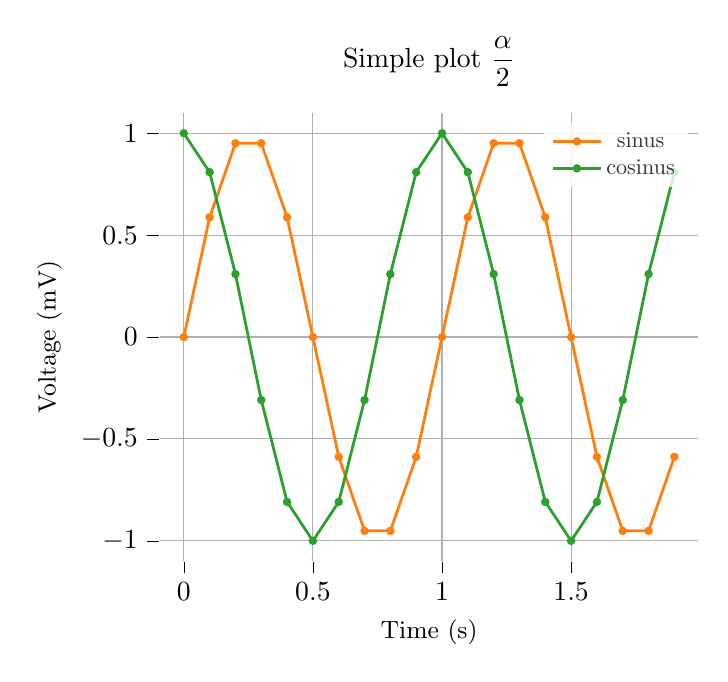
\begin{tikzpicture}



\begin{axis}[
axis line style={white},
tick align=outside,
tick pos=left,
title={Simple plot \(\dfrac{\alpha}{2}\)},
xlabel={Time (\si{\second})},
xmajorgrids,
xmin=-0.095, xmax=1.995,
ylabel={Voltage (\si{\milli\volt})},
ymajorgrids,
ymin=-1.1, ymax=1.1,
]
\addplot [color0, mark=*]
table {%
0 0
0.1 0.587785252292473
0.2 0.951056516295154
0.3 0.951056516295154
0.4 0.587785252292473
0.5 1.22464679914735e-16
0.6 -0.587785252292473
0.7 -0.951056516295154
0.8 -0.951056516295154
0.9 -0.587785252292473
1 -2.44929359829471e-16
1.1 0.587785252292474
1.2 0.951056516295154
1.3 0.951056516295154
1.4 0.587785252292473
1.5 3.67394039744206e-16
1.6 -0.587785252292473
1.7 -0.951056516295154
1.8 -0.951056516295154
1.9 -0.587785252292473
};
\addlegendentry{sinus}
\addplot [color1, mark=*]
table {%
0 1
0.1 0.809016994374947
0.2 0.309016994374947
0.3 -0.309016994374948
0.4 -0.809016994374947
0.5 -1
0.6 -0.809016994374947
0.7 -0.309016994374948
0.8 0.309016994374947
0.9 0.809016994374947
1 1
1.1 0.809016994374947
1.2 0.309016994374947
1.3 -0.309016994374947
1.4 -0.809016994374947
1.5 -1
1.6 -0.809016994374948
1.7 -0.309016994374946
1.8 0.309016994374947
1.9 0.809016994374947
};
\addlegendentry{cosinus}
\end{axis}

\end{tikzpicture}

    \caption{Caption}
    \label{fig:my_label}
\end{figure}


\chapter{Rationale en doelstelling}\label{ch:introduction}

Sinds de introductie van de \gls{led} is de verlichtingswereld sterk veranderd. In vergelijking met traditionele verlichtingstechnologie\"en zijn \gls{led}s kleine en effici\"ente lichtbronnen. \gls{led}s kunnen verschillende kleuren produceren door basiskleuren te combineren, maar het is moeilijk om effici\"ent kleuren zoals wit te maken. Om dit te bereiken, gebruikt men luminescente materialen zoals fosforen, waarmee men op een effici\"ente manier \gls{led}s in deze kleuren kan cre\"eren. Daarnaast moeten \gls{led}s voldoen aan specifieke kleurweergave-eisen.

Belangrijke begrippen zoals kleur en kleurweergave spelen hierbij een rol. Deze begrippen, de werking van \gls{led}s en de effecten van verschillende factoren zijn echter moeilijk intu\"itief te begrijpen.

Om het aanleren van deze concepten te vergemakkelijken, wordt in deze thesis een educatieve \gls{led} webapp ontwikkeld. In deze app kunnen gebruikers experimenteren met verschillende waarden, \gls{led}s, luminescente materialen, enzovoort, en op een experimentele manier leren over de effecten hiervan.

\section{Bestaande tools}

Er bestaan natuurlijk al tools die vergelijkbare functionaliteiten bieden als die wij in de app willen implementeren. Daarom hebben wij verschillende tools onderzocht en gekeken hoe zij deze functionaliteiten realiseren.

\subsection{Waveform lighting}

Op de website van Waveform Lighting zijn enkele eenvoudige webapps te vinden voor het berekenen van de \gls{spd}, chromaticiteit en de \gls{cri}. Twee van hun beste tools zijn de ``LED Spectrum Simulator'' en de ``Color Rendering Index Calculator''. Deze tools zijn echter op een vrij simpele manier ontworpen. In de spectrum simulator kan de gebruiker bijvoorbeeld alleen het vermogen van vier \gls{led}s met een vast profiel aanpassen. Dit beperkt de mogelijkheid om verschillende combinaties van \gls{led}s uit te proberen en staat dus minder experimentatie toe. De color rendering index calculator biedt wat meer vrijheid, maar is minder gebruiksvriendelijk. De gebruiker moet namelijk alle 401 vermogenswaarden van 380 \gls{nm} tot 780 \gls{nm} handmatig invoeren om de \gls{cri} te berekenen. Bovendien is het bij deze tools minder handig dat deze allemaal apart zijn. Het is dus niet mogelijk om een \gls{spd} te maken en hiervan het effect op chromaticiteit, \gls{cri}, enzovoort te zien. Het zijn echter wel makkelijk te vinden tools die vrij makkelijk te gebruiken zijn. 

\begin{figure}[H]
    \centering
    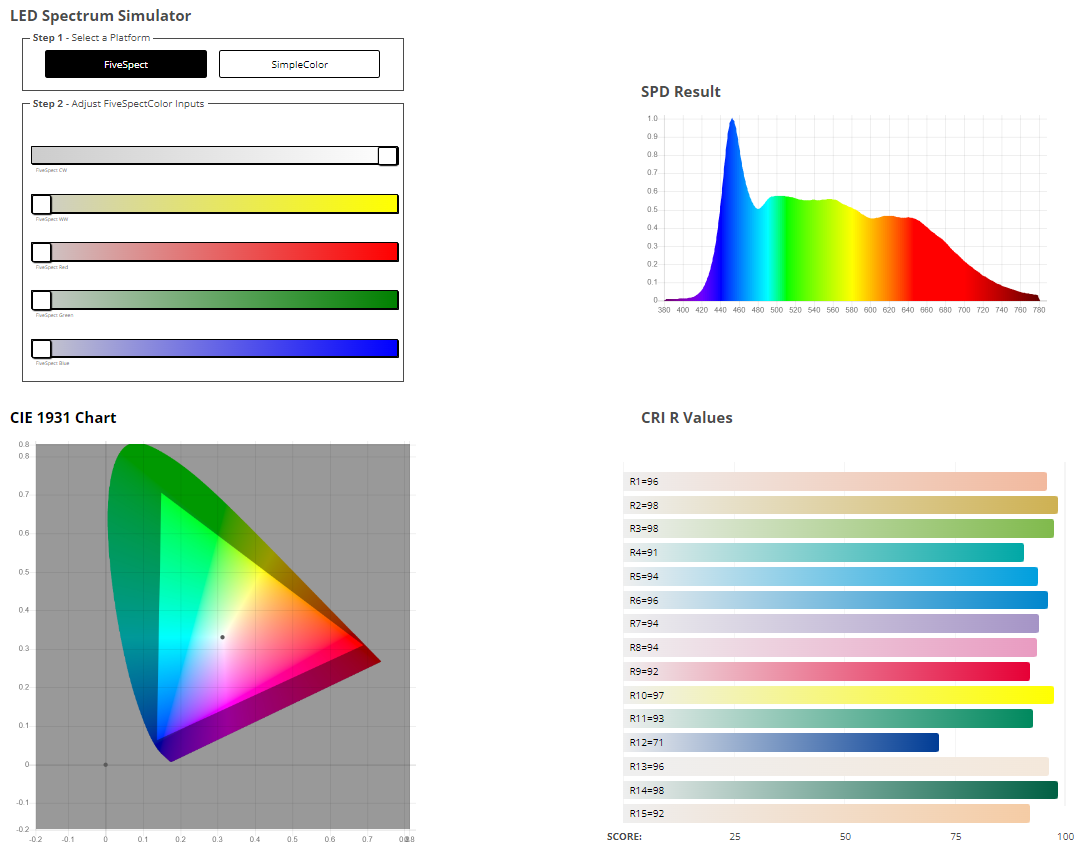
\includegraphics[width=0.95\linewidth]{figs/waveform_spectral.png}
    \caption{Waveform lighting spectrum simulator ~\cite{LEDSpectrumSimulator}}%
    \label{fig:spectrum simulator}
\end{figure}

\subsection{OSRAM ColorCalculator}

De OSRAM ColorCalculator applicatie is een tool die bedoeld is voor het ontwikkelen van ``color mixing \gls{led} lighting solutions''. De software heeft twee hoofdmodi: een ''General photometry'' mode en een ''optimization'' mode. Net als de ''LED Spectrum Simulator'' tool van Waveform Lighting bevat het een chromaticity diagram, \gls{cri}-waarden en een \gls{spd} diagram. Daarnaast biedt het een reeks andere plots, zoals L*a*b*, Delta(u,v), enzovoort. Deze plots zijn echter moeilijker te vinden. Het grootste probleem van de OSRAM ColorCalculator applicatie is echter de drukke \gls{ui}, die de tool moeilijk bruikbaar maakt. Dit zorgt ervoor dat dit een tool is die minder geschikt is voor een lerende gebruiker. Bovendien heeft de applicatie, net als de Waveform Lighting tools, geen mogelijkheid om vrij een \gls{led} toe te voegen met een golflengte tussen 380 nm en 780 nm. Gebruikers moeten \gls{led}s toevoegen met golflengtes in een specifiek bereik. Het grootste probleem is echter dat de applicatie moeilijk te vinden is. Alle downloads op de website van OSRAM zijn verwijderd, en de enige plaats waar de applicatie nog beschikbaar is, is bij de paper op ResearchGate~\cite{selverianColorCalculatorSoftware2017}. Dit maakt het moeilijk voor een gebruiker om de tool te vinden en te gebruiken.

\begin{figure}[H]
    \centering
    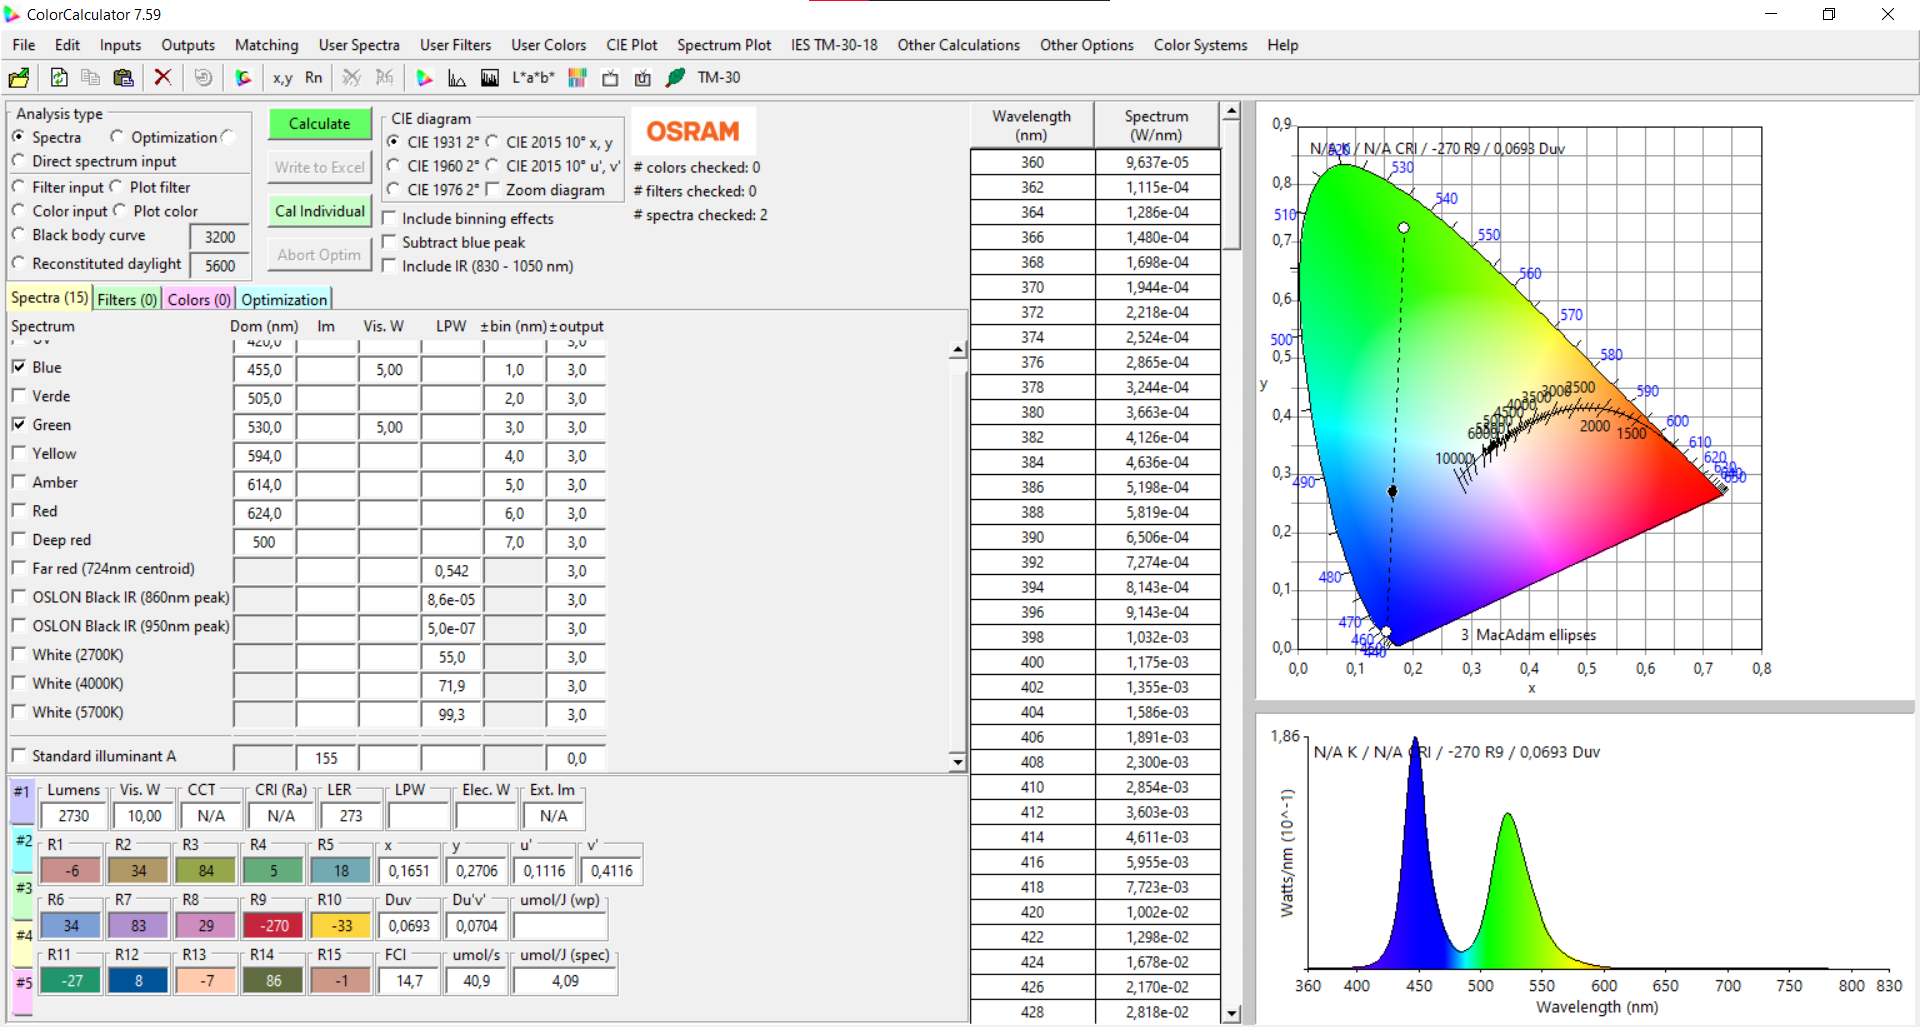
\includegraphics[width=0.95\linewidth]{figs/OSRAM_colorcalculator.png}
    \caption{OSRAM ColorCalculator ~\cite{selverianColorCalculatorSoftware2017}}%
    \label{fig:OSRAM ColorCalculator}
\end{figure}

\subsection{Excel KU Leuven}

Binnen de richting Ingenieurswetenschappen aan KU Leuven Gent wordt een Excel-bestand gebruikt. Dit bestand biedt de mogelijkheid om vier \gls{led}s en twee fosforen in te stellen. Het bevat grafieken van de \gls{spd}, de chromaticiteit, de \gls{eqe} van de \gls{led}s en een color view (met de \gls{cri}). Deze tool is echter niet erg gebruiksvriendelijk, aangezien de gebruiker alle waarden handmatig moet invoeren. Dit maakt het moeilijk voor de gebruiker om met waarden te experimenteren en de effecten daarvan te zien. Bovendien wordt experimenteren bemoeilijkt doordat de resultaten en de inputs zich op verschillende tabbladen bevinden. Ten slotte is deze Excel alleen beschikbaar voor studenten van KU Leuven die het vak volgen waarin deze wordt gebruikt.

\subsection{Conclusie}

Er zijn dus al enkele tools beschikbaar die vergelijkbare functionaliteiten bieden. Deze tools zijn echter te simpel, te ongebruiksvriendelijk en moeilijk te vinden. Bovendien zijn er geen tools die functionaliteit voor luminescente materialen zoals fosforen en quantum dots aanbieden. Het is dus zeker een goed idee om een gebruiksvriendelijke, gemakkelijk te vinden webapp te ontwikkelen die deze functionaliteiten implementeert. De grootste voordelen van onze webapp zijn dus de vrijheid van gebruik en de simulatie van luminescente materialen. Daarnaast bied de app een grotere mogelijkheid tot experimenteren.






\chapter{Relevante Concepten}\label{ch:concepten}

In dit hoofdstuk leggen we alle concepten uit die nodig zijn om de volledige functionaliteit van de webapp te begrijpen.

Dit hoofdstuk is hoofdzakelijk gebaseerd op ~\cite{LightingTechnologyHandbook,InteriorLightingHandbook,Light-EmittingDiodes,FundamentalsofSolidStateLighting}

\section{Spectral power distribution}{\label{sec:spectral-power-distribution}}

De \gls{spd} is een essentieel concept voor het gebruik van de app en de verschillende berekeningen die hierin worden uitgevoerd. Het vormt de basis voor alle andere berekeningen. Bovendien maakt de \gls{spd} het eenvoudig om experimentele aanpassingen snel te visualiseren. Aan de hand van de \gls{spd} kunnen we per golflengte zien hoeveel optische straling wordt uitgezonden. Het wordt gedefinieerd als de hoeveelheid optische straling die door een bron wordt uitgezonden binnen een smalle band $\Delta\lambda$, gecentreerd rond een specifieke golflengte $\lambda$. Door een grafiek van de spectral power distribution te maken, kunnen we bijvoorbeeld zien bij welke golflengte een \gls{led} de grootste optische straling heeft en welk effect het toevoegen van luminescente materialen heeft.

\begin{figure}[H]
    \centering
    \resizebox{0.7\textwidth}{!}{% This file was created with tikzplotlib v0.10.1.
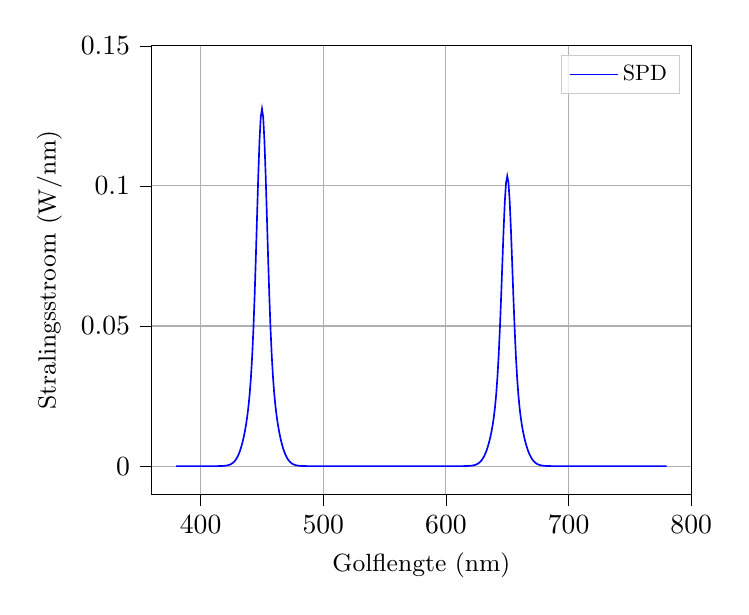
\begin{tikzpicture}

\definecolor{darkgray176}{RGB}{176,176,176}
\definecolor{lightgray204}{RGB}{204,204,204}

\begin{axis}[
legend cell align={left},
legend style={fill opacity=0.8, draw opacity=1, text opacity=1, draw=lightgray204},
tick align=outside,
tick pos=left,
x grid style={darkgray176},
xlabel={Golflengte (nm)},
xmajorgrids,
xmin=360, xmax=800,
xtick style={color=black},
y grid style={darkgray176},
ylabel={Stralingsstroom (W/nm)},
ymajorgrids,
ymin=-0.01, ymax=0.15,
yticklabels={-0.01, 0, 0.05, 0.1, 0.15},
ytick style={color=black}
]
\addplot [semithick, blue]
table {%
380 1.02073728218891e-15
381 2.48463356981015e-15
382 5.9710643336564e-15
383 1.41671399063567e-14
384 3.31859034825859e-14
385 7.67478360943115e-14
386 1.75234520140434e-13
387 3.95015573955344e-13
388 8.79123327229562e-13
389 1.9316410234851e-12
390 4.19028986979639e-12
391 8.97434465598681e-12
392 1.89759030340542e-11
393 3.96134977666599e-11
394 8.16441290421166e-11
395 1.66129883456256e-10
396 3.33742558513386e-10
397 6.61936687321886e-10
398 1.29617112990747e-09
399 2.5058165109343e-09
400 4.78274492556851e-09
401 9.01251920821373e-09
402 1.67670329461642e-08
403 3.07969184267533e-08
404 5.58469343871304e-08
405 9.99844460004153e-08
406 1.76728495979833e-07
407 3.08405240440691e-07
408 5.3134665042051e-07
409 9.03805908085318e-07
410 1.51779610976949e-06
411 2.51647560939047e-06
412 4.11920158656256e-06
413 6.65693624151611e-06
414 1.06212780781283e-05
415 1.67309342278416e-05
416 2.60198408056627e-05
417 3.99512257927416e-05
418 6.05614986236792e-05
419 9.06367132931326e-05
420 0.000133922242960297
421 0.000195362997908766
422 0.000281366856992435
423 0.000400077936995756
424 0.000561639068050377
425 0.00077841482796926
426 0.00106513852909163
427 0.00143893996057875
428 0.00191920760002315
429 0.00252724323990337
430 0.00328568613450886
431 0.00421773351462523
432 0.00534629488383525
433 0.0066934389805901
434 0.00828088606531231
435 0.0101328895377022
436 0.0122835132371137
437 0.0147905861658002
438 0.0177575796773932
439 0.0213610811858614
440 0.0258747153599907
441 0.0316715457905161
442 0.0391807935798618
443 0.0487787235769689
444 0.0606145246750115
445 0.0744090729810278
446 0.0893035494803108
447 0.103850903364327
448 0.116213345545371
449 0.124551928022846
450 0.1275
451 0.124551928022846
452 0.116213345545371
453 0.103850903364327
454 0.0893035494803108
455 0.0744090729810278
456 0.0606145246750115
457 0.0487787235769689
458 0.0391807935798618
459 0.0316715457905161
460 0.0258747153599907
461 0.0213610811858614
462 0.0177575796773932
463 0.0147905861658002
464 0.0122835132371137
465 0.0101328895377022
466 0.00828088606531231
467 0.0066934389805901
468 0.00534629488383525
469 0.00421773351462523
470 0.00328568613450886
471 0.00252724323990337
472 0.00191920760002315
473 0.00143893996057875
474 0.00106513852909163
475 0.00077841482796926
476 0.000561639068050377
477 0.000400077936995756
478 0.000281366856992435
479 0.000195362997908766
480 0.000133922242960297
481 9.06367132931326e-05
482 6.05614986236792e-05
483 3.99512257927416e-05
484 2.60198408056627e-05
485 1.67309342278416e-05
486 1.06212780781283e-05
487 6.65693624151611e-06
488 4.11920158656256e-06
489 2.51647560939047e-06
490 1.51779610976949e-06
491 9.03805908085318e-07
492 5.3134665042051e-07
493 3.08405240440691e-07
494 1.76728495979833e-07
495 9.99844460004153e-08
496 5.58469343871304e-08
497 3.07969184267533e-08
498 1.67670329461642e-08
499 9.01251920821373e-09
500 4.78274492556851e-09
501 2.5058165109343e-09
502 1.29617112990747e-09
503 6.61936687321886e-10
504 3.33742558513386e-10
505 1.66129883456256e-10
506 8.16441290421166e-11
507 3.96134977666599e-11
508 1.89759030340542e-11
509 8.97434465598681e-12
510 4.19028986979639e-12
511 1.9316410234851e-12
512 8.79123327229562e-13
513 3.95015573955344e-13
514 1.75234520140434e-13
515 7.67478360943115e-14
516 3.31859034825859e-14
517 1.41671399063567e-14
518 5.9710643336564e-15
519 2.48463356981015e-15
520 1.02073728218891e-15
521 4.14006001808021e-16
522 1.65783127084198e-16
523 6.55412995118465e-17
524 2.55817823406707e-17
525 9.85797202853517e-18
526 3.75046739484557e-18
527 1.40871856334676e-18
528 5.22401134581402e-19
529 1.91260380780255e-19
530 6.91332464117623e-20
531 2.46711797298917e-20
532 8.69228412377663e-21
533 3.02356243317445e-21
534 1.0383529437434e-21
535 3.52056272826524e-22
536 1.17847454399517e-22
537 3.89465825401622e-23
538 1.27074829524738e-23
539 4.09346184454742e-24
540 1.30185611745346e-24
541 4.08767407257552e-25
542 1.26715739841099e-25
543 3.87816160492372e-26
544 1.17182385798815e-26
545 3.49575211123742e-27
546 1.02960506615758e-27
547 2.99488653307453e-28
548 8.63614143122872e-29
549 2.58876117231654e-29
550 1.23493438572245e-29
551 2.16568468807202e-29
552 7.02803073593441e-29
553 2.43161485622973e-28
554 8.35809593355053e-28
555 2.83773147575922e-27
556 9.51245334716413e-27
557 3.14815473640599e-26
558 1.02863365337891e-25
559 3.31822954140463e-25
560 1.05680084828914e-24
561 3.32292785028049e-24
562 1.03154861614201e-23
563 3.16154611208376e-23
564 9.56644041596078e-23
565 2.85786856765061e-22
566 8.42898271979936e-22
567 2.45442126928279e-21
568 7.05608946518338e-21
569 2.00271929572062e-20
570 5.61199294401365e-20
571 1.55258426751031e-19
572 4.24066803366079e-19
573 1.14354801024619e-18
574 3.04449706169817e-18
575 8.00235376434031e-18
576 2.0766388017721e-17
577 5.32041137213813e-17
578 1.34576891397761e-16
579 3.36075460291217e-16
580 8.28598499659234e-16
581 2.01693783902236e-15
582 4.84709928261519e-15
583 1.15003841592778e-14
584 2.69391451799815e-14
585 6.23011845942058e-14
586 1.42249198702234e-13
587 3.20659701210809e-13
588 7.13641289162821e-13
589 1.56803800729967e-12
590 3.40152942371707e-12
591 7.285056250154e-12
592 1.5403968345291e-11
593 3.21568393635239e-11
594 6.62758223988946e-11
595 1.34858375982137e-10
596 2.70920429852043e-10
597 5.3733684029659e-10
598 1.05218597604254e-09
599 2.03413340299373e-09
600 3.88246352781444e-09
601 7.31604500431467e-09
602 1.36108855680627e-08
603 2.49998514287762e-08
604 4.53345702672e-08
605 8.11638444003371e-08
606 1.434619555601e-07
607 2.50352489298914e-07
608 4.31328457400179e-07
609 7.33677737151611e-07
610 1.23209331263641e-06
611 2.04278608291697e-06
612 3.34382246438607e-06
613 5.4038658901719e-06
614 8.62197867518649e-06
615 1.35815819026009e-05
616 2.11219884187144e-05
617 3.24309950552843e-05
618 4.91616871180454e-05
619 7.35756849085429e-05
620 0.00010871335016777
621 0.000158588786537704
622 0.000228403683911506
623 0.000324769148855378
624 0.000455918772887953
625 0.000631889683880929
626 0.000864641864792028
627 0.00116808067388157
628 0.00155794499295996
629 0.00205152686533332
630 0.00266720403860131
631 0.00342380720598989
632 0.00433993349393685
633 0.0054334975254202
634 0.00672213104125353
635 0.00822552209531119
636 0.00997132251012758
637 0.0120064758287084
638 0.0144149764440015
639 0.0173401717861699
640 0.0210041807039924
641 0.0257098430534777
642 0.0318055853765937
643 0.0395968461977747
644 0.0492047317950094
645 0.0604026592434226
646 0.0724934695781347
647 0.0843024980251592
648 0.0943378922662423
649 0.101106859218545
650 0.1035
651 0.101106859218545
652 0.0943378922662423
653 0.0843024980251592
654 0.0724934695781347
655 0.0604026592434226
656 0.0492047317950094
657 0.0395968461977747
658 0.0318055853765937
659 0.0257098430534777
660 0.0210041807039924
661 0.0173401717861699
662 0.0144149764440015
663 0.0120064758287084
664 0.00997132251012758
665 0.00822552209531119
666 0.00672213104125353
667 0.0054334975254202
668 0.00433993349393685
669 0.00342380720598989
670 0.00266720403860131
671 0.00205152686533332
672 0.00155794499295996
673 0.00116808067388157
674 0.000864641864792028
675 0.000631889683880929
676 0.000455918772887953
677 0.000324769148855378
678 0.000228403683911506
679 0.000158588786537704
680 0.00010871335016777
681 7.35756849085429e-05
682 4.91616871180454e-05
683 3.24309950552843e-05
684 2.11219884187144e-05
685 1.35815819026009e-05
686 8.62197867518649e-06
687 5.4038658901719e-06
688 3.34382246438607e-06
689 2.04278608291697e-06
690 1.23209331263641e-06
691 7.33677737151611e-07
692 4.31328457400179e-07
693 2.50352489298914e-07
694 1.434619555601e-07
695 8.11638444003371e-08
696 4.53345702672e-08
697 2.49998514287762e-08
698 1.36108855680627e-08
699 7.31604500431467e-09
700 3.88246352781444e-09
701 2.03413340299373e-09
702 1.05218597604254e-09
703 5.3733684029659e-10
704 2.70920429852043e-10
705 1.34858375982137e-10
706 6.62758223988946e-11
707 3.21568393635239e-11
708 1.5403968345291e-11
709 7.285056250154e-12
710 3.40152942371707e-12
711 1.56803800729967e-12
712 7.13641289162821e-13
713 3.20659701210809e-13
714 1.42249198702234e-13
715 6.23011845942058e-14
716 2.69391451799815e-14
717 1.15003841592778e-14
718 4.84709928261519e-15
719 2.01693783902236e-15
720 8.28598499659234e-16
721 3.36075460291217e-16
722 1.34576891397761e-16
723 5.32041137213813e-17
724 2.0766388017721e-17
725 8.00235376434031e-18
726 3.04449706169817e-18
727 1.14354801024619e-18
728 4.24066803366079e-19
729 1.55258426751031e-19
730 5.61199294401365e-20
731 2.00271929572062e-20
732 7.05608946518338e-21
733 2.45442126928279e-21
734 8.42898271979936e-22
735 2.85786856765061e-22
736 9.56644041596078e-23
737 3.16154611208374e-23
738 1.03154861614195e-23
739 3.32292785027808e-24
740 1.05680084827921e-24
741 3.31822954100161e-25
742 1.02863365176276e-25
743 3.14815467242237e-26
744 9.51245084624862e-27
745 2.83772182480431e-27
746 8.35772824290086e-28
747 2.43023181248878e-28
748 6.97667011378765e-29
749 1.97737803397955e-29
750 5.5331475723928e-30
751 1.52860695675071e-30
752 4.16927403308985e-31
753 1.12270609559045e-31
754 2.98478292084364e-32
755 7.83430458099105e-33
756 2.0301549371465e-33
757 5.19396412834549e-34
758 1.31192720744546e-34
759 3.27161026619249e-35
760 8.05479360303098e-36
761 1.95789005890491e-36
762 4.69854311830356e-37
763 1.113215290091e-37
764 2.60397097723442e-38
765 6.01359459342634e-39
766 1.37111279851383e-39
767 3.08640741245433e-40
768 6.85921399929498e-41
769 1.50499993921338e-41
770 3.26016546688947e-42
771 6.97242472027366e-43
772 1.47220760121888e-43
773 3.06898883240684e-44
774 6.31629770153123e-45
775 1.28342621172719e-45
776 2.57466215297901e-46
777 5.09930071577513e-47
778 9.97107606827849e-48
779 1.92492789283254e-48
780 3.66883290430096e-49
};
\addlegendentry{SPD}
\end{axis}

\end{tikzpicture}
}
    \caption{Voorbeeld spectral power distribution}
    \label{fig:VBSPD}
\end{figure}

\section{External quantum efficiency}{\label{sec:external-quantum-efficiency}}

Het volgende belangrijke concept is de \gls{eqe}. Dit begrip geeft aan hoeveel fotonen er voor de inkomende elektronen de \gls{led} verlaten. Dit is cruciaal bij het berekenen van de spectral power distribution van een \gls{led}. Afhankelijk van de centrale golflengte kan de external quantum efficiency namelijk sterk vari\"eren. Dit zorgt ervoor dat de hoeveelheid stralingsstroom voor bepaalde \gls{led}s een stuk kleiner is, doordat minder fotonen de \gls{led} kunnen verlaten. Zo hebben bijvoorbeeld groene \gls{led}s een veel lagere effici\"entie dan andere \gls{led}s (the green gap ~\cite{ExternalQuantumEfficiency,hahnClosingGreenGapb,FrontiersEQE,zhuSolidStateLightingBased2016EQE}), wat ervoor zorgt dat deze \gls{led}s meer vermogen nodig hebben. Het effect van de \gls{eqe} is rechtstreeks af te lezen in de spectral power distribution. Zo zal een groene \gls{led} met hetzelfde ingangsvermogen als een blauwe \gls{led} minder licht produceren.

\section{Chromaticiteit}\label{sec:chromaticiteit}

Door de verschillende \gls{spd}s van lichtbronnen ontstaat voor de mens een bepaalde kleur. Om te bepalen met welke kleur een \gls{spd} overeenkomt, maken we gebruik van een chromaticiteitsdiagram. Dit diagram helpt ons de kleur te visualiseren die wordt waargenomen op basis van de \gls{spd} van een lichtbron. Om op het chromaticiteitsdiagram tot een kleur te komen, moeten we eerst gebruik maken van de $\bar{x}(\lambda), \, \bar{y}(\lambda), \, \text{en} \, \bar{z}(\lambda)$ \gls{cmf} en de X, Y en Z tristimuluswaarden.

De \gls{cmf} (colour matching functions) zijn numerieke waarden die de chromatische respons van de waarnemer beschrijven. Chromatische respons betekent de manier waarop het menselijk oog verschillende golflengten van licht (kleuren) waarneemt. Het menselijk oog is namelijk gevoelig voor verschillende golflengtes, en de \gls{cmf} geven aan hoe sterk het oog reageert op licht bij verschillende golflengtes. Dit zijn als het ware de "gevoeligheidsfuncties" voor de verschillende kleuren die we kunnen waarnemen.

De X, Y en Z tristimuluswaarden zijn net zoals de RGB-waarden (rood, groen, blauw) een manier om een kleur voor te stellen, maar ze zijn gebaseerd op hoe een gemiddeld menselijk oog reageert op licht. De tristimuluswaarden X, Y en Z geven een gestandaardiseerde manier om de kleur van een lichtbron te berekenen op basis van de waarneming van de mens.

De waarnemer die we gebruiken om de \gls{cmf} te berekenen, is gebaseerd op de chromatische respons van een gemiddelde mens, die een respons heeft binnen een boog van twee graden van het gezichtsveld. Dit model wordt gebruikt omdat het menselijk zicht niet overal in het gezichtsveld even gevoelig is voor kleur. De \gls{cmf}s kunnen we dan zien als de spectrale "intensiteit" curves van drie lichtdetectoren, die samen de CIE-tristimuluswaarden X, Y en Z opleveren.

Aan de hand van de \gls{cmf} en de \gls{spd} van de te analyseren lichtbron kunnen we de X, Y en Z waarden berekenen op de volgende manier ~\cite{LightingTechnologyHandbook, CIE1931ColorSpace2024}:

\begin{align*}
X &= k.\int_{\lambda} \bar{x}(\lambda) P(\lambda) \, d\lambda \\
Y &= k.\int_{\lambda} \bar{y}(\lambda) P(\lambda) \, d\lambda \\
Z &= k.\int_{\lambda} \bar{z}(\lambda) P(\lambda) \, d\lambda
\end{align*}

Met $P(\lambda)$ de \gls{spd} van de lichtbron en $k$ een normalisatieconstante.

Aan de hand van deze tristimulus waarden kunnen vervolgens de chromaticiteitsco\"ordinaten berekend worden.

\begin{align*}
x &= \frac{X}{X + Y + Z} \\
y &= \frac{Y}{X + Y + Z} \\
z &= \frac{Z}{X + Y + Z}
\end{align*}

Conventioneel worden de x- en y-co\"ordinaten in het chromaticiteitsdiagram gebruikt om een punt of kleur aan te duiden. Het is belangrijk om te begrijpen dat deze co\"ordinaten niet bedoeld zijn om een specifieke kleur vast te leggen, maar om de kleur te situeren. Dit komt doordat het chromaticiteitsdiagram enkel rekening houdt met de tint (hue) en verzadiging (saturation), maar niet met de lichtheid. Toch kunnen de chromaticiteitsco\"ordinaten verder worden gebruikt om de \gls{cct} en \gls{cri} waarden te berekenen.

\begin{figure}[H]
    \centering
    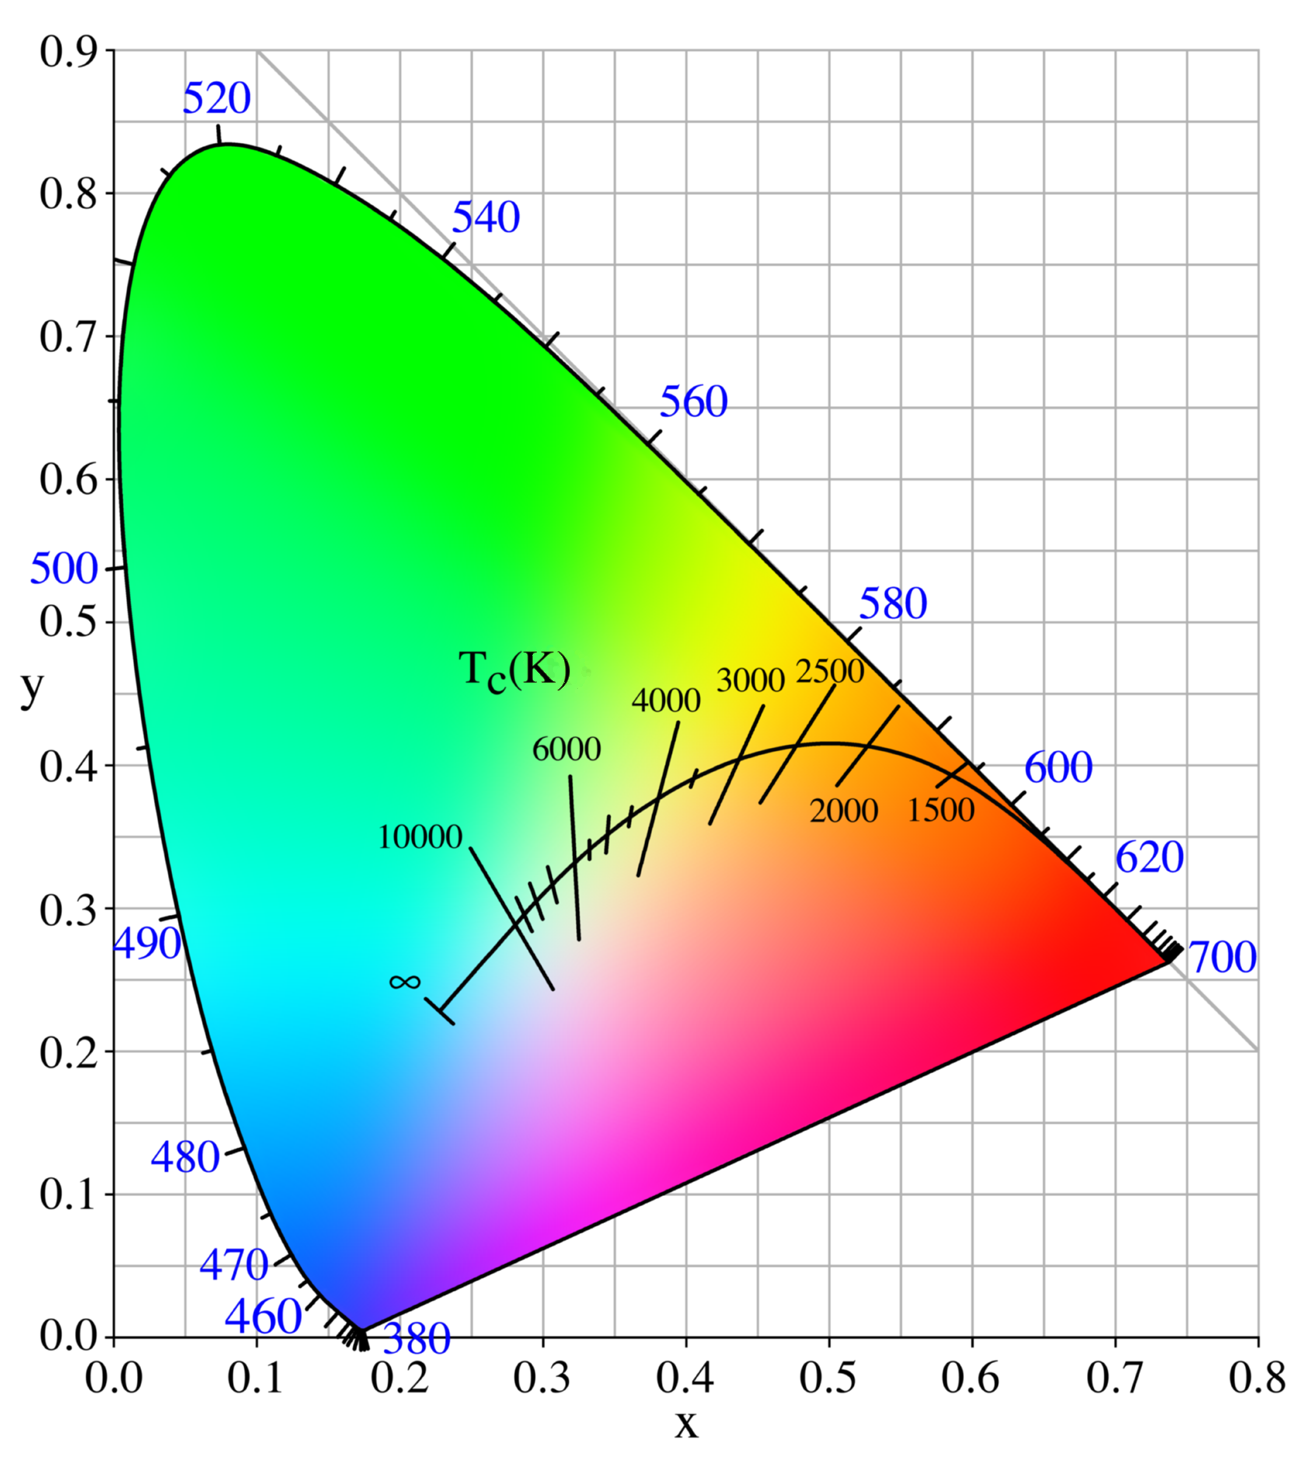
\includegraphics[width=0.6\linewidth]{figs/PlanckianLocus.png}
    \caption{Chromaticiteitsdiagram ~\cite{Chromaticiteit2017}}%
    \label{fig:chromaticiteitsdiagram}
\end{figure}

\subsection{Correlated color temperature}

Een andere belangrijke waarde bij de chromaticiteit is de \gls{cct}. De \gls{cct} is een maat voor de kleur van een lichtbron aan de hand van een temperatuur. Deze maat is gebaseerd op temperaturen bij ''blackbody radiators''. Een ''blackbody radiator'' is een object dat alle invallende straling absorbeert en vervolgens weer uitzendt.

Bij een ''blackbody radiator'' is de kleur volledig afhankelijk van de temperatuur. Hierdoor kunnen we de temperatuur van een ''blackbody radiator'' gebruiken om zijn kleur te beschrijven. Zo bevindt een witte ''blackbody radiator'' zich bijvoorbeeld rond 5000 K.

We kunnen de ''Color temperature'' linken met de chromaticiteit aan de hand van de curve in \cref{fig:chromaticiteitsdiagram}. Deze curve wordt de ''blackbody locus'' of blackbody curve genoemd en stelt de kleur voor van ''blackbody radiators'' bij verschillende temperaturen.

Wanneer de chromaticiteit van een lichtbron op de ''blackbody locus'' ligt, kan de ''Color temperature'' gegeven worden. Ligt de chromaticiteit van een lichtbron echter niet op de ''blackbody locus'', dan kan deze waarde niet worden gebruikt. In dit geval wordt de \gls{cct} waarde gebruikt, die de temperatuur van een ''blackbody radiator'' weergeeft die ongeveer dezelfde kleur heeft als de lichtbron.

\section{Color rendering index}

De \gls{cri} is een maat voor hoe goed een lichtbron kleuren kan weergeven ~\cite{ColorRenderingLight,LightingTechnologyHandbook}. Het is een getal tussen 0 en 100, waarbij 100 de beste kleurweergave voorstelt. De \gls{cri} wordt berekend aan de hand van de kleurweergave van 8 of meer testkleuren.

De \gls{cri} waarde wordt bepaald door de kleursverandering van een testkleur onder de lichtbron te vergelijken met de kleursverandering van de testkleur onder een referentie lichtbron. Van elke van deze 8 of meer kleuren wordt de $R_i$ waarde berekend, wat de kleurverandering van de testkleur onder de lichtbron aangeeft in vergelijking met de referentiebron. Aan de hand van deze $R_i$ waarden wordt een gemiddelde berekend, de \gls{cri} waarde. 

In de standaardmethode is de referentiebron een black body radiator wanneer de \gls{cct} van de lichtbron kleiner is dan 5000K. Is de \gls{cct} groter dan 5000K, dan wordt een mathematisch model van daglicht gebruikt als referentiebron. Naast de acht standaardkleuren kunnen er ook zes extra kleuren optioneel worden toegevoegd. Deze kleuren verbeteren de nauwkeurigheid van de \gls{cri} waarde. 

Van deze extra kleuren is $R_9$ een zeer belangrijke ~\cite{WhatCRIR9}. Lichtbronnen met een lage $R_9$ waarde worden namelijk vaak als onaangenaam ervaren. Dit komt doordat de testkleur voor $R_9$ een rode kleur is, die belangrijk is voor de weergave van bijvoorbeeld huidskleur. Veel lichtbronnen stralen minder licht uit bij de rode golflengtes, waardoor de $R_9$ waarde vaak laag is. Dit is echter niet zichtbaar in de standaard \gls{cri} waarde.

De \gls{cri} waarde is belangrijk voor het beoordelen van de kwaliteit van een lichtbron, maar het is niet altijd de beste maatstaf. De \gls{cri} is niet in staat om lichtbronnen goed te rangschikken, vooral niet wanneer \gls{led}s worden gebruikt. Dit komt door de dunne emissiespectra van \gls{led}s, waarin het licht wordt gemengd. Voor deze reden worden nog andere methodes gebruikt/ontwikkeld om de kleurweergave van lichtbronnen te beoordelen. Het is belangrijk dat deze methodes worden gebruikt als een hulp bij het beoordelen van de kwaliteit van een lichtbron en niet als enige maatstaf.

\subsection{Berekening CRI\texorpdfstring{~\cite{rootPrincipleBasicCalculation,ColorRenderingIndexWiki}}{}}

In de standaardberekening van de \gls{cri} waarde wordt de ''color rendering'' van de testbron vergeleken met die van een referentiebron. Zoals eerder vermeld, wordt een black body radiator als referentiebron gebruikt wanneer de \gls{cct} van de testbron kleiner is dan 5000K. Is de \gls{cct} groter dan 5000K, dan wordt een mathematisch model van daglicht gebruikt.

De berekening begint met het bepalen van de x,y-co\"ordinaten van de testbron. Deze co\"ordinaten worden omgezet naar u,v-co\"ordinaten. De u,v-co\"ordinaten zijn een andere manier om kleuren te representeren en worden vaak gebruikt in kleurwetenschap vanwege hun perceptuele uniformiteit. De u,v-co\"ordinaten worden vervolgens gebruikt om de \gls{cct} te berekenen door het dichtstbijzijnde punt op de Planckian locus te vinden. Aan de hand van deze \gls{cct} waarde wordt de referentiebron bepaald.

Daarna wordt de afstand van de testbron tot de Planckian locus (DC) berekend. Dit geeft aan of het resultaat relevant is. De \gls{cri} waarde is namelijk enkel gedefinieerd voor lichtbronnen die ongeveer wit zijn.

% formula of DC
\begin{align*}
    DC = \sqrt{(u - u_{\text{Planckian}})^2 + (v - v_{\text{Planckian}})^2}
\end{align*}

Als de waarde van DC boven $5.4 \times 10^{-3}$ ligt, is de \gls{cri} waarde niet relevant.

Vervolgens worden de testsamples belicht met zowel de testbron als de referentiebron. Aan de hand hiervan worden de u,v-co\"ordinaten van het licht dat door de testsamples gereflecteerd wordt, bepaald. Daarna wordt op elk van deze samples een von Kries-transformatie toegepast. Dit is een transformatie die wordt uitgevoerd om rekening te houden met ''chromatic adaptation''.

''Chromatic adaptation'' is het fenomeen waarbij de gevoeligheid van de ogen verandert om zich aan te passen aan veranderingen in de lichtbron ~\cite{ChromaticAdaptation2023,LightingTechnologyHandbook}. Dit fenomeen zorgt ervoor dat een object onder verschillende belichtingen grotendeels hetzelfde blijft. Zo zal een appel zelfs onder verschillende lichtbronnen nog steeds rood lijken.

De von Kries-transformatie wordt uitgevoerd aan de hand van de volgende formules:

\begin{align}
    c &= \frac{4.0 - u - 10.0v}{v} \\
    d &= \frac{1.708v - 1.481u + 0.404}{v}\\
    u_{c,i} &= \frac{10.872 + 0.404\left(\frac{c_r}{c_t}\right)c_{t,i} - 4\left(\frac{d_r}{d_t}\right)d_{t,i}}{16.518 + 1.481\left(\frac{c_r}{c_t}\right)c_{t,i} - \left(\frac{d_r}{d_t}\right)d_{t,i}} \\
    v_{c,i} &= \frac{5.520}{16.518 + 1.481\left(\frac{c_r}{c_t}\right)c_{t,i} - \left(\frac{d_r}{d_t}\right)d_{t,i}}
\end{align}

Nu kan voor elk sample de euclidische afstand tussen de co\"ordinaten van de testbron en de referentiebron berekend worden. Ten slotte kan de \gls{cri} waarde berekend worden aan de hand van de volgende formule:

\begin{align}
    R_i = 100 - 4.6\Delta E_i
\end{align}

Met $\Delta E_i$ de euclidische afstand tussen de co\"ordinaten van de testbron en de referentiebron voor de $i$-de sample.

Door het nemen van het gemiddelde van de $R_i$ waarden kan de \gls{cri} waarde berekend worden. Het is echter natuurlijk ook belangrijk deze waarden apart te bekijken.

\section[tm30]{tm30\texorpdfstring{\footnote{Gebaseerd op ~\cite{david2018}.}}{}}


Tm30 is een methode voor het evalueren van lichtbronnen die gebruik maakt van een statistische aanpak. Ze stelt zowel algemene eigenschappen (zoals de gamut area) als hue-specifieke eigenschappen (zoals chroma shift, hue shift, ...) voor. Deze methode probeert niet \"e\"en specifieke waarde te geven die de lichtbron evalueert, maar biedt de gebruiker de benodigde kennis om een keuze te maken op basis van zijn of haar ervaring.

De methode maakt gebruik van 99 \gls{ces}, die op statistische wijze werden gekozen uit 100.000 mogelijke \gls{ces}. Om de kleur voor te stellen, maakt de methode gebruik van een groot aantal berekeningen (50). Afhankelijk van de situatie kunnen bepaalde van deze berekeningen worden gebruikt om een keuze te maken. De belangrijkste berekeningen zijn:

\begin{itemize}
    \item Fidelity index ($R_f$)
    \item Gamut index ($R_g$)
    \item Color Vector Graphic (CVG)
    \item Local chroma shift
    \item Local hue shift
\end{itemize}


\subsection{Fidelity index}

De fidelity index is een waarde die aangeeft hoe goed een lichtbron de kleuren van een referentiebron kan weergeven.

De fidelity index van tm30 wordt berekend door de ''CAM02-UCS'' co\"ordinaten van elke \gls{ces} onder de testbron en de referentiebron te berekenen. Vervolgens wordt het rekenkundig gemiddlede genomen, geschaald met een factor 6.73 en afgetrokken van 100.

\begin{align}
    R_f' = 100 - 6.73 \left[ \sum_{i=1}^{9_{19}} 99 \left( \Delta E_{\text{Jab},i} \right) \right]
\end{align}

Met $\Delta E_{\text{Jab},i}$ de euclidische afstand tussen de ''CAM02-UCS'' co\"ordinaten van de testbron en de referentiebron voor de $i$-de \gls{ces}.

Vervolgens wordt nog een aanpassing van de schaal gedaan zodat geen negatieve waarden bekomen worden.

\begin{align}
    R_f = 10 \ln \left[ \exp \left( \frac{R_f'}{10} \right) + 1 \right]
\end{align}

\subsection{Hue-angle bins}

Voor het berekenen van de volgende waarden worden de \gls{ces} in 16 hue-angle bins verdeeld. Deze bins worden dan gebruikt om de volgende waarden te berekenen. De bins worden bepaald door de a'-b' co\"ordinaten van de \gls{ces} in 16 stukken te verdelen volgens een radiaal patroon zoals in \cref{fig:huebins}. Het a'-b' co\"ordinatenstelsel is een kleurruimte die de kleur van een lichtbron voorstelt. De a'-as staat voor de rood-groen as en de b'-as voor de geel-blauw as.

% figure of bins
\begin{figure}[H]
    \centering
    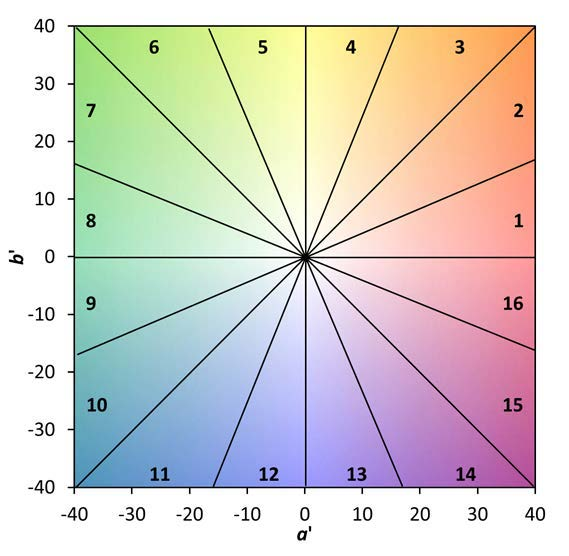
\includegraphics[width=0.6\linewidth]{TM-30-Bins.jpg}
    \caption{Hue-angle bins}%
    \label{fig:huebins}
\end{figure}

\subsection{Gamut (area) index}

De gamut (area) index is een waarde die het gebied aangeeft dat wordt beslagen door de gemiddelde (a', b') co\"ordinaten van de \gls{ces} in elke hue-angle bin. Voor de berekening wordt gewerkt met veelhoeken voor de test- en referentiebron. De gamut index wordt berekend aan de hand van \cref{eq:gamut} met $A_{\text{test}}$ en $A_{\text{ref}}$ als de oppervlakten van de veelhoeken van respectievelijk de test- en referentiebron zoals in \cref{fig:gamut}. ~\cite{david2018,simsWhatGamutArea2022}

\begin{align}
    100 \times \frac{A_{\text{test}}}{A_{\text{ref}}} \label{eq:gamut}
\end{align}

Hiervoor wordt ten eerste voor alle samples het co\"ordinaat van de test en referentiebron berekend zoals in \cref{fig:gamut_samples} voor de testbron te zien is. Vervolgens wordt per bin het gemiddelde van alle test- en referentieco\"ordinaten genomen. Dit levert een veelhoek op voor de test en de referentiebron zoals te zien voor de testbron in \cref{fig:gamut_combined}. Deze veelhoeken worden dan gebruikt om de oppervlakten te berekenen. Aan de hand hiervan kan dan met \cref{eq:gamut} de gamut (area) index berekend worden (\cref{fig:gamut}).

\begin{figure}[H]
    \centering
    \begin{subfigure}[b]{0.45\linewidth}
        \centering
        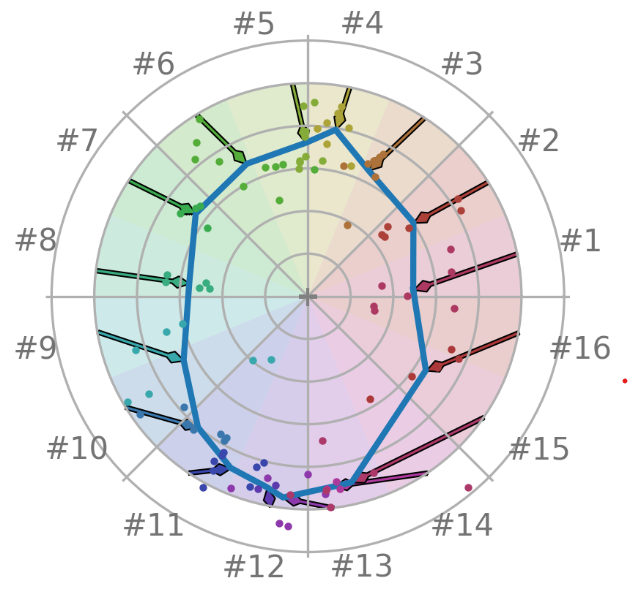
\includegraphics[width=\linewidth]{gamut_samples.png}
        \caption{Test Gamut samples en oppervlak}%
        \label{fig:gamut_samples}
    \end{subfigure}
    \hfill
    \begin{subfigure}[b]{0.45\linewidth}
        \centering
        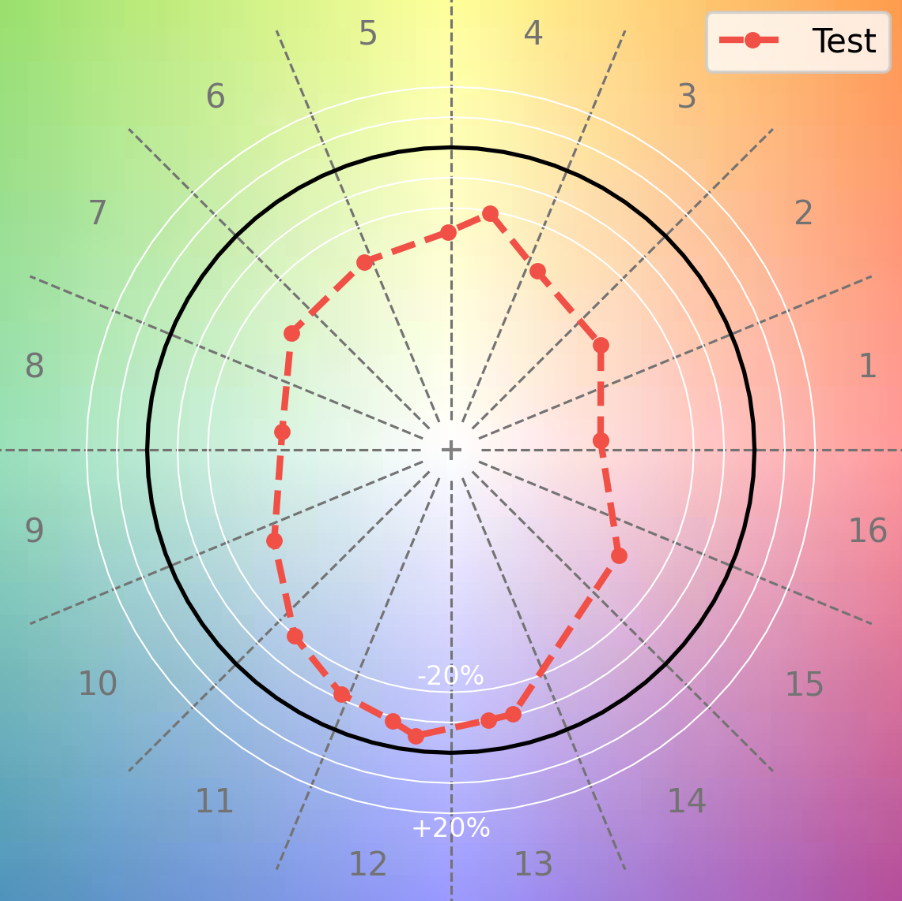
\includegraphics[width=\linewidth]{gamut_index.png}
        \caption{Gamut area index $A_{\text{test}}$ en $A_{\text{ref}}$ (cirkel)}%
        \label{fig:gamut}
    \end{subfigure}
    \caption{Gamut samples (links) en gamut area index (rechts)}%
    \label{fig:gamut_combined}
\end{figure}

\subsection{Color vector graphic}

Een Color Vector Graphic (CVG) laat zien hoe een lichtbron kleuren be\"invloedt. De grafiek toont verschuivingen in kleurintensiteit (chroma) en kleurtint (hue) in een cirkelvormige weergave.

\subsubsection{Chroma (kleurintensiteit)}
\begin{itemize}
    \item Als de lijn van de testlichtbron buiten de referentielijn ligt, worden de kleuren intenser (meer verzadigd).
    \item Ligt de lijn binnen de referentielijn, dan worden de kleuren minder intens (meer dof).
\end{itemize}

\subsubsection*{Hue (kleurtint)}
\begin{itemize}
    \item Als een kleur verschuift langs de cirkel (zonder naar binnen of buiten te gaan), betekent dit dat de tint verandert.
    \item Bijvoorbeeld: een rode tint kan meer oranje worden of juist meer roze.
\end{itemize}

\subsection{Local chroma shift}

De local chroma shift beschrijft hoe de kleurverzadiging lokaal verandert.

\begin{itemize}
    \item Een positieve waarde betekent dat de kleurverzadiging toeneemt (levendiger).
    \item Een negatieve waarde betekent dat de kleurverzadiging afneemt (doffer).
    \item Dit wordt berekend door de gemiddelde chroma van de testlichtbron te vergelijken met de gemiddelde chroma van de referentielichtbron in elk van de 16 hue-angle bins en wordt voorgesteld als een percentage.
\end{itemize}

\subsection{Local hue shift}

De local hue shift beschrijft hoe de kleurtint lokaal verandert.

\begin{itemize}
    \item Een positieve waarde betekent dat de kleurtint verschuift naar een andere kleur tegen de klok in.
    \item Een negatieve waarde betekent dat de kleurtint verschuift naar een andere kleur met de klok mee.
    \item Dit wordt berekend door te kijken naar de tangenti\"ele verplaatsing van de kleuren binnen elk van de 16 hue-angle bins.
\end{itemize}

\section{Luminescente materialen}

Het maken van wit licht vergt zeven kleuren (violet, blauw, groen, geel, oranje, rood en paars). Dit zou dus betekenen dat om wit licht met \gls{led}s te maken er zeven \gls{led}s moeten gebruikt worden.

Er kan echter ook gebruik gemaakt worden van ''Additive color mixing'' om de perceptie van wit licht te cre\"eren. Dit kan gedaan worden door rood, groen en blauw te mengen. Omdat het menselijk oog trichomatric is levert dit een wit licht op. Het grote probleem met het gebruiken van deze ''mixing'' technieken is dat er meerdere \gls{led}s nodig zijn. Dit zorgt voor een grotere kost, het probleem ligt zich hier vooral bij de groene \gls{led} en de eerder vermelde ''green gap''(\cref{sec:external-quantum-efficiency}).

Om dit probleem op te lossen kan gewerkt worden met luminescente materialen zoals fosforen. Hierbij kan een wit licht bekomen worden met slechts \'e\'en \gls{led}. Dit bijvoorbeeld met een blauwe \gls{led} en een gele fosfor.

\subsection{Werking luminescente materialen}

In de meeste materialen wordt geabsorbeerd licht omgezet naar warmte. Bij luminescente materialen wordt een deel van dit licht echter ook omgezet naar licht met een hogere golflengte. In luminescente materialen resulteert de moleculaire structuur in energiebanden met elektronen. Hierbij is er een ''valence'' band waar de elektronen in een stabiele toestand zijn en een ''conduction'' band waar de elektronen vrij kunnen bewegen zoals te zien in \cref{fig:energybands}. De kloof tussen deze twee banden wordt bepaald door de configuratie van de atomen in het materiaal en kan door het toevoegen van onzuiverheden gemanipuleerd worden.

\begin{figure}[H]
    \centering
    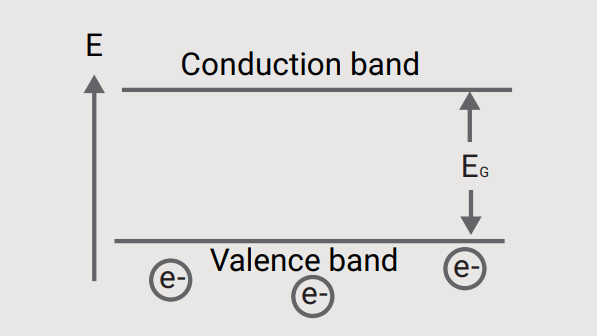
\includegraphics[width=0.6\linewidth]{figs/energy_bands.png}
    \caption{Energiebanden ~\cite{PhosphorModelingLightTools}}%
    \label{fig:energybands}
\end{figure}

Wanneer een luminescent materiaal belicht wordt zullen fotonen van het licht geabsorbeerd worden. Als de energie van de fotonen gelijk is aan het energieverschil tussen de twee banden zal een elektron van de ''valence'' naar de ''conduction'' band springen. De energie van een foton wordt bepaald door de volgende formule:

\begin{align}
E = \frac{hc}{\lambda}\label{eq:energy-foton}
\end{align}
waarbij:
\begin{align*}
h & = \text{Planck's constante} \\
c & = \text{de snelheid van het licht} \\
\lambda & = \text{de golflengte van het licht}
\end{align*}


Na een tijd zal deze elektron terug naar de ''valence'' band vallen. Dit gaat gepaart met het uitgeven van energie in de vorm van licht. In de realiteit zijn er naast deze twee banden nog andere subtoestanden die het toelaten dat een elektron kan verspringen met een lagere hoeveelheid energie. Dit bepaalt het absorptie spectrum van het materiaal.

\begin{figure}[H]
    \centering
    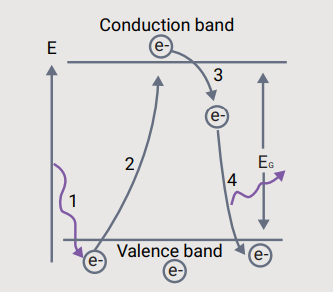
\includegraphics[width=0.6\linewidth]{figs/photolum_process.png}
    \caption{Proces luminescente materialen ~\cite{PhosphorModelingLightTools}}%
    \label{fig:photoluminescent_proc}
\end{figure}

\subsection{Witte LEDs}\label{sec:witte-leds}

Om wit licht te bekomen moeten alle drie de cones in de retina van het oog geactiveerd zijn met een gelijkaardige intensiteit. Dit komt daarnaast overeen met een centrale positie in het chromaticiteitsdiagram. Wit licht kan op een aantal verschillende manieren gegenereerd worden. Zoals eerder vermeld kan dit door kleuren te mengen. Dit kan dichromatic, trichromatic en tetrachromatic (2, 3 of 4 \gls{led}s). Op deze manieren kan een wit licht gegeneerd worden met een hoge \gls{cri} waarde. Er zijn echter veel toepassingen waar de \gls{cri} waarde niet de grootste prioriteit is.

In vele toepassingen is namelijk de efficientie van de lichtbron belangrijker. Om efficient een witte lichtbron te maken met \gls{led}s wordt gebruik gemaakt van luminescente materialen. Aan de hand van deze materialen wordt het licht van een \gls{led} met een bepaalde centrale golflengte omgezet naar licht gecentreerd rond een andere golflengte. Omdat niet al het licht geconverteerd wordt kan zo een witte lichtbron bekomen worden door bijvoorbeeld blauw licht om te zetten naar geel licht.

Naast het feit dat niet al het licht van de \gls{led} geabsorbeerd wordt zijn er ook nog verliezenn bij de omzetting van het licht. Er zijn ten eerste verliezen door de \gls{eqe} van het converterende materiaal.

\begin{align}
\eta_{\text{ext}} = \dfrac{\text{aantal fotonen uitgezonden in vrije ruimte door }\lambda\text{-converter per seconde}}{\text{aantal fotonen geabsorbeerd door }\lambda\text{-converter per seconde}}
\end{align}

Ten tweede treden er ook verliezen op door de conversie naar een hogere golflengte. Dit verschijnsel wordt ook wel de stokes shift genoemd en treed op bij het converteren van een foton met een bepaalde golflengte naar een foton met een hogere golflengte. Deze verliezen trden op omdat de energie van een foton omgekeerd evenredig is met de golflengte (\cref{eq:energy-foton}). Dit betekent dat een foton met een hogere golflengte minder energie heeft dan een foton met een lagere golflengte. Dit verschil in energie wordt omgezet in warmte.

\begin{align}
\Delta E = \frac{hc}{\lambda_1} - \frac{hc}{\lambda_2}
\end{align}

\subsection{Verschillen tussen luminescente materialen}

De verschillende luminescente materialen verschillen van elkaar in absorptie golflengtes, emissie golflengtes, eficientie, excitatie- en emissiespectra. Deze excitatie- en emissiespectra tonen aan hoeveel een luminescent materiaal elektronen naar een hoger niveau brengt en licht emiteerd bij elke golflengte. Het is dan ook logisch dat in bepaalde toepassingen een smal emissiespectrum handiger kan zijn dan een breed emissiespectrum.

\begin{figure}[H]
    \centering
    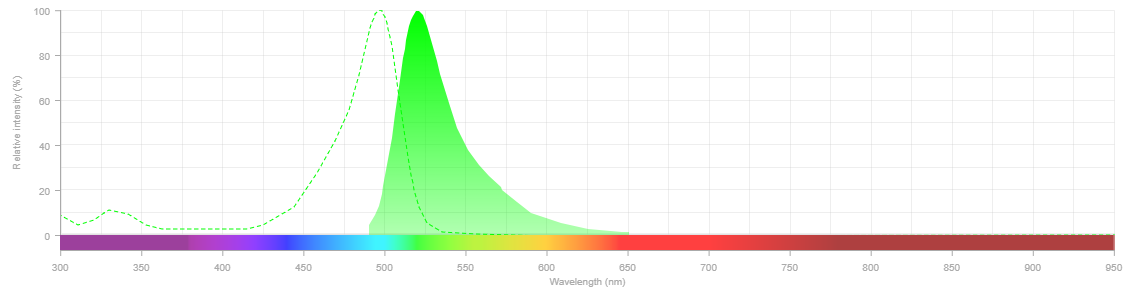
\includegraphics[width=0.9\linewidth]{spectraviewer.png}
    \caption{Emissiespectra (rhodamine 110) ~\cite{FluorescenceSpectraViewer}}%
    \label{fig:rhodamine}
\end{figure}





\chapter{Web applicatie}\label{ch:implementatie}

In dit hoofdstuk leggen we uit hoe de verschillende concepten zijn ge\"implementeerd. We beschrijven de gebruikte berekeningen, simulaties en overwegingen.

\section{Architectuur}

Er zijn veel mogelijkheden voor het maken van een app. Talen zoals Python, C++, Java, ... kunnen gebruikt worden om een app te ontwikkelen die lokaal uitgevoerd kan worden. Daarnaast kunnen ook JavaScript, HTML en CSS, met eventueel frameworks, worden ingezet om een webapp te maken.

Omdat we een zo toegankelijk mogelijke app willen bieden, hebben we besloten om een webapp te ontwikkelen. Hierdoor kan de app door iedereen gebruikt worden zonder dat er een installatie nodig is. 

% We willen echter niet dat de app onbruikbaar wordt wanneer deze niet online is, daarom moet de app ook offline beschikbaar zijn.
% % SUBJECT TO CHANGE

% Om dit te realiseren wordt op de github pagina van de app een gids voorzien om de app
% lokaal uit te voeren. Daarnaast wordt de mogelijkheid voorzien om de app ook makkelijk via de flask backend lokaal te hosten.

\subsection{Frontend}

De webapp is geschreven in Vue.js, een Javascript-framework dat werkt met componenten en reactiviteit biedt. Deze reactiviteit zorgt ervoor dat de gebruiker direct de effecten van gemaakte aanpassingen kan zien. Andere vergelijkbare opties zijn React en Angular, maar we kozen voor Vue.js omdat het de effici\"entste van de drie is voor het maken van kleine, maar toch performante apps.  

Voor de vele gebruikte standaardcomponenten (zoals knoppen, inputs, ...) maken we gebruik van het Vuetify Vue-componentframework.

We besloten om de frontend in twee talen aan te bieden: Nederlands en Engels. Dit wordt ge\"implementeerd met I18n ~\cite{krukowskiVue3I18n2023}. Via JSON-bestanden wordt voor elke taal de tekst die in de webapp gebruikt moet worden bijgehouden. De gebruiker kan eenvoudig veranderen van taal aan de hand van een knop in de app.

\subsection{Backend}

Het grootste deel van de berekeningen wordt in de webapp zelf uitgevoerd en dus op het apparaat van de client. Dit minimaliseert het aantal calls naar de server en de daarbijhorende laadtijden. We minimaliseren het aantal calls omdat we het belangrijk vinden dat de gebruiker het effect van zijn aanpassingen zo snel mogelijk ziet. Dit omdat we de gebruiker willen kunnen laten spelend leren. Als de gebruiker dan telkens vrij lang moet wachten op resultaten is dit niet mogelijk. Toch worden enkele complexere berekeningen naar de backend verplaatst. Dit komt omdat Javascript niet de meest geschikte taal is voor deze berekeningen en omdat dergelijke berekeningen het apparaat van de gebruiker te veel kunnen belasten. Toch proberen we er bij deze berekeningen ook voor te zorgen dat de tijd tot het krijgen van resultaten zo minimaal mogelijk is.

Om de complexe berekeningen uit te voeren maken we gebruik van een Python-backend met Flask. We kiezen voor Python vanwege de vele libraries voor datamanipulatie en wiskundige berekeningen, zoals numpy en scipy. Bovendien bestaat er een Python-library genaamd luxpy~\cite{smetTutorialLuxPyPython2020}, die veel berekeningen voor licht en kleur al implementeert. Deze library wordt onder andere gebruikt voor het berekenen van de \gls{cri} en Ra-waardes, het genereren van een tm30-rapport en de berekeningen voor hyperspectral image rendering.

Omdat we willen dat de reactie van de backend zo rap mogelijk is maken we gebruik van websockets. Alternatief zouden we gebruik kunnen maken van HTPP, maar dit is niet even effici\"ent. We kiezen echter voor websockets vanwege hun lagere latency.

\section{Algemene structuur}

We hebben de webapp opgedeeld in drie onderdelen. Ten eerste is er een onderdeel voor de inputs. Ten tweede is er een onderdeel voor de verschillende outputs. Ten slotte is er een onderdeel waarin de gebruiker de gebruikte modellen kan bekijken en aanpassen. We zorgen ervoor dat de inputs altijd zichtbaar zijn voor de gebruiker, omdat dit essentieel is. We willen namelijk dat de gebruiker altijd met de inputs kan spelen om te leren. Het is minder belangrijk dat alle verschillende outputs altijd zichtbaar zijn. Daarom hebben we ervoor gekozen om voor elk type output een tablad te voorzien. Daarnaast voorzien we een laatste tablad voor het databeheer. Hier kan de gebruiker de gebruikte modellen bekijken en aanpassen.

\subsection{Inputs}

In het inputgedeelte past de gebruiker verschillende componenten aan met behulp van input fields en sliders, en ziet de effecten hiervan in het outputgedeelte. De gebruiker kan kiezen uit drie standaardtypes inputs: \gls{led}s, fosforen en quantum dots. De gebruiker kan zes van deze componenten selecteren, bijvoorbeeld drie \gls{led}s, twee fosforen en \'e\'en quantum dot. We kozen ervoor zes inputs aan te bieden omdat dit voldoende speelruimte laat, maar ook realistisch blijft.

\subsection{Outputs}

De output is opgesplits in zes verschillende tabladen.

\begin{itemize}
    \item SPD
    \item Chromaticiteit
    \item Color rendering
    \item ''realistic rendering''
    \item led visualisatie
    \item databeheer
\end{itemize}

In het SPD-venster bekijkt de gebruiker de spectra van \gls{led}s via een grafiek. Daarnaast ziet de gebruiker hoe verschillende luminescente materialen deze spectra be\"invloeden. Dit venster dient als initieel inzicht in de gemaakte \gls{led}.

In het chromaticiteitsvenster bekijkt de gebruiker de chromaticiteit van de \gls{led}s en eventuele luminescente materialen. Dit biedt inzicht in de kleur van de \gls{led}s en de invloed van luminescente materialen op die kleur. Dit is cruciaal voor het leren over het ontwerpen van witte \gls{led}s. Dit venster dient voor de gebruiker als een eerste inzicht in de kleur van de gemaakte \gls{led}.

In het color-renderingvenster ziet de gebruiker de color rendering metrieken (\gls{cri} of tm30) van de \gls{led}s en luminescente materialen. Hierdoor krijgt de gebruiker een beter beeld van hoe goed de \gls{led}s kleuren kunnen weergeven, wat essentieel is voor de perceptie van de belichting. Dit venster dient dus voor de gebruiker als een inzicht in de kleurweergave van de gemaakte \gls{led}.

In het ''realistic rendering''-venster krijgt de gebruiker een realistische weergave van de verlichting in een ruimte. De app toont hierbij standaard een vergelijking met D65 (daglicht) om een beter beeld te geven van hoe de verlichting er in werkelijkheid uit zou zien. Deze vergelijking kan ook aangepast worden naar een aantal andere belangrijke lichtbronnen. Dit venster dient dus voor de gebruiker om te leren over hoe de belichting met de gemaakte \gls{led} er in werkelijkheid uit zou zien.

In het led-visualisatievenster krijgt de gebruiker een idee van hoe de chip van de gemaakte \gls{led} eruitziet. De visualisatie toont \gls{led}s als gekleurde rechthoeken, fosforen als gekleurde kristallen en quantum dots als gekleurde puntjes. In dit venster kan de gebruiker op een eenvoudige manier leren over hoe een \gls{led} chip eruit zou kunnen zien. 

In het ''data management''-venster beheert de gebruiker de data van de app. Hier bekijkt de gebruiker welke modellen worden gebruikt voor de spectra van \gls{led}s en luminescente materialen. Daarnaast kan de gebruiker eigen luminescente materialen toevoegen, het referentiespectrum voor color rendering aanpassen en het type color rendering wijzigen. Tot slot biedt de app een methode om een eigen formule te gebruiken voor de standaard spectra van luminescente materialen en het model voor de \gls{led}s.

\section{Structuur Vue}

De webapp in Vue is opgebouwd met een structuur van componenten en views. De views vormen de verschillende pagina's van de app, terwijl de componenten de herbruikbare onderdelen zijn die binnen deze views gebruikt worden. We kozen ervoor slechts gebruik te maken van \"e\"en view om de app zo eenvoudig mogelijk te houden.

Het werken met componenten biedt als voordeel dat ze herbruikbaar zijn. Zo gebruiken we bijvoorbeeld binnen het databeheer tablad meerdere dezelfde componenten voor het tonen van modellen. Daarnaast kunnen componenten worden aangepast met ''properties''. Zo kan de gebruiker bijvoorbeeld zelf inputs defini\"eren, die vervolgens in de views worden toegepast.

De webapp bestaat uit een groot aantal componenten en \'e\'en view. Omdat de app uit veel componenten bestaat, moeten we deze onderling kunnen laten communiceren. Zo moeten we bijvoorbeeld de \gls{cct} waarde die in het ene component berekend wordt versturen naar een ander component. We kunnen dit bijvoorbeeld doen aan de hand van ''events'', waarbij een component een event stuurt dat door een andere component wordt opgevangen. 

Wanneer componenten die niet direct aan elkaar gekoppeld zijn data moeten delen, kan dit complex worden. Zo zou bijvoorbeeld als een component een event moet sturen naar een ver verbonden component een keten afgelegd moeten worden. Dit betekent dat \'e\'en component een event ontvangt en dit moet doorsturen. Dit gaat zo verder tot de bestemming. Om dit te vereenvoudigen, maken we in de app gebruik van ''pinia'' stores. Deze globale structuren slaan data op en maken deze beschikbaar voor componenten, waardoor het delen van data tussen verschillende componenten eenvoudig blijft. Daarnaast kunnen we in pinia stores gebruik maken van de ''persistent'' state om caching toe te voegen. Het is echter niet altijd beter om stores te gebruiken, omdat dit de app complex kan maken. Daarnaast zijn stores ook minder efficient.


\begin{figure}[H]
    \centering
    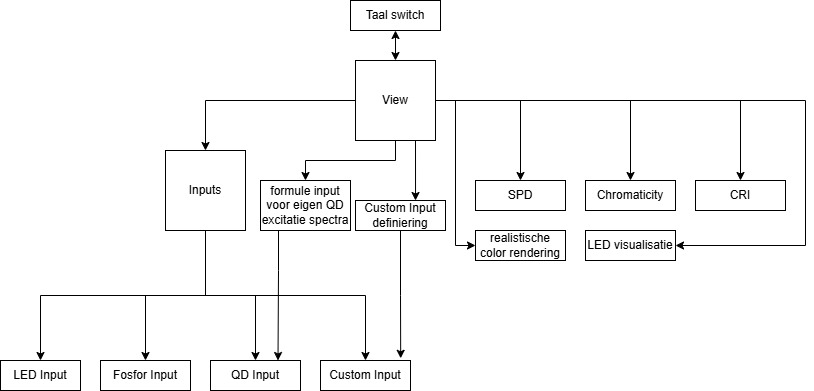
\includegraphics[width=0.9\linewidth]{structuur.jpg}
    \caption{Structuur Vue app}%
    \label{fig:vue_structure}
\end{figure}

\section{Implementatie inputs}

De inputs vormen het belangrijkste onderdeel van de app. Via deze inputs zorgen we ervoor dat de gebruiker kan experimenteren en leren van de effecten van zijn aanpassingen. De app biedt, zoals eerder vermeld, drie standaardtypes inputs: inputs voor \gls{led}s, fosforen en quantum dots.

Naast deze standaardinputs kan de gebruiker ook een input voor een luminescent materiaal maken met een csv-bestand en enkele scaling parameters. We bieden de mogelijkheid om eigen inputs te maken voor niet lerende gebruikers om te kunnen experimenteren. Zo kan bijvoorbeeld iemand die met een specifiek luminescent materiaal wil experimenteren dit doen. Deze input biedt echter wel minder flexibiliteit dan de standaardinputs, aangezien alleen de scaling parameters en de \gls{plqy}-waarde aangepast kunnen worden, dit omdat we bij deze input gebruik maken van vaste spectra en geen aanpasbare modellen.  

Voor het werken met de inputs kiest de gebruiker via een selectiemenu. Hierbij maken we gebruik van de reactiviteit van vue om enkel de geselecteerde inputs te tonen. We doen dit aan de hand van conditional rendering, waarbij alle componenten wel ingeladen zijn, maar enkel de geselecteerde effectief getoond worden.

We slaan de data van de inputs op in een van de eerder vermelde ''pinia'' stores. We maken gebruik van deze store omdat we de data van de inputs moeten gebruiken in verschillende componenten. Zo wordt bijvoorbeeld de data gebruikt om de stralingsstroom te berekenen, maar ook om de chromaticiteit te berekenen.

\subsection{LED Input}

Om een \gls{led} toe te voegen, moet de gebruiker een \gls{led} selecteren uit de beschikbare inputtypes. Vervolgens kan de gebruiker de parameters waarmee hij/zij wil experimenteren aanpassen met behulp van input fields en sliders. We kozen ervoor de fields en sliders te gebruiken omdat dit de gebruiker zowel toelaat specifieke waarden in te geven en met waarden te spelen.

We kozen ervoor om de \gls{led} input te beperken tot de belangrijkste parameters.

\begin{itemize}
    \item Centrale golflengte
    \item \gls{fwhm}
    \item Ingangsvermogen
    \item \gls{eqe}
\end{itemize}

We kozen voor deze parameters omdat deze de belangrijkste zijn voor het maken van een \gls{led}. De centrale golflengte en \gls{fwhm} bepalen de kleur van de \gls{led}, het ingangsvermogen bepaalt de lichtstroom en de \gls{eqe} bepaalt hoe effici\"ent de \gls{led} is in het omzetten van elektrische energie naar licht. Dit zijn dan ook de parameters die het belangrijkste zijn om al spelend te leren over de eigenschappen van \gls{led}s.

We kozen ervoor de \gls{eqe}-waarde onaanpasbaar te laten omdat deze waarde uit een model komt. De gebruiker kan echter wel de \gls{eqe}-waarde aanpassen door een eigen model te gebruiken (\cref{sec:eqe}).

\begin{figure}[H]
    \centering
    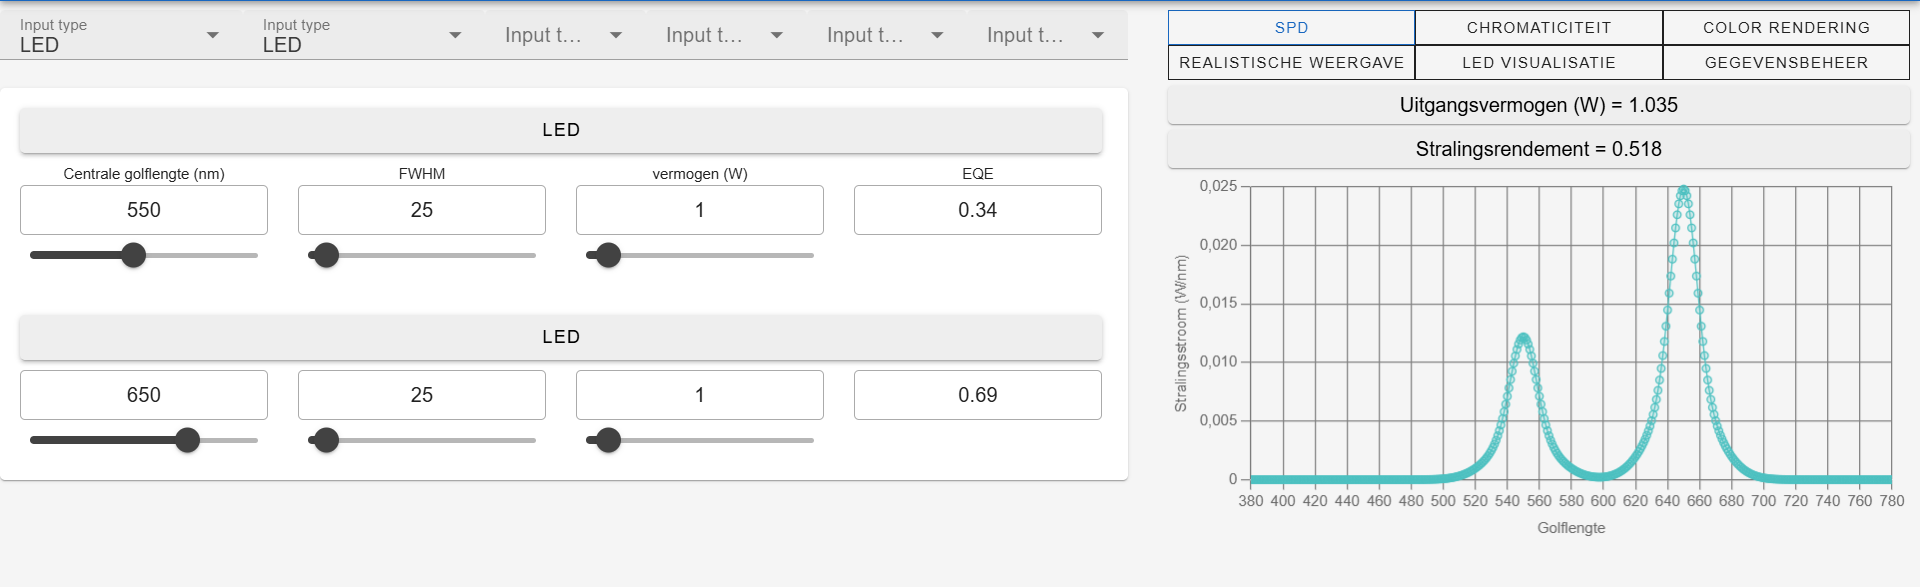
\includegraphics[width=1\linewidth]{figs/led_input.png}
    \caption{Voorbeeld \gls{led} inputs}%
    \label{fig:led_input}
\end{figure}

\subsection{Fosfor input}

Net zoals bij de \gls{led} input, moet de gebruiker voor het werken met fosforen een fosfor selecteren uit de beschikbare inputtypes. Hierbij voorzien we opnieuw input fields en sliders om de parameters specifiek en spelend aan te kunnen passen.

We kozen ervoor de volgende parameters aan de gebruiker aan te bieden.

\begin{itemize}
    \item Centrale excitatiegolflengte
    \item Centrale emissiegolflengte
    \item Excitatiebandbreedte
    \item Emissiebandbreedte
    \item concentratie
    \item \gls{plqy}
\end{itemize}

Deze parameters zijn de belangrijkste voor het maken van een fosfor. De centrale golflengtes en bandbreedtes bepalen de kleur van de fosfor, de concentratie bepaalt de hoeveelheid energie die de fosfor kan absorberen en de \gls{plqy} bepaalt hoe effici\"ent de fosfor is in het omzetten van geabsorbeerde energie naar licht. Daarnaast kan de gebruiker aan de hand van de centrale golflengtes leren over de gevolgen van de stokes shift (\cref{sec:witte-leds}).

We kozen ervoor om bij het selecteren van een fosfor de excitatiebandbreedte, emissiebandbreedte en \gls{plqy} standaardwaarden te geven.

\begin{itemize}
    \item Excitatiebandbreedte: 90 nm
    \item Emissiebandbreedte: 100 nm
    \item \gls{plqy}: 0.9
\end{itemize}

Deze waarden zijn standaardwaarden die een realistisch beeld geven van een gewoonlijk fosfor.

\begin{figure}[H]
    \centering
    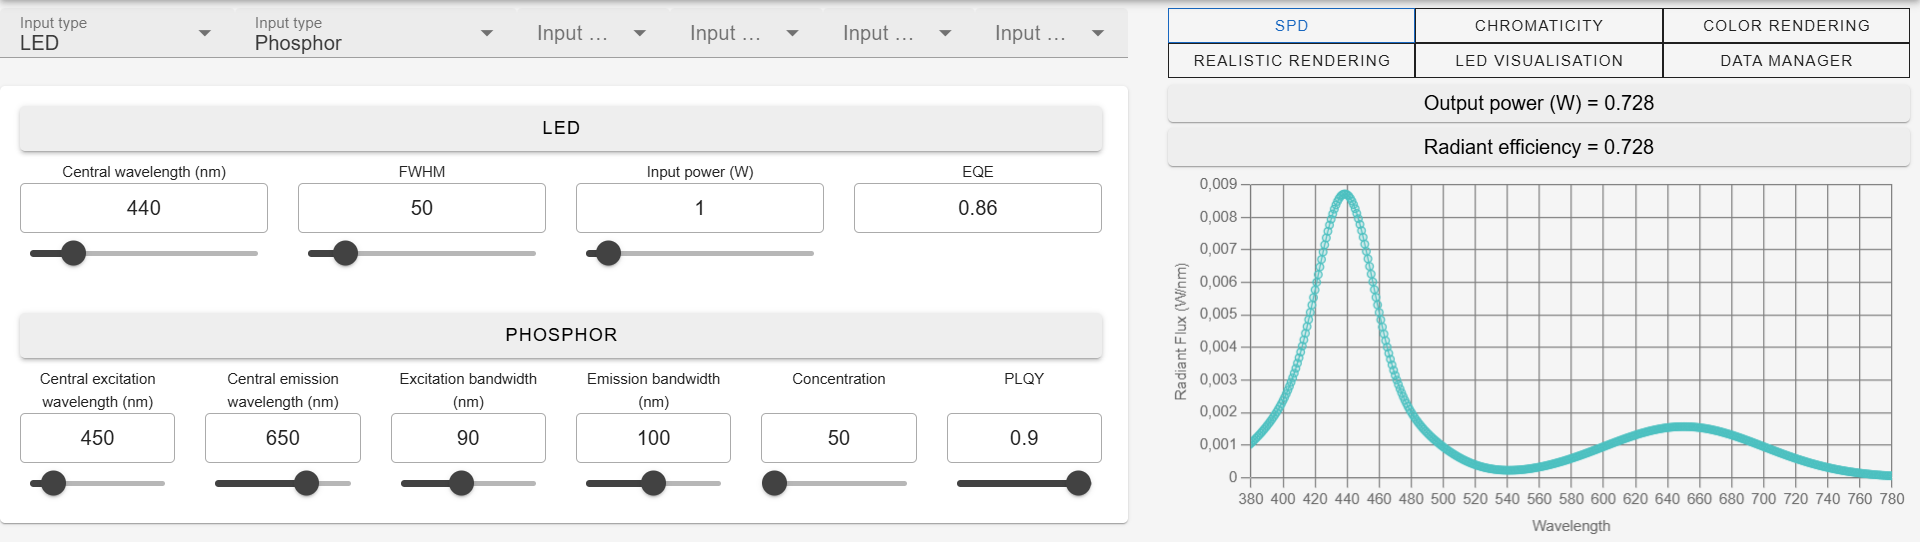
\includegraphics[width=1\linewidth]{fosfor_input.png}
    \caption{Voorbeeld fosfor inputs}%
    \label{fig:phos_input}
\end{figure}

\subsection{Quantum dot input}

De quantum dot input lijkt op de fosfor input. De gebruiker past, net zoals bij de fosfor input, de centrale emissiegolflengte, emissiebandbreedte, concentratie, en PLQY-waardes aan. De parameters voor de excitatie blijven echter onveranderd, omdat het standaardmodel voor het excitatiespectrum geen centrale excitatiegolflengte gebruikt. Wanneer echter een aangepaste formule wordt gebruikt, kan de gebruiker deze waarden wel aanpassen.

Voor de inputparameters die overeenkomen met de fosfor input gebruiken we achterliggend dezelfde variabelen. We doen dit op deze manier om zo het aantal parameters in de ''pinia'' stores zo gelimiteerd mogelijk te houden. Zo zorgen we ervoor dat de app zo effici\"ent mogelijk blijft.

Net zoals bij de fosfor input, voorzien we standaardwaarden voor de emissiebandbreedte en \gls{plqy}.

\begin{itemize}
    \item Emissiebandbreedte: 40 nm
    \item \gls{plqy}: 0.8
\end{itemize}

\begin{figure}[H]
    \centering
    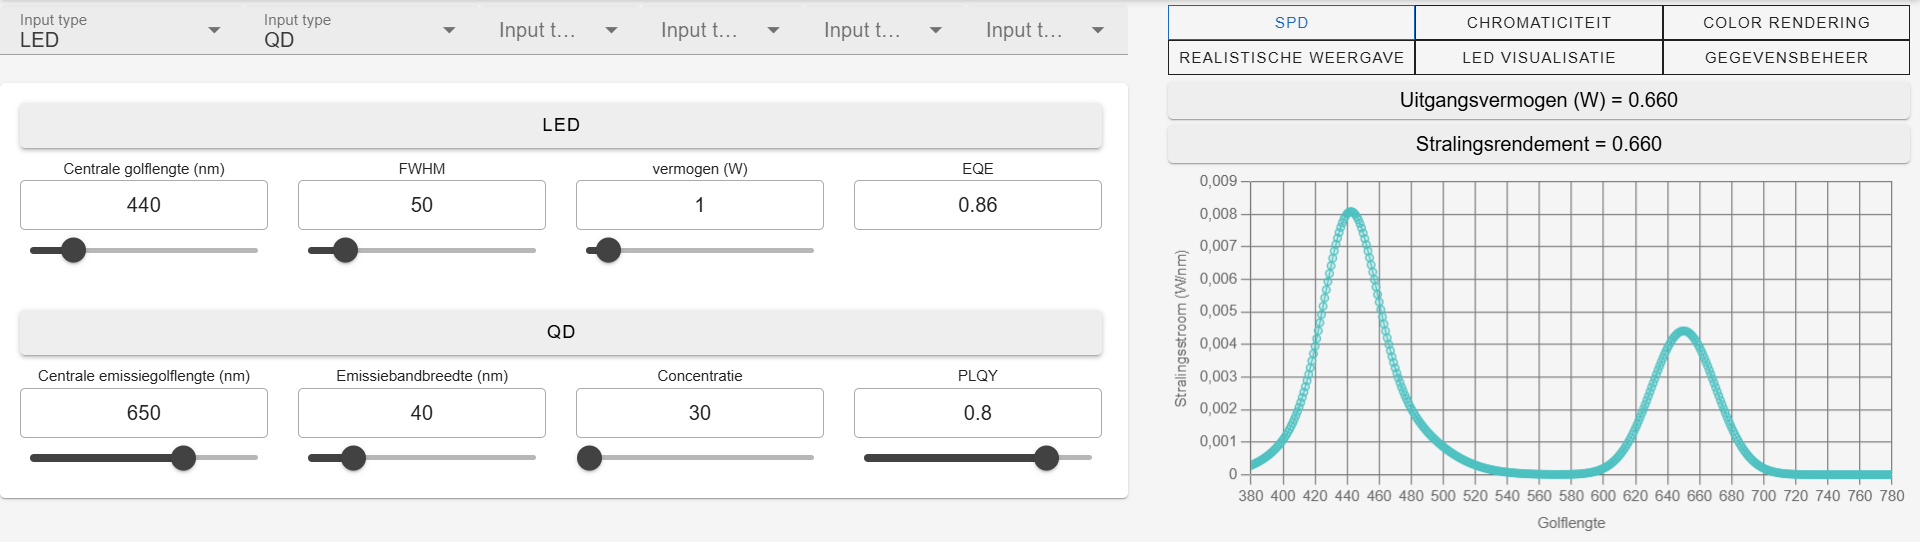
\includegraphics[width=1\linewidth]{QD_input.png}
    \caption{Voorbeeld quantum dot inputs}%
    \label{fig:QD_input}
\end{figure}

\subsection{Luminescent materiaal input}\label{sec:luminescent_input}

De gebruiker kan naast de standaard luminescente materialen ook eigen luminescente materialen toevoegen. Dit doet hij door een \gls{csv}-bestand te uploaden met de kolommen ''Wavelength'', ''Excitation'' en ''Emission''.  

Daarnaast stelt de gebruiker een initi\"ele schalingsfactor in en geeft hij een naam aan het materiaal. De schalingsfactor zorgt ervoor dat de geabsorbeerde en ge\"emitteerde energie logisch samenwerkt met de concentratieschalingsfactor.  


\begin{figure}[H]
    \centering
    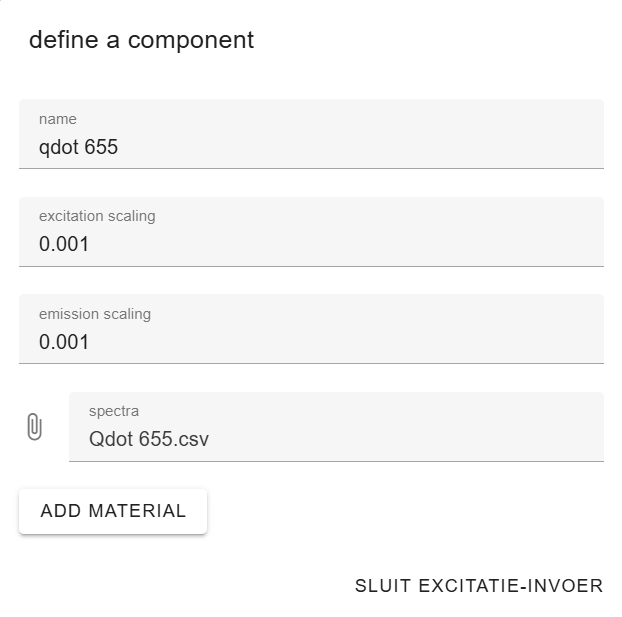
\includegraphics[width=0.5\linewidth]{custom_input_definition.png}
    \caption{Voorbeeld upload luminescent materiaal}%
    \label{fig:luminescent_input_definition}    
\end{figure}

De naam van het materiaal wordt gebruikt om alle nodige informatie van het materiaal op te slaan in een store voor de toegevoegde materialen. De data wordt opgeslagen in een object waarbij de keys de naam van het materiaal zijn en de values een object bevatten voor de excitatie- en emissiespectra. Daarnaast worden ook schalingswaarden opgeslagen. Deze schalingswaarden worden voorzien omdat we niet kunnen voorspellen hoe de waarden van de gebruiker zullen zijn. De schalingswaarden zorgen ervoor dat de gebruiker de data kan aanpassen zodat realistische waarden bekomen worden in de simulaties.

We kunnen de gebruiker van deze inputs een stuk minder laten aanpassen omdat bepaalde zaken zoals de golflengtes inherent zijn aan het materiaal. We laten de gebruiker wel nog toe om de volgende parameters aan te passen.

\begin{itemize}
    \item Schalingsfactoren
    \item concentratie
    \item \gls{plqy}
\end{itemize}

Omdat deze elementen ook geselecteerd moeten kunnen worden, hebben we componenten gemaakt die op basis van de geselecteerde waarde informatie ophalen uit de store en tonen aan de gebruiker. Hierbij moeten we rekening houden met de mogelijkheid dat de gebruiker een materiaal selecteert dat niet bestaat. In dat geval mag het component niet getoond worden. Dit kan eenvoudig gecontroleerd worden door te verifi\"eren of de naam behoort tot de beschikbare items en niet gelijk is aan LED, fosfor of QD.

\begin{figure}[H]
    \centering
    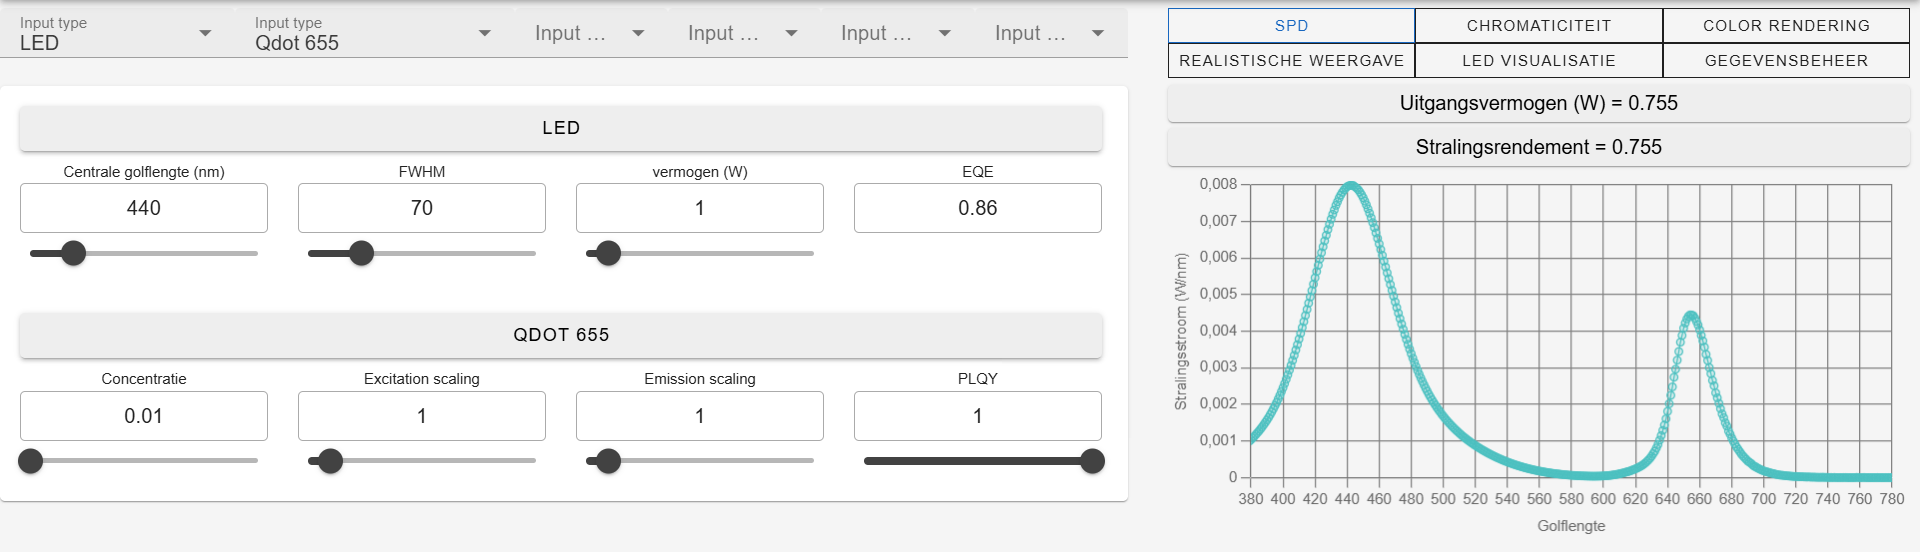
\includegraphics[width=1\linewidth]{qdot655_input.png}
    \caption{Voorbeeld luminescent materiaal input}%
    \label{fig:luminescent_input}
\end{figure}

\section{Implementatie LEDs en SPD}

\subsection{Implementatie LED model}

Het belangrijkste onderdeeel van de app dat we implementeerden, is het model van de \gls{led} en de omzetting ervan naar de \gls{spd}. We starten met een model of spectrum dat het relatieve vermogen per golflengte weergeeft. Op basis hiervan zetten we dit om naar de \gls{spd} van de \gls{led}.

Oorspronkelijk gebruikten we een gaussiaans model met het centrum op de centrale golflengte van de \gls{led} en een breedte bepaald door het \gls{fwhm}. Er zijn echter meerdere manieren om een \gls{led} te modelleren. Zo zouden we bijvoorbeeld ook een lorentziaans model kunnen gebruiken. Beide van deze modellen zijn echter relatief eenvoudig en geven geen volledig accuraat beeld van een \gls{led}. 

Om de simulaties accurater te maken, schakelden we over naar een wiskundig model dat specifiek ontwikkeld werd voor multichip \gls{led}s~\cite{ohnoSpectralDesignConsiderations2005}. Dit model wordt, net als het gaussiaanse model, bepaald door de centrale golflengte en het \gls{fwhm} van de \gls{led}. Het model bepaald de \gls{spd} van de \gls{led} aan de hand van de volgende formule:

\begin{equation}
    S_{\text{LED}}(\lambda, \lambda_0, \Delta \lambda_{0.5}) = \frac{\displaystyle g(\lambda, \lambda_0, \Delta \lambda_{0.5}) + 2g^5(\lambda, \lambda_0, \Delta \lambda_{0.5})}{3},
\end{equation}

waarin g gelijk is aan

\begin{equation}
    g(\lambda, \lambda_0, \Delta \lambda_{0.5}) = \exp\left(-\left[\frac{\lambda - \lambda_0}{\Delta \lambda_{0.5}}\right]^2\right).
\end{equation}

met symbolen:
\begin{itemize}
    \item \(\lambda\): De golflengte parameter (nm).
    \item \(\lambda_0\): De central golflengte van de \gls{led} emissie, dus de golflengte waarop het relatief vermogen het hoogste is.
    \item \(\Delta \lambda_{0.5}\): De \gls{fwhm}, stelt de spectrale breedte van de \gls{led} voor.
\end{itemize}

Omdat dit model een relatief model is, waarbij de hoogste waarde 1 is en de laagste 0, passen we een normalisatie toe om verdere berekeningen correct te laten verlopen. We normaliseren eenvoudigweg door de som van alle datapunten als normalisatiefactor te gebruiken. Door vervolgens elk datapunt door deze factor te delen, bekomen we een model met een totaal standaard vermogen van \'e\'en Watt. Omdat deze factor verschilt afhankelijk van de ingestelde parameters moeten we dit telkens opnieuw berekenen. Dit zorgt voor een lichte vertraging, we kiezen ervoor toch dit model te belijven gebruiken omdat de verhoogde accuraatheid belangrijker is dan de kleine vertraging. Dankzij deze aanpassing kunnen we het vermogen van een \gls{led} eenvoudig instellen door te vermenigvuldigen met het ingestelde vermogen. Daarnaast kunnen we de \gls{eqe} op dezelfde manier direct vermenigvuldigen.

\begin{figure}[H]
    \centering
    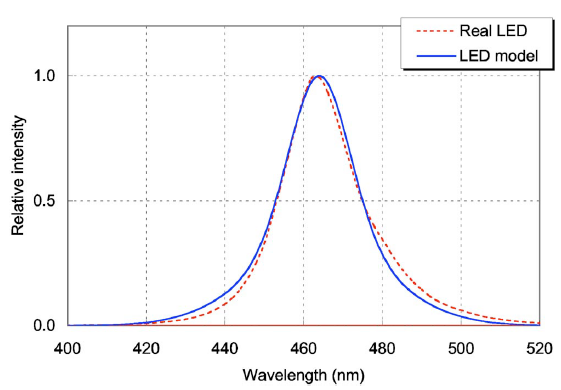
\includegraphics[width=0.8\linewidth]{figs/ohno.png}
    \caption{Multichip led model (Ohno)~\cite{ohnoSpectralDesignConsiderations2005}}%
    \label{fig:OhnoModel}
\end{figure}

\subsection{Implementatie SPD} % TO BE REWRITTEN

De overgang van een \gls{led}-model naar de \gls{spd} is vrij eenvoudig. Ten eerste maken we voor elke aanwezige \gls{led} de overgang van een relatief vermogen naar een effectief vermogen per nanometer. Door de eerder toegepaste normalisatie kunnen we dit doen door het relatieve vermogen van het model te vermenigvuldigen met het door de gebruiker ingestelde vermogen. Ten slotte vermenigvuldigen we ook de \gls{eqe} van de \gls{led}. Door deze vermenigvuldigingen krijgen we een realistische simulatie van de \gls{spd} van een \gls{led}. Wanneer een gebruiker meerdere \gls{led}s toevoegt, tellen we eenvoudigweg de verschillende bekomen \gls{spd}-waarden op om de totale \gls{spd} te verkrijgen.

Vervolgens tonen we het bekomen \gls{spd}-model aan de gebruiker in een grafiek. Hierin tonen we de stralingsstroom tussen 380 en 780 nm (het zichtbare spectrum). Naast deze grafiek geven we ook het uitgaande vermogen en de ''radiant efficiency'' (uitgaand vermogen / ingaand vermogen) weer. Dit helpt de gebruiker te begrijpen welke effecten verschillende technieken hebben op het genereren van witte \gls{led}s. Zo kan de gebruiker bijvoorbeeld zien waarom het combineren van rode, groene en blauwe \gls{led}s niet noodzakelijk even effici\"ent is als een blauwe \gls{led} met een gele fosfor.

Met deze grafiek kan de gebruiker zich al een eerste idee vormen over de eigenschappen van de gemaakte \gls{led}. Dit gebeurt aan de hand van de golflengtes van de pieken, de breedte van de pieken en de relatieve intensiteit van de pieken.

\subsection{Model EQE}\label{sec:eqe}

Omdat de berekening van de \gls{spd} gebruik maakt van de \gls{eqe} van een \gls{led}, is er ook een model voor nodig. Een realistisch model van \gls{eqe} is vooral belangrijk vanwege de ''green gap''. Dit is een kloof in de \gls{eqe}-waarden van \gls{led}s, die zich vooral bevindt bij de golflengtes die geassocieerd worden met groene \gls{led}s. Dit verklaart waarom het maken van witte \gls{led}s door simpelweg \gls{led}s te combineren momenteel ineffici\"ent is. Het \gls{eqe}-model leiden we af uit meetresultaten van \gls{led}s uit 2017 en 2018~\cite{hahnClosingGreenGapb}.  

Omdat het echter niet zeker is dat deze ''green gap'' blijft bestaan of even ernstig blijft, bieden we de gebruiker de mogelijkheid om een \gls{csv}-bestand met \gls{eqe}-waarden te uploaden. Dit bestand hoeft niet per se realistische waarden te bevatten. Zo kan het bijvoorbeeld ook worden gebruikt om te experimenteren met scenario's waarin de ''green gap'' niet bestaat of niet langer een groot probleem is. Dit maakt de app direct flexibeler en beter bestand tegen mogelijke veranderingen in de toekomst. Daarnaast laten we zo ook lerende gebruikers toe om te experimenteren met verschillende scenario's. Hierdoor kunnen ze beter begrijpen waarom de ''green gap'' een probleem is en hoe dit kan worden opgelost.

\begin{figure}[H]
    \centering
    \resizebox{0.7\textwidth}{!}{% This file was created with tikzplotlib v0.10.1.
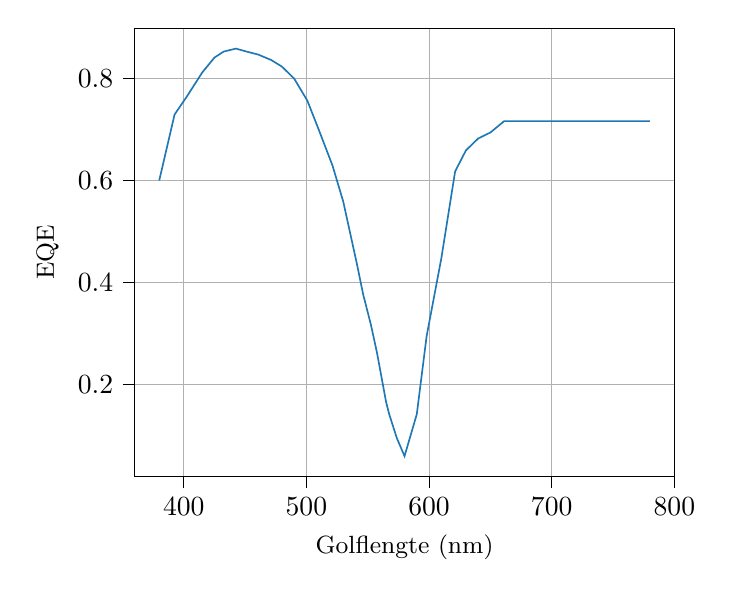
\begin{tikzpicture}

\definecolor{darkgray176}{RGB}{176,176,176}
\definecolor{steelblue31119180}{RGB}{31,119,180}

\begin{axis}[
tick align=outside,
tick pos=left,
x grid style={darkgray176},
xlabel={Golflengte (nm)},
xmajorgrids,
xmin=360, xmax=800,
xtick style={color=black},
y grid style={darkgray176},
ylabel={EQE},
ymajorgrids,
ymin=0.0188235315, ymax=0.8988234985,
ytick style={color=black}
]
\addplot [semithick, steelblue31119180]
table {%
380 0.6
392.5 0.7294
402.5 0.7647
415 0.81176
425 0.8411765
432.5 0.8529412
442.5 0.8588235
451.25 0.8529412
460.75 0.8470588
471.25 0.8364706
480 0.8235294
490 0.8
500.75 0.756706
510 0.7
521.25 0.6294118
530 0.5588235
541.25 0.4352941
546.25 0.3764706
552.5 0.3176471
557.5 0.2623529
565 0.1647059
567.5 0.1411765
573.75 0.09411765
580 0.05882353
590 0.1411765
598 0.2941176
610 0.4470588
621.25 0.6176471
630 0.6588235
640 0.6823529
650 0.6941176
661.25 0.716471
670 0.716471
780 0.716471
};
\end{axis}

\end{tikzpicture}
}
    \caption{Model \gls{eqe} ~\cite{hahnClosingGreenGapb}}
    \label{fig:eqe}
\end{figure}

\section{Implementatie chromaticiteit}

Voor het implementeren van de chromaticiteit maken we gebruik van de in \cref{sec:chromaticiteit} beschreven formules. Er moet echter een kleine aanpassing worden gemaakt. We moeten namelijk overgaan van integralen naar sommen. Dit omdat de \gls{spd} van een \gls{led} een discrete functie is (\'e\'en punt per nm). De chromaticiteit kan dan berekend worden aan de hand van de volgende formules voor de tristimuluswaarden:

\begin{align}
    X &= 683.\sum_{\lambda} \bar{x}(\lambda) S(\lambda) \Delta \lambda \\
    Y &= 683.\sum_{\lambda} \bar{y}(\lambda) S(\lambda) \Delta \lambda \\
    Z &= 683.\sum_{\lambda} \bar{z}(\lambda) S(\lambda) \Delta \lambda
\end{align}

waarin:

\begin{itemize}
    \item \(\bar{x}(\lambda)\), \(\bar{y}(\lambda)\) en \(\bar{z}(\lambda)\): de color matching functies.
    \item \(S(\lambda)\): de \gls{spd} van de \gls{led}.
    \item \(\Delta \lambda\): 1 nm.
\end{itemize}

De chromaticiteit kan dan berekend worden aan de hand van de volgende formules:

\begin{align}
    x &= \frac{X}{X + Y + Z} \\
    y &= \frac{Y}{X + Y + Z} \\
    z &= \frac{Z}{X + Y + Z}
\end{align}

Voor de berekening van de chromaticiteit maken we gebruik van de color matching functies. Om deze te gebruiken, laden we een \gls{csv}-bestand in met de waarden van de color matching functies (CIE 1931 2\textdegree observer). Deze waarden worden vervolgens gebruikt om de chromaticiteit te berekenen.

Om het berekende (x, y)-punt op het chromaticiteitsdiagram te tonen, gebruiken we een canvas-element (HTML element voor tekenen) met een foto van een standaard chromaticiteitsdiagram. We tekenen het punt op dit diagram door de (x, y)-co\"ordinaten te transformeren. Daarnaast voegen we de \gls{cct}-waarde toe, omdat het moeilijk voor de gebruiker is om deze waarde direct af te lezen van het diagram.

\begin{figure}[H]
    \centering
    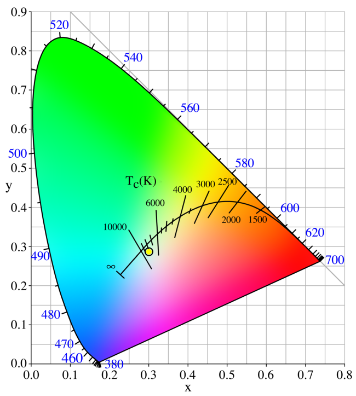
\includegraphics[width=0.5\linewidth]{figs/chromaticiteit_getekend.png}
    \caption{Voorbeeld resultaat chromaticiteit}%
    \label{fig:chromaticity_result}
\end{figure}

Het doel van de chromaticiteit is om de gebruiker een eerste idee te geven van de kleur van zijn gemaakte \gls{led}. Dit kan bijvoorbeeld de gebruiker helpen om een witte \gls{led} te maken. Daarnaast leert het de gebruiker ook dat chromaticiteit geen volledige beschrijving is van de kleur van een lichtbron. Zo kan een \gls{led} met dezelfde chromaticiteit toch een andere ervaring hebben voor een toeschouwer.

Naast de chromaticiteit worden ook de totale lichtstroom, het visueel rendement (totale lichtstroom / uitgaand vermogen) en de specifieke lichtstroom (totale lichtstroom / ingaand vermogen) getoond. De totale lichtstroom geeft de gebruiker een idee van het licht dat de \gls{led} uitstraalt. Het visueel rendement geeft de gebruiker inzicht in hoe effici\"ent de \gls{led} is in het omzetten van elektrische energie naar licht. De specifieke lichtstroom geeft de gebruiker een idee van hoeveel licht er wordt uitgestraald per watt elektrische energie. Deze waarden zijn belangrijk voor de gebruiker en kunnen bijvoorbeeld bepalend zijn bij het kiezen van een bepaalde manier om een kleur te verkrijgen (meerdere \gls{led} of luminescente materialen). Door ze hier toe te voegen krijgt de gebruiker dus een beter beeld van de eigenschappen van de gemaakte \gls{led}. Zo kan hij/zij bijvoorbeeld een \gls{led} maken met een bepaalde chromaticiteit, maar met een laag visueel rendement. Hierna kan dan bijvoorbeeld een \gls{led} bekomen worden met dezelfde chromaticiteit, maar met een hoger visueel rendement. Hierdoor leert de gebruiker over de voor en nadelen van de verschillende methoden om een kleur te bekomen.

\section{Implementatie color rendering}

\subsection{CIE Ra-15}

Het berekenen van de \gls{cri} en Ra-waarden is dankzij de Luxpy-bibliotheek zeer eenvoudig ~\cite{smetTutorialLuxPyPython2020}. De gebruiker hoeft enkel een \gls{spd} mee te geven, waarna de R0-R9-waarden berekend kunnen worden. Luxpy berekent automatisch het referentiespectrum, maar omdat we dit ook aan de gebruiker willen tonen, zodat deze kan proberen een (volgens \gls{cri}) zo goed mogelijke lichtbron te verkrijgen, hebben we de Luxpy-functie licht aangepast. Het referentiespectrum wordt door deze aaanpassing teruggegeven na een request aan de server. De \gls{cri}- en Ra-waarden worden vervolgens berekend en getoond aan de gebruiker in een staafdiagram.

We tonen de gebruiker de R0-R9-waarden, de \gls{cri}-waarde, het referentiespectrum en het eigen gemaakte spectrum. Aan de hand van de R-waarden kan de gebruiker zien welke kleuren goed worden weergegeven en welke niet. De \gls{cri}-waarde geeft de gebruiker een idee van hoe goed de kleuren over het algemeen worden weergegeven. Het referentiespectrum toont de gebruiker hoe een perfecte lichtbron eruitziet (volgens CIE Ra-15). We tonen al deze waarden zodat de gebruiker kan leren over de effecten van verschillende lichtbronnen op de kleurweergave.

Het is belangrijk dat de gebruiker leert hoe hij een lichtbron kan maken die volgens de \gls{cri}-waarde zo goed mogelijk is. Het is echter cruciaal dat de gebruiker begrijpt dat een hoge waarde niet noodzakelijk betekent dat de lichtbron effectief goed is. Zo kan bijvoorbeeld een score boven de 80 behaald worden, terwijl de waarde van R9 slechts rond de 20 ligt. Volgens \gls{cri} is dit een goede lichtbron, maar voor de mens is de R9-waarde erg belangrijk. In dit geval is de lichtbron waarschijnlijk niet ideaal. Hiervoor worden naast CIE Ra-15 ook andere methoden zoals IES TM-30 en ''realistic color rendering'' aangeboden.

\subsection{ies-tm30}

Naast CIE Ra-15 biedt Luxpy ~\cite{smetTutorialLuxPyPython2020} ook de mogelijkheid om IES TM-30-berekeningen uit te voeren en rapporten te genereren. Omdat dit een recentere en offici\"ele color rendering maat is, kozen we ervoor de gebruiker de mogelijkheid te geven om IES TM-30 te gebruiken in plaats van CIE Ra-15. Daarnaast is het ook een goede manier om te leren over de verschillen tussen verschillende maten voor kleurweergave. Een meer geavanceerde gebruiker kan dan weer kiezen welke color rendering methode het beste past bij zijn of haar toepassing. Net als bij CIE Ra-15 kunnen de benodigde berekeningen uitgevoerd worden met Luxpy.

We kozen ervoor om een eenvoudig TM-30-verslag te gebruiken met Rf, Rg, CCT en D(u,v), omdat dit de belangrijkste waarden binnen de TM-30 methode zijn. Daarnaast tonen we een gamutcirkel met daarop hue shift vectoren. Aan de hand van deze waarden kan een lerende gebruiker leren over het belang van de verschillende metrieken. Een geavanceerde gebruiker kan zich een idee vormen over de geschiktheid van zijn gemaakte lichtbron voor een bepaalde toepassing.

\section{Implementatie luminescente materialen}

Om de invloed van luminescente materialen te begrijpen, hebben we een berekening nodig die van de excitatie- en absorptiespectra naar de geabsorbeerde en ge\"emitteerde energie leidt. Zoals eerder vermeld, zijn er geen applicaties die dit reeds hebben gedaan. Bovendien zijn er geen formules beschikbaar die dit op een eenvoudige en algemene manier kunnen berekenen. Daarom besloten we zelf een formule te ontwikkelen.

\subsection{Simpele berekening}

oorspronkelijk maakten we gebruik van een simpele berekening die ook in de KU Leuven Excel werd gebruikt. Deze werkt echter alleen volledig correct voor fosforen. Daarnaast is deze niet volledig theoretisch onderbouwd, maar volgt deze de verwachte effecten van fosforen (zoals de Stokes shift). De geabsorbeerde energie wordt in deze methode berekend aan de hand van een exponentieel verval.

\begin{equation} E_{abs} = \text{S} . (1 - \exp(-\text{C}.3.\sqrt{2.\pi}.\text{norm}(\lambda,\lambda_{ex},\text{excitatiebreedte/2}) )) \end{equation} waarbij C de concentratie is en S de stralingsstroom.\

Omdat deze formule gebaseerd is op het gebruik van de normale verdeling binnen het exponenti\"ele verval, is deze alleen correct voor fosforen. Voor quantum dots en andere materialen waarbij de excitatiespectra geen normale verdeling volgen, is deze formule minder geschikt.

Om het ge\"emitteerde vermogen te berekenen, maken we gebruik van een simpele formule waarin we rekening houden met de verschillen in concentraties tussen de verschillende aanwezige materialen en de Stokes shift.

\begin{equation} E_{em} = E_{abs} . QE . \text{emissiespectrum} . C . (1 - (\lambda_{em}-\lambda_{ex}/\lambda_{ex})) \end{equation} waarbij C het percentage van alle luminescente materialen is dat deze inneemt.

%figure
\begin{figure}[H]
    \centering
    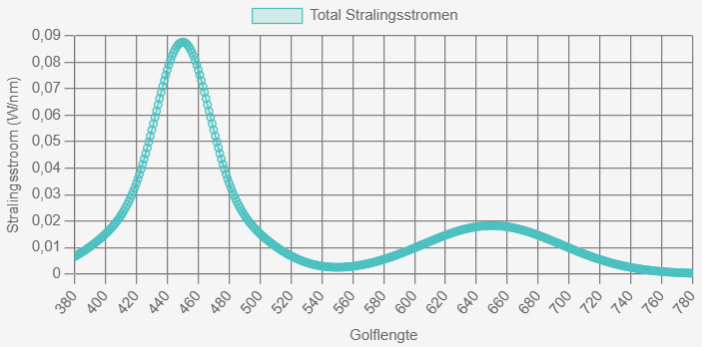
\includegraphics[width=0.45\linewidth]{figs/spectrum_fosfor_simple.png}
    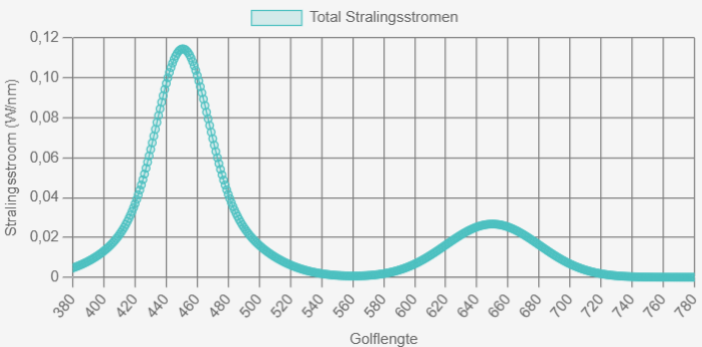
\includegraphics[width=0.45\linewidth]{spectrum_QD_simple.png}
    \caption{Voorbeeld resultaten met simpel model (links = fosfor, rechts = quantum dot)}%
    \label{fig:result_simple}
\end{figure}

\subsection{Geavanceerde berekening}\label{sec:advanced}

Om een correctere berekening te maken zodat een lerende gebruiker de effecten van luminescente materialen correct kan leren kennen ontwikkelden we een geavanceerd model. We ontwikkelden dit geavanceerd model op een meer theorethische manier zodat alle effecten van de luminescente materialen correct gemodeleerd zijn.
Deze formule baseren we op de verdeling van fotonen en de verdeling van energie.
Daarnaast maken we gebruik van de relaties tussen excitatie- en emissiespectra en de
geabsorbeerde en ge\"emiteerde energie.
Deze formule kan gebruikt worden voor elk luminescent materiaal waarvan de
excitatie- en emissiespectra gekend zijn en is dus meer geschikt voor de toepassing dan de simpele formule.

We weten dat 

\begin{equation}
    f_1(\lambda) = \text{De distributie van geabsorbeerde energie en}
\end{equation}
\begin{equation}
    f_2(\lambda) = \text{De distributie van ge\"emiteerde energie}.
\end{equation}

Hierbij weten we dat 

\begin{equation}
    f_1(\lambda) = f'_1(\lambda) . SPD(\lambda)
\end{equation}
met $f'_1(\lambda)$ het excitatiespectrum van het gebruikte luminescente materiaal.

Nu moet echter nog $f_2(\lambda)$ berekend worden. We weten dat de distributie van het aantal fotonen evenredig is met

\begin{equation}
    f(\lambda).\lambda = g(\lambda) \text{ (de verdeling van de fotonen)} \label{eq:distFot}
\end{equation}
want
\begin{equation}
    E(\lambda) \sim 1/\lambda \text{ (de energie van een foton)}
\end{equation}

Als we veronderstellen dat \gls{plqy} = 100\% (het aantal geabsorbeerde fotonen/het aantal ge\"emiteerde fotonen van een materiaal). Dan weten we dat het aantal fotonen gelijk blijft en kunnen we stellen dat

\begin{equation}
    \int g_1(\lambda) \, d\lambda = \int g_2(\lambda) \, d\lambda
\end{equation}
Met $g(\lambda)$ de verdeling van de fotonen.

uit \ref{eq:distFot} volgt dan dat

\begin{equation}
    \int f_1(\lambda).\lambda \, d\lambda = \int f_2(\lambda).\lambda \, d\lambda
\end{equation}
Met 

Omdat $f_1(\lambda)$ gekend is en we de vorm van $f_2(\lambda)$ kennen. Deze heeft namelijk dezelfde vorm als het emissiespectrum $f'_2(\lambda)$. We kennen dus $f_2(\lambda)$ op een schalingsfactor na dus

\begin{equation}
    f_2(\lambda) = a.f'_2(\lambda)
\end{equation}
Met $f'_2(\lambda)$ het emissiespectrum van het luminescente materiaal en a de schalingsfactor.

Dan kunnen we a op de volgende manier vinden

\begin{equation}
    \int f_1(\lambda).\lambda \, d\lambda = \int a.f'_2(\lambda).\lambda \, d\lambda
\end{equation}

\begin{equation}
    \Leftrightarrow
    a = \int f_1(\lambda).\lambda \, d\lambda / \int f'_2(\lambda).\lambda \, d\lambda
\end{equation}

Tot nu toe hebben we verondersteld dat \gls{plqy} gelijk is aan 100\%. Dit zal echter meestal niet het geval zijn. Om hier rekening mee te houden vermenigvuldigen we op het einde nog met \gls{plqy} en is dus

\begin{equation}
    f_2(\lambda) = a.PLQY.f'_2(\lambda)
\end{equation}

\begin{figure}[H]
    \centering
    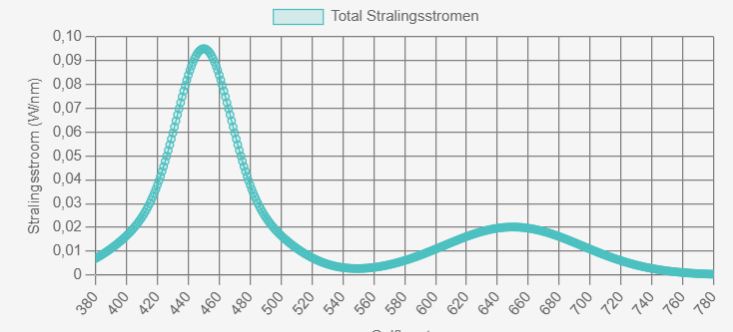
\includegraphics[width=0.45\linewidth]{spectrum_fosfor_advanced.png}
    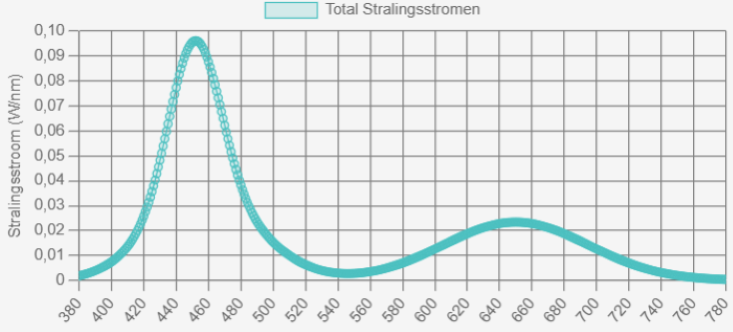
\includegraphics[width=0.45\linewidth]{spectrum_QD_advanced.png}
    \caption{Voorbeeld resultaten met geavanceerd model (links = fosfor, rechts = quantum dot)}%
    \label{fig:result_advancded}
\end{figure}

Zoals te zien is in \ref{fig:result_simple} en \ref{fig:result_advancded} 
zijn de resultaten bij het gebruik van fosforen inderdaad zeer vergelijkbaar.
Bij quantum dots is er echter een groot verschil. 
Dit omdat nu correct rekening gehouden wordt met de niet normale verdeling van
het excitatiespectrum.

\subsection{Spectra}

We maken gebruik van een algemeen model van de spectra zodat we de gebruiker kunnen laten zien wat de effecten zijn van de verschillende
parameters van luminescente materialen. Hiervoor moeten we dus per standaard materiaal een model gemaakt worden.

Voor fosforen maakten we een model dat een normale verdeling volgt. Dit omdat de meeste
fosforen een excitatie- en emissiespectrum hebben die ongeveer een normale verdeling volgen. Deze
zijn meestal beiden gecentreerd rond de excitatie- en emissiegolflengte met een bepaalde
''skew''. Het is dan ook voor deze reden dat we de mogelijkheid voorzien om het model aan te passen naar bijvoorbeeld een normaalverdeling met ''skew'' (\cref{sec:data_manager}).

\begin{figure}[H]
    \centering
    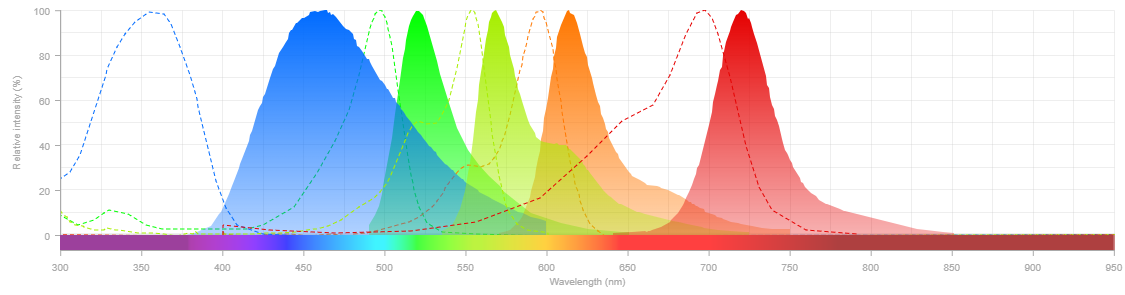
\includegraphics[width=0.9\linewidth]{spectraviewer_normPhos.png}
    \caption{Voorbeeld fosfor spectra (stippellijn = excitatie, vol = emissie) ~\cite{FluorescenceSpectraViewer}}%
    \label{fig:spectra_fosfor}
\end{figure}

Het modeleren van quantum dots is echter moeilijker. Ze hebben net zoals
fosforen een normaal verdeeld emissiespectrum. Het excitatiespectrum is echter
niet normaal verdeeld. Ze volgen eerder een dalende lijn.

\begin{figure}[H]
    \centering
    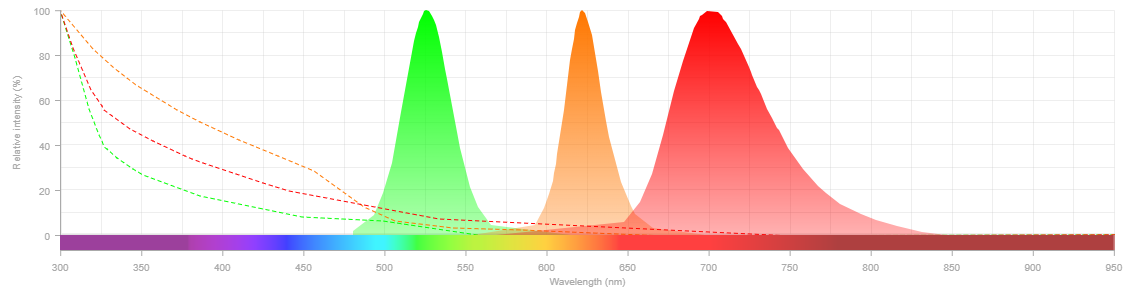
\includegraphics[width=0.9\linewidth]{spectraviewer_QD.png}
    \caption{Voorbeeld fosfor QD (stippellijn = excitatie, vol = emissie) ~\cite{FluorescenceSpectraViewer}}%
    \label{fig:spectra_QD}
\end{figure}

Daarnaast zijn er ook in de lijn soms pieken te zien. Ten laatste varieert de lijn ook sterk afhankelijk van de configuratie van de quantum dot. Dit maakt het modelleren van quantum dots moeilijker dan fosforen. Zo bestaan er wel modellen voor quantum dots maar
zijn deze vaak zeer specifiek afhankelijk van de configuratie van de quantum dot. Dit zijn dan bijvoorbeeld modellen die een empirische fit zijn van meetresultaten.

Omdat we een zo algemeen mogelijk model willen maken voor het excitatiespectrum is dit type model dus geen goede optie. Ook zou het aanpassen van dit type
model weinig bruikbaar zijn omdat het meestal gebruik maakt van moeilijkere parameters. Die ook weinig relevant zijn voor de gebruiker van onze app.

Uit deze vaststellingen besloten we om een simpel model te gebruiken voor het excitatiespectrum
van de quantum dots. Dit model volgt een dalende exponentiele lijn. Dit model is echter niet
perfect en dus voorzien we de optie om de gebruikte formule aan te passen. Daarnaast voorzien we hiervoor ook de mogelijkheid om eigen luminescente materialen toe te voegen. Dit bijvoorbeeld met gemeten data van een specifieke quantum dot voor volledige accuraatheid.

\begin{equation}
    0.03 . \exp\left(\frac{\log(0.1) . (\lambda - 360)}{\lambda_{em} - 360}\right)
\end{equation}

\begin{figure}[H]
    \centering
    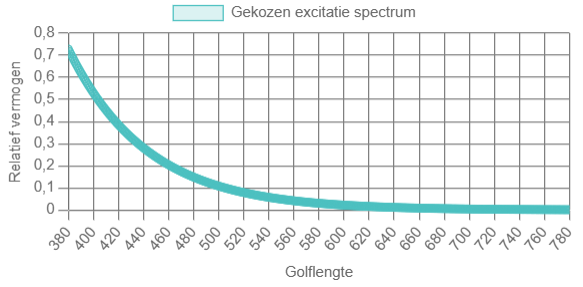
\includegraphics[width=0.9\linewidth]{excitatie_QD.png}
    \caption{Standaard excitatiespectrum qunatum dot}%
    \label{fig:basic_ex_QD}
\end{figure}

\section{Implementatie LED visualisatie}

De led visualisatie wordt ge\"implementeerd aan de hand van Konva. Dit is een library die het eenvoudig maakt om op een canvas te tekenen. Ze zorgt ervoor dat we makkelijk mooiere figuren kunnen maken worden dan met de standaard canvas van HTML. Daarnaast is het ook eenvoudig om interactie aan de figuur toe te voegen. Dit omdat we kunnen gebruik maken van Konva voor Vue. Dit is een library die het eenvoudig maakt om Konva te gebruiken in combinatie met Vue en dus reactiviteit aan Konva toevoegt.

De visualisatie is vrij simpel (\cref{fig:led_vis}), ze bestaat uit een trapezium met hierin rechthoeken, punten en kristallen. De trapezium stelt de chip voor, de rechthoeken de \gls{led}s, de kristallen de fosforen en de punten de quantum dots.

De ingestelde waarden van de gebruiker hebben invloed op de gemaakte figuur. Zo bepaald de golflengte/emissiegolflengte de kleur van de objecten in de chip. De concentratie van de luminescente materialen bepaald dan weer de hoeveelheid van deze materialen in de chip.

Om de kleur van de objecten te bepalen maken we gebruik van een eenvoudige berekening om de golflengte om te zetten naar een hexadecimale kleurwaarde. De berkening werkt binnen bepaalde bereiken van golflengtes en zet hierin telkens de rode, groene en blauwe waarde. In het bereik tussen 380 en 440nm wordt bijvoorbeeld blauw op \'e\'en gezet, groen op 0 en rood krijgt een waarde afhankelijk van de volgende formule:

\begin{equation}
    \text{rood} = -(\lambda - 440) / (440 - 380)
\end{equation}

Ten slotte wordt nog een factor en een gamma toegevoegd. De factor zorgt ervoor dat de intensiteit minder sterk wordt wanneer de grenzen van het zichtbare licht bereikt worden. Het gamma zorgt ervoor dat de kleuren er natuurlijker uitzien. Dit gamma wordt op 0.8 geplaatst. Door voor rood, groen en blauw de volgende berekening uit te voeren bekomen we de uiteindelijke kleurwaarde:

\begin{equation}
    \text{kleur} = \begin{cases}
        255 \cdot (\text{waarde}\cdot\text{factor})^{\text{gamma}} & \text{als waarde} > 0 \\
        0 & \text{anders}
    \end{cases}
\end{equation}

We implementeren de visualisatie op deze manier om de gebruiker een eenvoudig beeld te geven over hoe een door hem gemaakte \gls{led} eruit zou zien. Dit kan de gebruiker helpen begrijpen hoe een chip ongeveer is opgebouwd en hoe de verschillende materialen in de chip zouden kunnen geplaatst zijn op een eenvoudige wijze.

\begin{figure}[H]
    \centering
    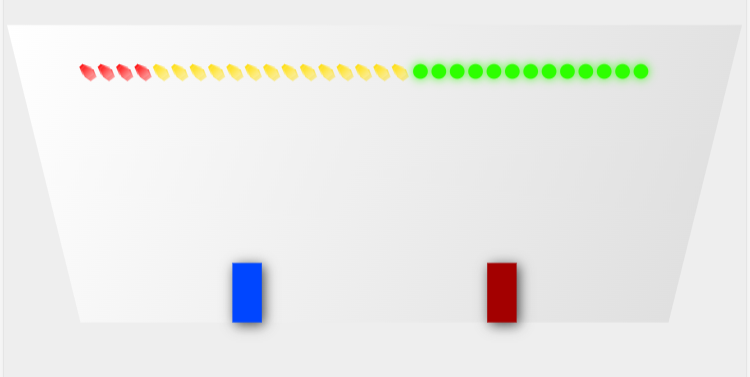
\includegraphics[width=0.9\linewidth]{led_vis.png}
    \caption{Voorbeeld LED visualisatie (2 fosforen, 1 QD en 2 LEDs)}%
    \label{fig:led_vis}
\end{figure}

\section{Implementatie hyperspectral image rendering}

Voor hyperspectral image rendering gebruiken we net zoals voor color rendering de luxpy bibliotheek ~\cite{smetTutorialLuxPyPython2020}. Als we echter gewoon de standaard implementatie gebruiken zorgt het in dit geval voor problemen. Dit omdat het uitvoeren van de standaardimplementatie op de server maar liefst 15 minuten duurt. Daarnaast gebruikt deze methode ook een grote hoeveelheid geheugen. Als dus
meerdere mensen tegelijk deze standaardimplementatie zouden gebruiken zou de server al rap niet genoeg geheugen hebben en crashen. Daarnaast vinden we 15 minuten zeker een stuk te lang voor een gebruiker om te wachten op het resultaat van de rendering. 

Om dit probleem op te lossen onderzochten we twee mogelijke oplossingen:
\begin{itemize}
    \item Aanpassen van de gebruikte foto.
    \item Berekeningen die niet veranderen opslaan.
\end{itemize} 

\subsection{Foto}

De standaard foto \ref{fig:std_img_luxpy} die luxpy ~\cite{smetTutorialLuxPyPython2020} gebruikt is een vrij complexe foto met een hoge
resolutie. Deze combinatie van de hoge resolutie en de vele kleueren in de foto
zorgt ervoor dat de berekeningen langer duren dan gewenst. Om dit op te lossen keken we naar twee oplossingen:

\begin{itemize}
    \item Resolutie verlagen
    \item Complexiteit foto verlagen
\end{itemize}

\begin{figure}[H]
    \centering
    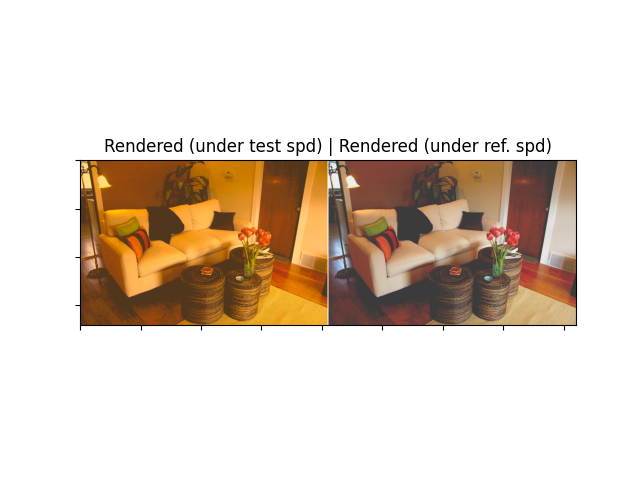
\includegraphics[width=0.8\linewidth]{standard_image.png}
    \caption{Standaard foto luxpy ~\cite{smetTutorialLuxPyPython2020}}%
    \label{fig:std_img_luxpy}
\end{figure}

Ten eerste onderzochten we het gebruik van een simpelere foto. We gebruikten hiervoor eerst een heel simpele foto van een blauwe bal \ref{fig:blue_ball} op een witte achtergrond. Dit verbeterde de snelheid van de berekening sterk, maar bracht een belangrijk probleem met zich mee: de foto geeft weinig informatie over de belichting.

Het grootste probleem is namelijk dat een gebruiker niet kan weten hoe de bal er normaal uitziet. Er bestaan namelijk zeer veel blauwe ballen in zeer veel verschillende tinten blauw. Het is dus hierdoor ook moeilijk af te leiden wat het effect van de gebruikte belichting is. De gebruiker kan dus niet leren over de effecten van de belichting op de kleur van het object.

\begin{figure}[H]
    \centering
    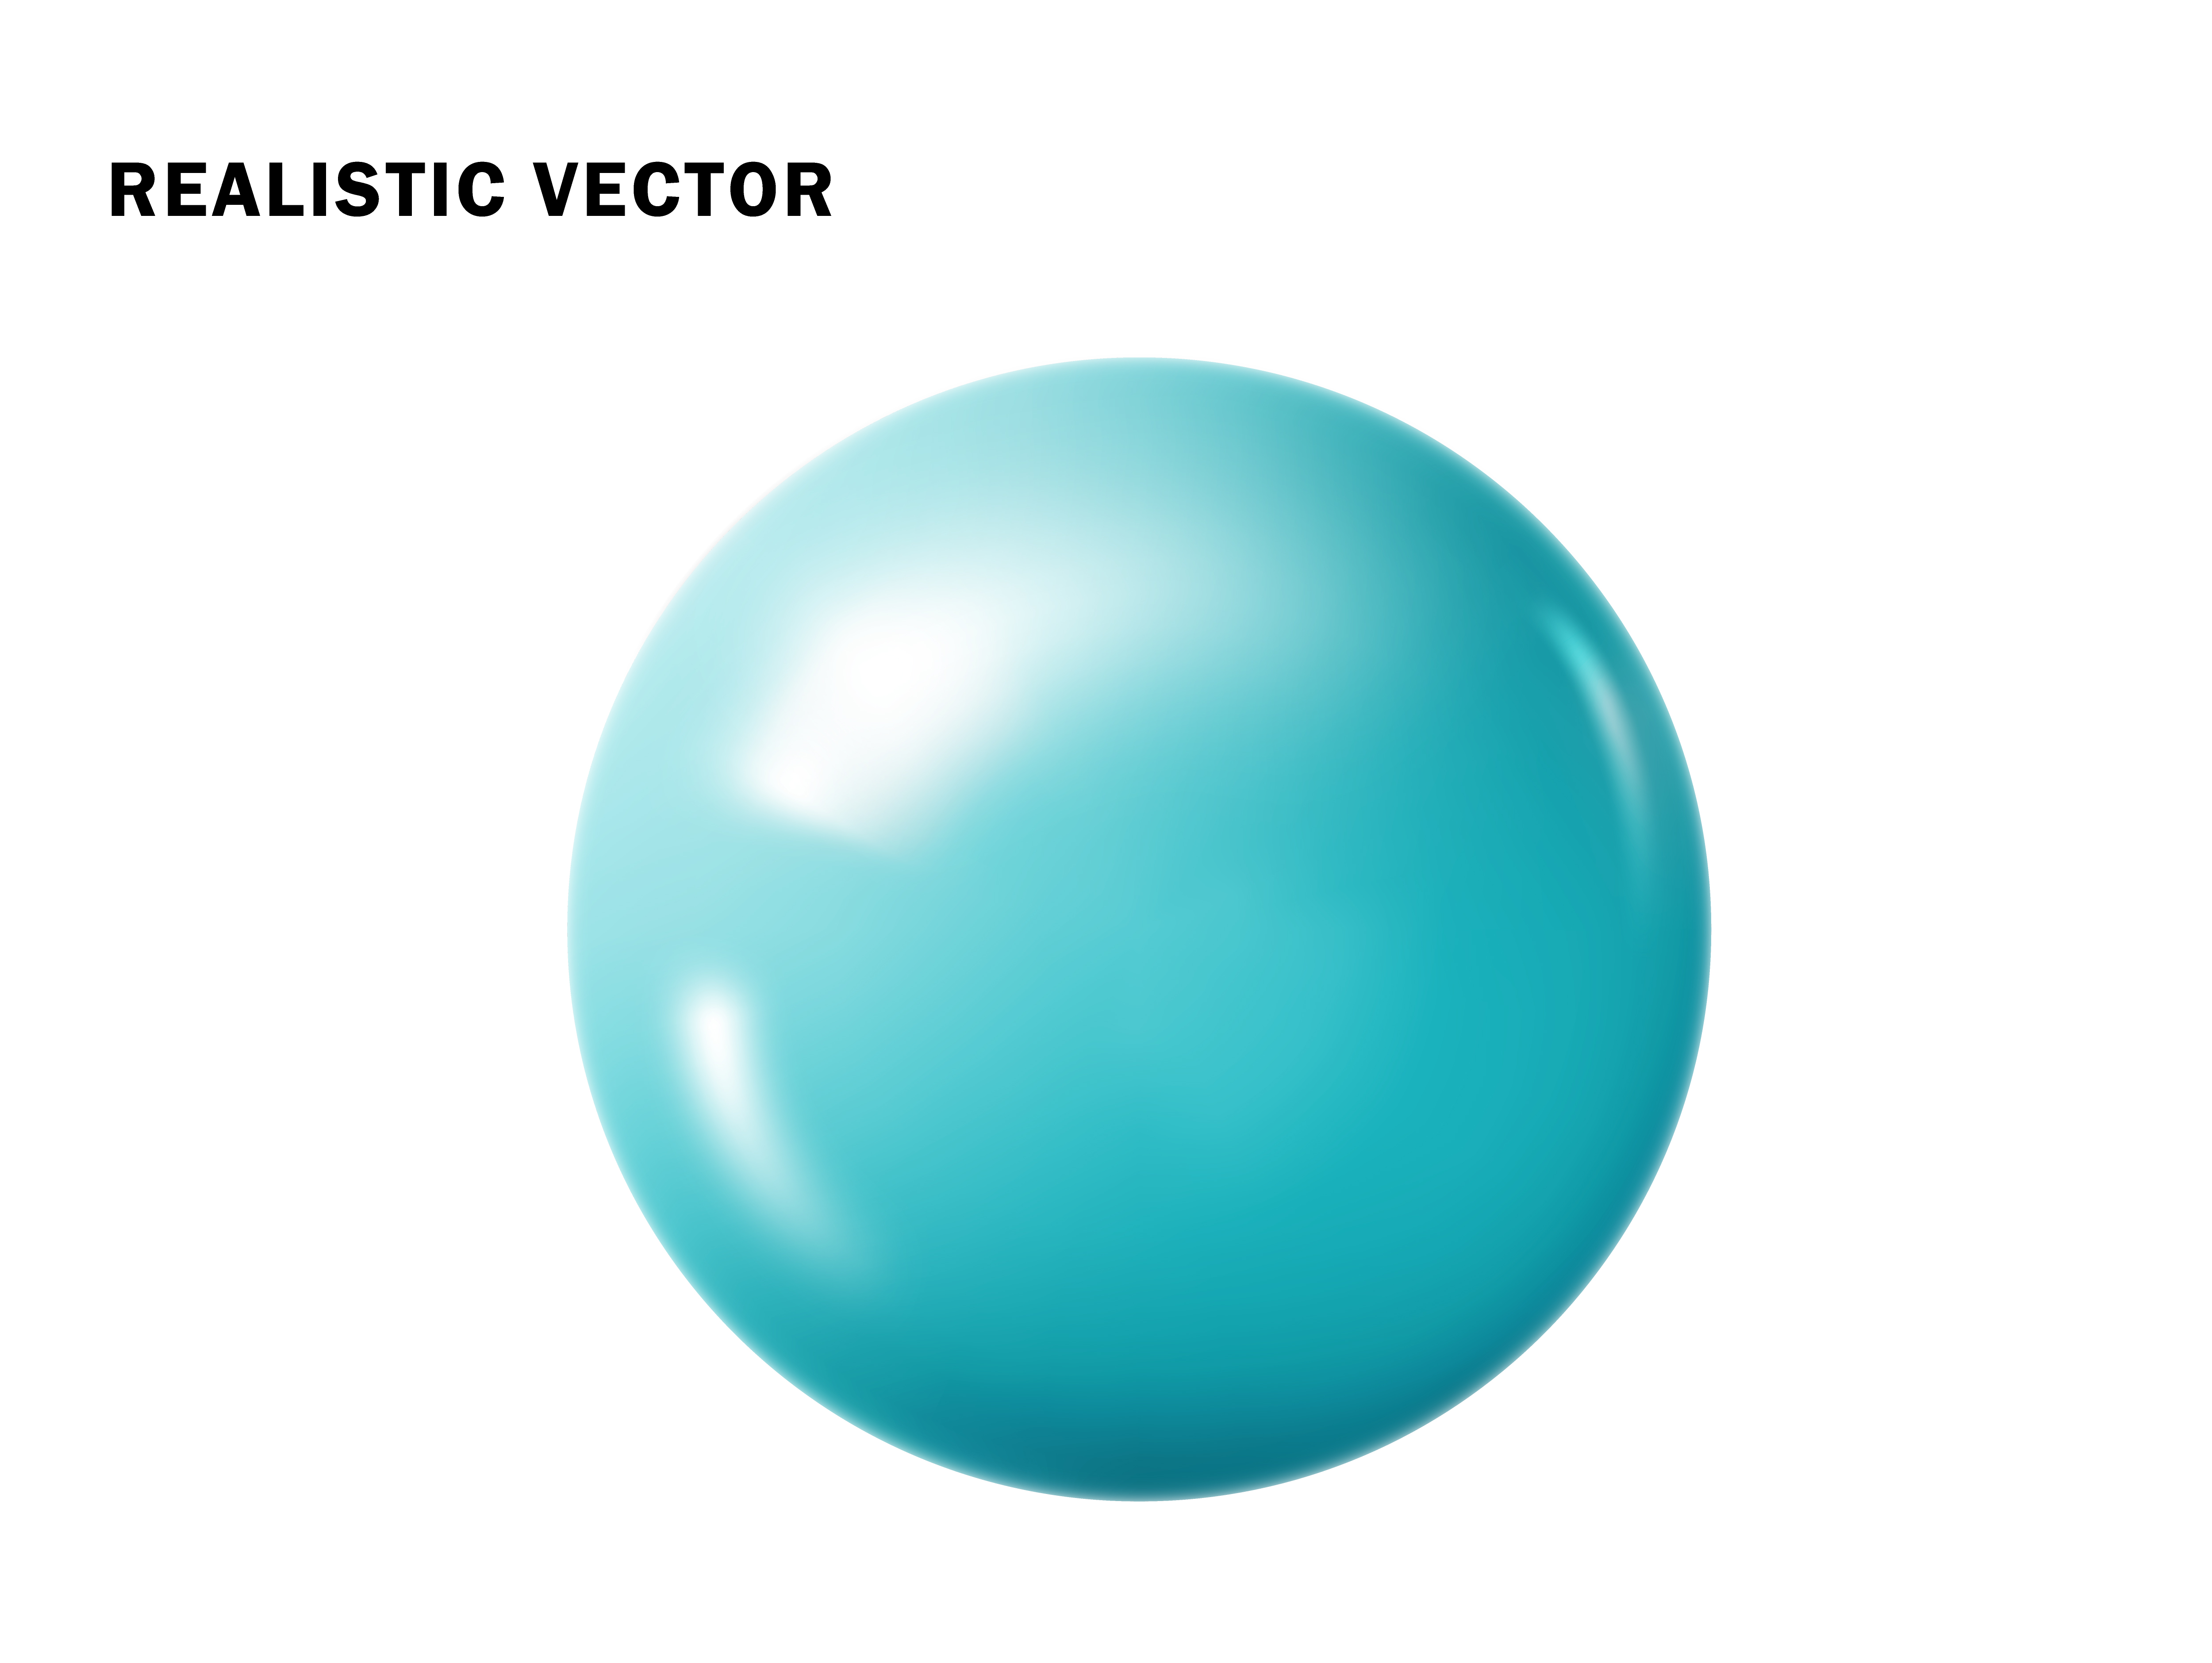
\includegraphics[width=0.4\linewidth]{blue_ball_copyright.jpg}
    \caption{Foto blauwe bal}%
    \label{fig:blue_ball}
\end{figure}

Om dit op te lossen keken we naar een eenvoudigere foto, die echter wel voorwerpen bevat waarvan de gebruiker de kleur zeker kent. Zo kwamen we op het idee om een verzameling fruit op een witte achtergrond te gebruiken, zoals te zien is in Figuur \ref{fig:fruit}.

Hierdoor blijft de hoeveelheid kleuren beperkt en hebben waardoor de versnelling optreed. Daarnaast hebben de meeste voorwerpen een vaste kleur wat ervoor zorgt dat de gebruiker de normale kleur van de voorwerpen kent. Deze verbetering zorgde echter nog niet voor genoeg winst in snelheid, dus onderzochten we ook de resolutie.

\begin{figure}[H]
    \centering
    \includegraphics[width=0.6\linewidth]{fruit_nocopyright.jpg}
    \caption{Foto fruit 6,99MB}%
    \label{fig:fruit}
\end{figure}

Ten tweede keken we naar de resolutie van de foto. Dit betekende simpelweg dat we de foto verkleinden. We deden dit systematisch totdat we een versie kregen die zowel een voldoende snelle berekening als een scherp genoeg beeld opleverde. Uiteindelijk verkleinden we de foto van 6,99 MB naar 9,09 kB, zoals te zien is in Figuur \ref{fig:fruit_small}. Het is mogelijk de foto nog verder te verkleinen, maar dit zou ten koste gaan van de kwaliteit van de foto. We vonden dat de kwaliteit van de foto in Figuur \ref{fig:fruit} nog voldoende was om de gebruiker een goed beeld te geven van de belichting van de foto. Bij kleinere foto's beginnen bepaalde details verloren te gaan, wat het moeilijker maakt voor de gebruiker om de belichting correct in te schatten.

\begin{figure}[H]
    \centering
    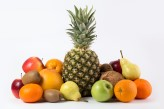
\includegraphics[width=0.6\linewidth]{fruit_nocopyright_3.jpg}
    \caption{Foto fruit 9,09kB}%
    \label{fig:fruit_small}
\end{figure}

Met een combinatie van deze twee aanpassingen op de foto bekomen we een foto die snel genoeg is ($\pm$ 5 seconden) om te renderen en toch voldoende informatie bevat voor de gebruiker.

\subsection{Berekeningen}

Om de berekening nog sneller te maken keken we ook naar het opslaan van niet veranderende berekeningen. Zo zal de rendering van de verschillende beschikbare referentiespectra bijvoorbeeld nooit veranderen. We kunnen de rendering van de referentiespectra dus opslaan en deze opnieuw gebruiken bij elke berekening van de rendering.

Deze aanpassing zorgt ervoor dat de rendering zelf een stuk sneller kan verlopen doordat, maar half zo veel werk moet gebeuren. Doordat we echter reeds de tijd van de berekening sterk verlaagt hebben door de aanpassingen aan de foto, is het effect van deze aanpassing minder groot. Doordat de resolutie voor een grote verandering in tijd zorgt, treed er een probleem op bij het voordien berekenen van de foto. Door de lage resolutie is namelijk de tijd die nodig is voor het berekenen van het referentiespectra gedeelte ongeveer gelijk aan de tijd die nodig is voor het inladen van de foto. Hierdoor is het effect van het voordien berekenen van het referentiespectra verwaarloosbaar. Moesten we echter in de toekomst een foto met een grotere resolutie willen gebruiken kan deze aanpassing mogelijks wel een voldoende groot effect hebben.

\section{Implementatie data manager}\label{sec:data_manager}

We maken de app bruikbaarder voor geavanceerde gebruikers door een data manager toe te voegen. Hierin krijgt de gebruiker de mogelijkheid om gebruikte defaults aan te passen en te bekijken. Daarnaast kan de gebruiker eigen luminescente materialen toevoegen.

De eerste functie in de data manager is het vergrendelen van bepaalde variabelen. Met deze functionaliteit kan de gebruiker verschillende parameters van de inputs vergrendelen of ontgrendelen. Dit is vooral bedoeld voor educatieve doeleinden, bijvoorbeeld wanneer een docent leerlingen vraagt om een specifieke waarde, zoals de excitatiebreedte, vast in te stellen.

Daarnaast kan de gebruiker het referentiespectrum voor de realistic rendering aanpassen. Hierbij kan hij kiezen uit standaard spectra zoals D65, Tungsten, Clear Sky en Daylight. Voor color rendering kan hij bovendien het CRI-type instellen (CIE Ra-15, IES TM-30).

Ten derde kan de gebruiker de formules voor de standaard spectra van luminescente materialen en het LED-emissiemodel aanpassen. Hij kan gebruikmaken van standaard formules en parameters om een wiskundige formule te defini\"eren voor de spectra van de luminescente materialen. Deze formule kan vervolgens worden in- of uitgeschakeld. Tijdens het maken van de formule tonen we een grafiek van het gegenereerde spectrum om het beslissingsproces te vergemakkelijken.

\begin{figure}[H]
    \centering
    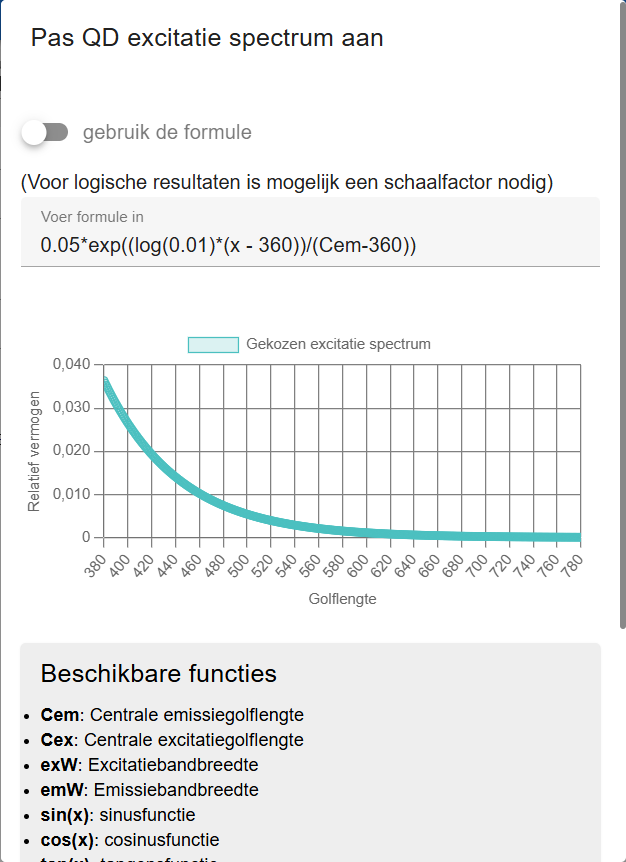
\includegraphics[width=0.5\linewidth]{Formula_input.png}
    \caption{Voorbeeld input formule}%
    \label{fig:formula_input}
\end{figure}

Ten vierde krijgt de gebruiker in de data manager inzicht in de verschillende gebruikte standaardparameters. Zo kan hij de standaard EQE-waarden, het standaard LED-emissiemodel en de eigenschappen van luminescente materialen bekijken. Daarnaast tonen we bij de EQE- en LED-emissiemodeldata ook de bron van deze gegevens.

Zoals eerder vermeld, kan de gebruiker ook eigen luminescente materialen toevoegen \ref{sec:luminescent_input}. Tot slot kan hij de gebruikte \gls{eqe}-waarden aanpassen. Dit gebeurt via een \gls{csv}-bestand, zoals beschreven in \ref{sec:eqe}.

\section{Hosting}

De webapp wordt gehost op een combinatie van nginx (frontend) en systemctl (Flask-backend). Nginx fungeert niet alleen als host voor de frontend, maar ook als reverse proxy. Hierdoor kan het de requests van de frontend naar de backend sturen en tegelijkertijd rate limiting toepassen. Dit voorkomt overbelasting van de server, vooral bij rekenintensieve processen zoals hyperspectral image rendering, die veel tijd in beslag nemen.
% \chapter{Feedback van gebruikers}\label{ch:user-feedback}

misschien niet
\chapter{Uitbreidingen}\label{ch:uitbreidingen}

De webapp bevat alle belangrijkste functionaliteiten. We zouden nog enkele concepten, zoals de ''melanopic eye sensitivity'', kunnen toevoegen. Dit concept meet hoe gevoelig het menselijk oog is voor licht. Toch hebben we besloten om dit en andere complexe concepten niet op te nemen, omdat ze de webapp onnodig ingewikkeld zouden maken. Ons doel is om de webapp zo eenvoudig en toegankelijk mogelijk te houden.

Naast het toevoegen van concepten kunnen we de webapp ook uitbreiden met extra functionaliteiten. Zo kunnen we bijvoorbeeld gebruikers de mogelijkheid geven om een account aan te maken. Met dit account kunnen zij instellingen, \gls{led}-configuraties en andere persoonlijke voorkeuren permanent opslaan.

Daarnaast kunnen we het educatieve aspect van de webapp verder uitbreiden. Momenteel ligt de focus vooral op interactiviteit en experimentatie. We kunnen echter extra educatieve elementen toevoegen, zoals uitleg over de gebruikte concepten en oefeningen om de leerervaring te verdiepen.

\section{Gamification}

Zoals eerder vermeld, kan de webapp uitgebreid worden met meer educatieve aspecten. Gamification is een populaire methode om dit te realiseren ~\cite{saleemGamificationApplicationsElearning2022}. Dit houdt in dat we game-elementen toevoegen aan een educatieve app, zonder dat het een volledige game wordt. In tegenstelling tot ''Game-based learning'', waarbij leren plaatsvindt door een spel te spelen, verhoogt gamification de motivatie en aandacht van de gebruiker door spelelementen te integreren. Hierdoor leert de gebruiker meer en beter.

Veelgebruikte game-elementen zijn:
\begin{itemize}
  \item punten
  \item uitdagingen
  \item levels
  \item klassementen
  \item badges
\end{itemize}

Deze elementen houden niet alleen de gebruiker gemotiveerd, maar stimuleren ook interactie en discussie tussen gebruikers of studenten. Dit bevordert wederzijds leren en kan leiden tot een gezonde competitie binnen de gebruikersgroep.

\section{Analyse model luminescente materialen}

Het geavanceerde model (\cref{sec:advanced}) voor de luminescente materialen is momenteel ge\"implementeerd in de app, maar nog niet vergeleken met experimentele data. De app gebruikt dit model uitsluitend op basis van het beschikbare bewijs. Daarom is het belangrijk om het model te toetsen aan experimentele data. Dit bevestigt de correctheid en biedt de mogelijkheid om het model verder te optimaliseren.

Voor de excitatie- en emissiespectra gebruiken we eenvoudige formules, maar deze kunnen we uitbreiden met geavanceerdere formules die beter aansluiten op de realiteit. Daarnaast kunnen we meerdere standaardformules aanbieden, zodat zowel algemene als specifieke formules beschikbaar zijn. De gebruiker kiest vervolgens zelf welke formule hij of zij wil gebruiken.





\chapter{Conclusie}\label{ch:conclusie}

% % !TeX root = thesis.tex


%Het eerste hoofdstuk van je thesis.
\chapter{Changes w.r.t. the default template}\label{ch:introduction}



\begin{itemize}
\item Changed font from default computer modern to CMBright.
\item Verhoogde baseline-skip in de titel. Zodat letters niet tegen elkaar plakken
\item Siunitx package auto toegevoegd zie gebruik: \url{https://github.com/dramco-edu/LaTex/wiki/LaTex-Tips-and-Tricks#using-si-units-numbers-angles-etc}
\item Gebruik nu formules inclusief eenheden via het commando:
\begin{lstlisting}
    \begin{equation}
     E = m c^2
     \tagaddtext{[\si{\joule}]}
    \end{equation}
    \end{lstlisting},
which outputs:
\begin{equation}\label{eq:emc2}
    E = m c^2%
    \tagaddtext{[\si{\joule}]}
\end{equation}
\item Afkortingen:
\begin{itemize}
    \item  \gls{iot}      % outputs (if first occurance): Internet-of-Things (IoT)
          % outputs (else): IoT
    \item \glspl{lpwan}  % outputs (if first occurance): Low-Power Wide-Area Networks (LPWANs)
          % outputs (else): LPWANs
    \item \acrlong{iot}  % outputs: Internet-of-Things
    \item \acrshort{iot} % outputs: IoT
    \item \acrfull{iot}  % outputs: Internet-of-Things (IoT)
\end{itemize}
\item \verb!\ce{CO2}! \ce{CO2}
\item Refs:
\begin{itemize}

    \item \cref{fig:example}
    \item \cref{tab:example}
    \item \cref{ch:introduction}
    \item \cref{eq:emc2}


    \item \verb!\cref{fig:example}! becomes \cref{fig:example}
    \item \verb!\cref{tab:example}! becomes \cref{tab:example}
    \item \verb!\cref{ch:introduction}! becomes \cref{ch:introduction}
    \item \cref{eq:emc2}


\end{itemize}
\item numerical citation~\cite{s19030585}
\begin{itemize}
    \item \verb!\cite{callebaut10lorawan}! becomes \cite{callebaut10lorawan}

    \item \verb!\citeauthor{callebaut10lorawan}! becomes \citeauthor{callebaut10lorawan}
    \item \verb!\citeauthorref{callebaut10lorawan}! becomes \citeauthorref{callebaut10lorawan}
    \item \verb!\autocite[chap.~2]{callebaut10lorawan}! becomes \autocite[chap.~2]{callebaut10lorawan}
    \item \verb!\footcite{callebaut10lorawan}! becomes \footcite{callebaut10lorawan}
    \item \verb!\fullcite{callebaut10lorawan}! becomes \fullcite{callebaut10lorawan}
\end{itemize}

    \item A $\SI{45}{\degree}$ angle or a \ang{45}.

    \item It is \SI{17}{\degreeCelsius} outside.

    \item  \num{10000}
    \item \num{3.45d-4}

    \item \si{\kilo\gram\meter\per\square\second} 
    \item \si{kg.m/s^2} %unit only

    \item \SI{10}{\percent}
    \item \SI{68}{kg}
\end{itemize}


\begin{center}
    \begin{tabular}{ l  l  l  p{5cm}}
        \hline
        Day       & Min Temp & Max Temp & Summary                                                      \\ \hline
        Monday    & 11C      & 22C      & A clear day with lots of sunshine.
        However, the strong breeze will bring down the temperatures.                                   \\ \hline
        Tuesday   & 9C       & 19C      & Cloudy with rain, across many northern regions. Clear spells
        across most of Scotland and Northern Ireland,
        but rain reaching the far northwest.                                                           \\ \hline
        Wednesday & 10C      & 21C      & Rain will still linger for the morning.
        Conditions will improve by early afternoon and continue
        throughout the evening.                                                                        \\
        \hline
    \end{tabular}
\end{center}







\newcolumntype{R}{>{\raggedleft\arraybackslash}X}%


\begin{center}
    \begin{tabularx}{\textwidth}{ cccX }
        \hline
        Day       & Min Temp & Max Temp & Summary                                                      \\ \hline
        Monday    & 11C      & 22C      & A clear day with lots of sunshine.
        However, the strong breeze will bring down the temperatures.                                   \\ \hline
        Tuesday   & 9C       & 19C      & Cloudy with rain, across many northern regions. Clear spells
        across most of Scotland and Northern Ireland,
        but rain reaching the far northwest.                                                           \\ \hline
        Wednesday & 10C      & 21C      & Rain will still linger for the morning.
        Conditions will improve by early afternoon and continue
        throughout the evening.                                                                        \\
        \hline
    \end{tabularx}
\end{center}



\begin{figure}
    \centering
    
\includegraphics[width=0.95\linewidth]{example.jpg}
    \caption{Example JPG}%
    \label{fig:example}
\end{figure}

\begin{table}[ht]
    \centering
    \caption{Fixed-width columns.}%
    \label{tab:example}
    \begin{tabular}[t]{l>{\raggedright}p{0.3\linewidth}>{\raggedright\arraybackslash}p{0.3\linewidth}}
        \toprule
                     & Treatment A                    & Treatment B                     \\
        \midrule
        John Smith   & Good response, no side-effects & No response                     \\
        Jane Doe     & --                             & Good response, no side-effects  \\
        Mary Johnson & No response                    & Good response with side-effects \\
        \bottomrule
    \end{tabular}
\end{table}%



\begin{listing}[ht]
    \inputminted{python}{code/example.py}
    \caption{Minimal working example}
    \label{listing:1}
\end{listing}

\begin{figure}
    \centering
    % This file was created by tikzplotlib v0.9.8.
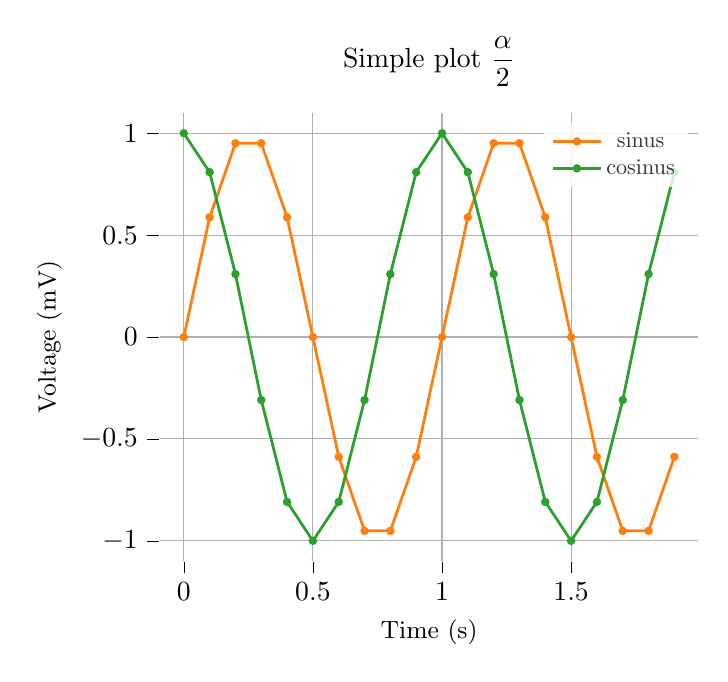
\begin{tikzpicture}



\begin{axis}[
axis line style={white},
tick align=outside,
tick pos=left,
title={Simple plot \(\dfrac{\alpha}{2}\)},
xlabel={Time (\si{\second})},
xmajorgrids,
xmin=-0.095, xmax=1.995,
ylabel={Voltage (\si{\milli\volt})},
ymajorgrids,
ymin=-1.1, ymax=1.1,
]
\addplot [color0, mark=*]
table {%
0 0
0.1 0.587785252292473
0.2 0.951056516295154
0.3 0.951056516295154
0.4 0.587785252292473
0.5 1.22464679914735e-16
0.6 -0.587785252292473
0.7 -0.951056516295154
0.8 -0.951056516295154
0.9 -0.587785252292473
1 -2.44929359829471e-16
1.1 0.587785252292474
1.2 0.951056516295154
1.3 0.951056516295154
1.4 0.587785252292473
1.5 3.67394039744206e-16
1.6 -0.587785252292473
1.7 -0.951056516295154
1.8 -0.951056516295154
1.9 -0.587785252292473
};
\addlegendentry{sinus}
\addplot [color1, mark=*]
table {%
0 1
0.1 0.809016994374947
0.2 0.309016994374947
0.3 -0.309016994374948
0.4 -0.809016994374947
0.5 -1
0.6 -0.809016994374947
0.7 -0.309016994374948
0.8 0.309016994374947
0.9 0.809016994374947
1 1
1.1 0.809016994374947
1.2 0.309016994374947
1.3 -0.309016994374947
1.4 -0.809016994374947
1.5 -1
1.6 -0.809016994374948
1.7 -0.309016994374946
1.8 0.309016994374947
1.9 0.809016994374947
};
\addlegendentry{cosinus}
\end{axis}

\end{tikzpicture}

    \caption{Caption}
    \label{fig:my_label}
\end{figure}

% % !TeX root = thesis.tex

%second chapter of your thesis
\chapter{Bespreking}
In het vorig hoofdstuk hebben we naar deze tekst verwezen\label{verwijzing}.

%% !TeX root = thesis.tex

%%%%%%%%%%%%%%%%%%%%%%%%%%%%%%%%%%%%%%%%%%%%%%%%%%%%%%%%%%%%%%%%%%% 
%                                                                 %
%                            CHAPTER                              %
%                                                                 %
%%%%%%%%%%%%%%%%%%%%%%%%%%%%%%%%%%%%%%%%%%%%%%%%%%%%%%%%%%%%%%%%%%% 
 
\chapter{This is the another Chapter}
 
You can say great work has been done about something \citep{Castleman98,Granlund95} or say that \citet{Holmes95} did something really great.
xxxx xxxxx xxxx xxxxxxxxx 
xxx xxxxx xxxxx xxx xxxx xxxx xxxxx xxxxx xxxx xxxxx xxxx xxxxxxxxx
 
\begin{figure}
\vspace{2.0in}
\caption{This is the Caption for Figure 1}
\end{figure}
 
xxx xxxxx xxxxx xxx xxxx xxxx xxxxx xxxxx xxxx xxxxx xxxx xxxxxxxxx
xxx xxxxx xxxxx xxx xxxx xxxx xxxxx xxxxx xxxx xxxxx xxxx xxxxxxxxx
xxx xxxxx xxxxx xxx xxxx xxxx xxxxx xxxxx xxxx xxxxx xxxx xxxxxxxxx
 
\begin{table}[t]
\begin{center}
\begin{tabular}{lll}
Here's       & an          & example  \\
of           & a           & table    \\
floated      & with        & the      \\
\verb+table+ & environment & command.
\end{tabular}
\end{center}
\caption{This is the Caption for Table 1}
\end{table}
 
xxx xxxxx xxxxx xxx xxxx xxxx xxxxx xxxxx xxxx xxxxx xxxx xxxxxxxxx
xxx xxxxx xxxxx xxx xxxx xxxx xxxxx xxxxx xxxx xxxxx xxxx xxxxxxxxx
 
\section{This is a Section Heading}
 

% This will ensure ALL entries in bib.bib appear in the bibliography
% \nocite{*}

% Bibliografie: referenties. De items zitten in bib.bib
%%%%%%%%%%%%%%%%%%%%%%%%%%%%%%%%%%%%%%%%%%%%%%%%%%%%%%%%%%%%%%%%%
\printbibliography

% Eventueel enkele appendices
%%%%%%%%%%%%%%%%%%%%%%%%%%%%%%
\appendix
\chapter{Een aanhangsel}
sdfsffqsfsf

% Bijlage met daarin het wetenschappelijk artikel
%%%%%%%%%%%%%%%%%%%%%%%%%%%%%%%%%%%%%%%%%%%%%%%%%%
\chapter{Beschrijving van deze masterproef in de vorm van een wetenschappelijk artikel}
The thesis should also contain a short scientific article. If you write your thesis in Dutch, you must write the article in English, and vice versa. We advise you to employ the IEEE Manuscript Templates for Conference Proceedings (\url{https://www.overleaf.com/latex/templates/ieee-conference-template/grfzhhncsfqn}).
Compile the article in another project and include the generated pdf file as shown below:

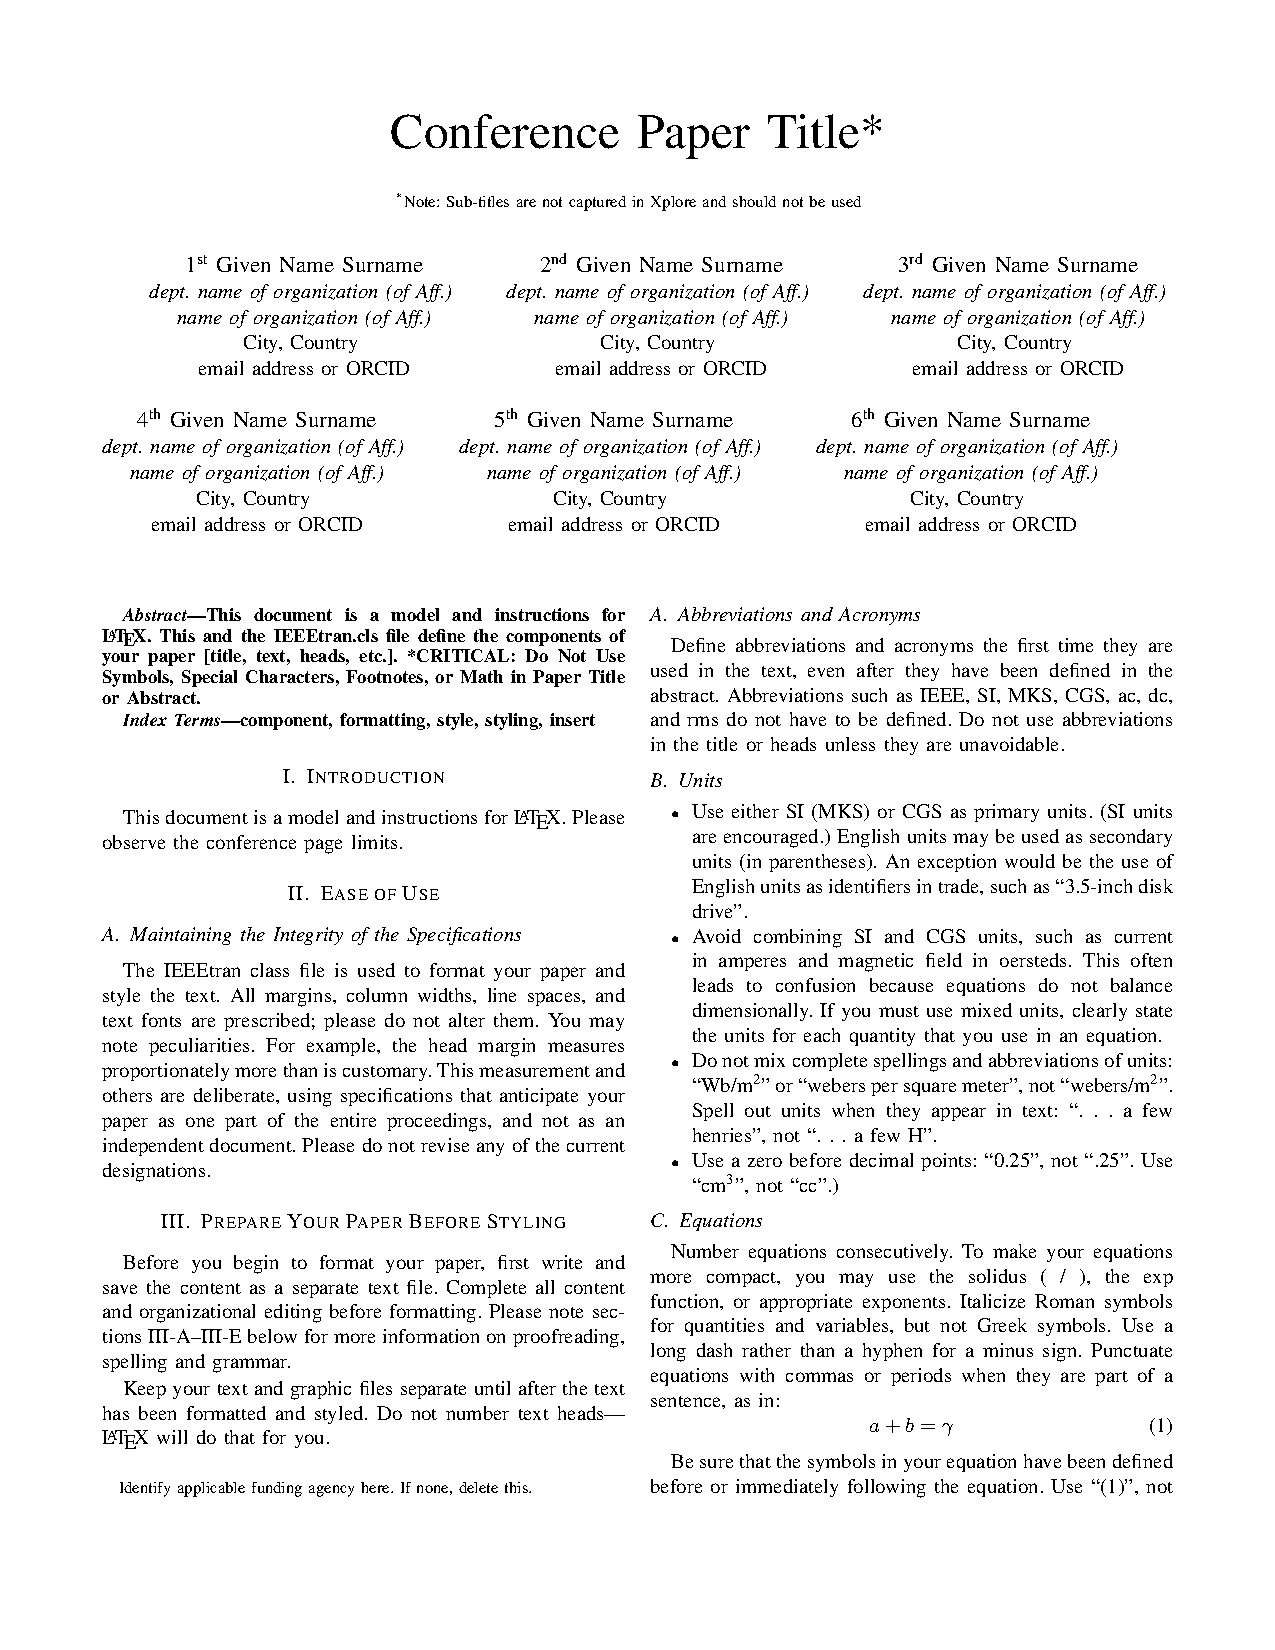
\includepdf{article.pdf}

% Bijlage met daarin de poster
%%%%%%%%%%%%%%%%%%%%%%%%%%%%%%%
\chapter{Poster}
%\includepdf{poster.pdf}

\chapter{GenAI code of conduct for students}

Generative AI (GenAI) assistance tools can be used to generate text, image, code, video, music, or combinations of these. It includes typical tools like (but this list is not limited to): ChatGPT, Google Gemini, MS Copilot, Midjourney, Claude.ai, Perplexity.ai, Dall-E, etc.

\section*{Student Information}
\begin{tabbing}
\makeatletter% required keep
Student name: \@forenameA \ \@surnameA
\makeatother
\end{tabbing}

This form is related to my Master thesis. \\
\makeatletter% required keep
Title Master thesis: \@title \hspace{1cm} Promoter: \underline{\hspace{5cm}}\\
Daily supervisor: \underline{\hspace{5cm}}
\makeatother


\section*{Use of GenAI Assistance}
Please indicate with "X" (possibly multiple times) in which way you were using GenAI:

\begin{itemize}
    \item[$\Box$] I did not use any GenAI assistance tool.
    \item[$\Box$] I did use GenAI assistance. In this case, specify which ones (e.g., ChatGPT, \ldots): \underline{\hspace{5cm}}
\end{itemize}

\section*{GenAI Assistance Used As/For}
\begin{itemize}
    \item[$\Box$] MS Copilot \\
    \item[$\Box$] Language assistance \\
    \item[$\Box$] Search engine \\
    \item[$\Box$] Literature search \\
    \item[$\Box$] Short-form input assistance \\
    \item[$\Box$] Generating programming code \\
    \item[$\Box$] Generating new research ideas \\
    \item[$\Box$] Generating blocks of text \\
    \item[$\Box$] Other (specify): \underline{\hspace{5cm}}
\end{itemize}

\section*{Code of Conduct for Different Uses}
\subsection*{Language Assistant for Reviewing or Improving Texts}
This use is similar to using spelling and grammar check tools, and you do not have to refer to the use of GenAI in the text. Be careful:
\begin{itemize}
    \item Using GenAI tools on texts you did not write yourself to cover up plagiarism (by paraphrasing original texts) is not allowed.
\end{itemize}

\subsection*{Search Engine for Information or Existing Research}
This use is similar to a Google search or checking Wikipedia. If you then write your own text based on this information, you do not have to refer to the use of GenAI in the text. Be careful:
\begin{itemize}
    \item Be aware that the output of the GenAI tool cannot be guaranteed as a 100\% reliable source of information.
    \item The output may not be entirely correct and is limited due to the databases it uses. Knowledge evolves and may change over time, and it may be that the database of the GenAI tool is not up to date.
\end{itemize}

\subsection*{Literature Search}
This use is comparable to a Google Scholar search. Be careful:
\begin{itemize}
    \item Be aware that the output is restricted to the database it is built on. After this initial search, look for scientific sources and conduct your own analysis.
    \item GenAI tools (like ChatGPT) may output no or wrong references. As a student, you are responsible for further checking and verifying the accuracy of references.
\end{itemize}

\subsection*{Short-form Input Assistance}
This use is similar to Google Docs powered by generative language models.

\subsection*{Generating Programming Code}
The use of GenAI for coding should be explicitly allowed by the teacher. If used for coding, correctly mention the use of GenAI assistance and cite it.

\subsection*{Generating New Research Ideas}
Further verify whether the idea is novel or not. It is likely that it is related to existing work, which should be referenced.

\subsection*{Generating Blocks of Text}
Inserting blocks of text without quotes and a reference to GenAI assistance in your report or thesis is not allowed. Be careful:
\begin{itemize}
    \item When you literally copy elements from a conversation with a GenAI tool, quote them between quotation marks and refer to them according to the specified reference style.
    \item Describe the use of the GenAI tool (tool name, version, date, etc.) in the method section and optionally add the full conversation as an attachment.
\end{itemize}

\subsection*{Other}
Contact the professor of the course or the promoter of the thesis. Inform also the program director. Motivate how you comply with Article 84 of the exam regulations. Explain the use and added value of ChatGPT or another AI tool.

\section*{Further Important Guidelines and Remarks}
\begin{itemize}
    \item GenAI assistance cannot be used related to data or subjects under Non-Disclosure Agreement.
    \item GenAI assistance cannot be used related to sensitive or personal data due to privacy issues.
    \item Take a scientific and critical attitude when interacting with GenAI assistance and interpreting its output.
    \item As a student, you are responsible for complying with Article 84 of the exam regulations: your report or thesis should reflect your own knowledge, understanding, and skills.
\end{itemize}

\subsection*{Exam Regulations Article 84}
``Every conduct individual students display with which they (partially) inhibit or attempt to inhibit a correct judgement of their own knowledge, understanding and/or skills or those of other students, is considered an irregularity which may result in a suitable penalty. A special type of irregularity is plagiarism, i.e., copying the work (ideas, texts, structures, designs, images, plans, codes, \ldots) of others or prior personal work in an exact or slightly modified way without adequately acknowledging the sources.''

\subsection*{Additional Reading}
More information about being transparent on the use of GenAI assistance and about citing and referencing GenAI can be found on the student website.

\subsection*{A Few Final Words}
If you are uncertain whether or not you should declare your use of AI tools, discuss the matter with your teacher or promoter. It is safer to declare AI use when it is not needed than to withhold that declaration when it is required.

Finally, remember that advanced AI tools are new and that they can do things they could not do until recently. It is important to follow up on the most recent developments in AI technologies and communicate openly with your teachers, assistants, supervisors, and peers.



\end{document}
